\chapter{操作系统与程序运行环境}\label{os-ch1}

程序执行一条普通加法指令时，通常直接使用处理器；读取文件时，却不能自己任意驱动磁盘。两种操作的差别来自资源保护：处理器、内存和设备由多个程序共享，操作系统必须管理它们，并给应用提供受控的使用接口。本章先沿一次程序运行建立用户态、内核态、异常、系统调用和地址空间之间的关系。

\section{操作系统管理什么，向程序提供什么}\label{os-1-1}

\textbf{操作系统}是控制和管理计算机硬件、软件资源，组织程序运行，并向用户和应用程序提供接口的系统软件。这里的``管理''要落到具体对象上：处理机管理决定谁运行；内存管理分配空间并隔离访问；文件管理组织持久数据；设备管理协调输入输出，屏蔽设备差异。

面向用户的命令行、图形界面便于发起操作；面向应用程序的系统调用接口允许程序请求内核服务。图形界面不是所有操作系统都必须具有的组成部分。编译器虽然也是系统软件，但把高级语言翻译成目标程序不因此成为操作系统的基本职责。

\noindent{}〖1.1-003〗 下列哪项不是操作系统关心的基本问题：管理裸机、提供用户程序与硬件的接口、管理系统资源、提供高级语言编译器？答案是最后一项。判断依据是该功能是否承担资源管理与运行控制，不能只看它是否属于``系统软件''。

\subsection{并发、共享、虚拟与异步怎样联系}\label{os-c01-h13}

\textbf{并发}指多个活动在同一时间间隔内推进；\textbf{并行}指多个活动在同一时刻执行。一个 CPU 交替执行两个进程，已有并发；多个核上分别执行，才有处理器层面的并行。单 CPU 的计算与设备的数据传输仍可能并行。

\textbf{共享}指资源供多个并发活动共同使用。打印机一类资源通常需要互斥使用；磁盘文件或内存中只读代码可按规定共享。所谓``同时共享''不等于所有硬件操作都在同一瞬间发生，而是允许多个活动在同一时期使用同一资源。

\textbf{虚拟}把有限物理资源表现为若干逻辑资源。例如时间片让每个用户似乎独占一个处理器，虚拟内存让进程使用独立的地址空间。\textbf{异步}指进程因竞争处理器、等待 I/O 等原因，以不可预先确定的速度向前推进。它不表示进程内部可以违背程序依赖，也不等同于接口中的``异步 I/O''。

并发活动会竞争资源，因而需要共享与保护；虚拟化为并发活动提供合适的使用视图；资源等待又造成执行速度的不确定。后续同步与调度问题都以这些关系为前提。

\subsection{例 1-1　进程越多，处理器利用率一定越高吗}\label{os-ex1-1}

\noindent{}【2022】 下列关于多道程序系统的叙述中，不正确的是（　）。

A. 支持进程的并发执行　　B. 不必支持虚拟存储管理

C. 需要实现对共享资源的管理　　D. 进程数越多 CPU 利用率越高

\Needspace{6\baselineskip}

\textbf{解析。} 多道程序设计的直接收益是：一个进程等待 I/O 时，CPU 可以运行其他就绪进程。但这一收益有条件。可运行进程过多会增加调度开销和内存压力，严重时频繁换页，CPU 反而不能有效执行用户计算。因此 D 把条件性收益写成了单调关系，答案为 \textbf{D}。多道程序可以使用不带请求分页的内存方案，B 正确；``多道''不等于``必须有虚拟内存''。

\section{批处理、分时与实时解决不同的问题}\label{os-1-2}

早期人工装入程序时，CPU 常等待操作者准备下一项作业。单道批处理把多个作业预先排好，自动逐个执行，减少人工干预；但一个作业等待 I/O 时，处理器仍可能空闲。多道批处理允许多项作业同时在内存中，利用 CPU 与 I/O 的重叠提高吞吐量。中断使设备完成时能够通知 CPU，存储保护、调度和资源管理使多道运行可控。

\textbf{分时系统}把处理器时间分成时间片，轮流服务交互用户，主要关注响应时间和交互性。时间片不是每个程序的整个运行时间；未完成者会在以后继续执行。\textbf{实时系统}关注任务能否在规定期限内得到响应或完成。硬实时任务错过截止时间便不能满足系统要求；软实时允许一定程度的超期，但质量会下降。实时性不能只解释成``运行得快''：提前 1 秒与晚于期限 1 毫秒的结果，可能与绝对执行速度无关。

\begin{longtable}[]{@{}
  >{\raggedright\arraybackslash}p{(\columnwidth - 4\tabcolsep) * \real{0.2586}}
  >{\raggedright\arraybackslash}p{(\columnwidth - 4\tabcolsep) * \real{0.3697}}
  >{\raggedright\arraybackslash}p{(\columnwidth - 4\tabcolsep) * \real{0.3715}}@{}}
\toprule\noalign{}
\begin{minipage}[b]{\linewidth}\raggedright
类型
\end{minipage} & \begin{minipage}[b]{\linewidth}\raggedright
主要组织方式
\end{minipage} & \begin{minipage}[b]{\linewidth}\raggedright
评估时首先关心什么
\end{minipage} \\
\midrule\noalign{}
\endhead
\bottomrule\noalign{}
\endlastfoot
多道批处理 & 作业成批提交，运行中较少交互 & 吞吐量、周转时间、资源利用率 \\
分时 & 多用户交互，时间片轮转 & 响应时间、使用公平性 \\
实时 & 按期限和任务紧迫性组织执行 & 截止时间、响应的可预测性 \\
\end{longtable}

网络操作系统支持联网计算机上的资源与通信服务；分布式系统进一步组织多台计算机协作，可能提供统一资源视图。单用户、多用户、单任务、多任务则是另外的分类维度，不能把``单用户''自动理解为``单任务''。

\section{用户态、内核态与特权指令}\label{os-1-3}

处理器的\textbf{工作模式}规定当前代码能够执行哪些受保护操作。用二态模型表示时，用户态权限较低，内核态权限较高。模式位保存在程序状态信息中，由硬件按规则改变；普通用户程序不能通过一条普通赋值语句把自己变成内核态。

\textbf{特权指令}只能在规定的高权限模式执行，例如修改关键内存映射、设置中断屏蔽状态、直接控制受保护 I/O。若允许任意用户程序关闭时钟中断，它就可能长期占用 CPU，使调度失去控制。普通算术、逻辑和多数寄存器操作没有这种系统级影响，可以在用户态执行，也可以在内核态执行。

由此区分``必须在内核态运行''与``只有特权指令才能在内核态运行''。前者约束特权指令，后者把内核态误解成只能执行特权指令，无法完成内核中的普通计算。陷入指令是用户程序主动进入受控入口的指令；它允许在用户态执行，执行后由硬件转入规定的内核入口，不能据``会进入内核''反推它是用户态禁止执行的特权指令。

\section{中断和异常怎样把控制权交给内核}\label{os-1-4}

\textbf{外部中断}由正在执行的指令以外的事件引起，如时钟到期、设备完成。\textbf{异常}由当前指令执行过程中的事件引起，如除数为零、缺页、执行非法指令；主动执行陷入指令也通过受控异常入口请求服务。不同教材可能把``中断''作为包括内外事件的总称，本书需要区分时使用``外部中断''和``异常''。

一次典型控制转移包括以下连续过程：硬件检测事件，保存继续执行所需的断点和程序状态，按事件号找到处理入口并切换到所需模式；入口代码再保存会被处理程序改写的通用寄存器，执行处理；退出时恢复相应现场，使用专门返回指令恢复程序状态和继续位置。具体保存位置和硬件、软件分工取决于体系结构，不能把所有现场都归给同一方。

\begin{figure}
\centering
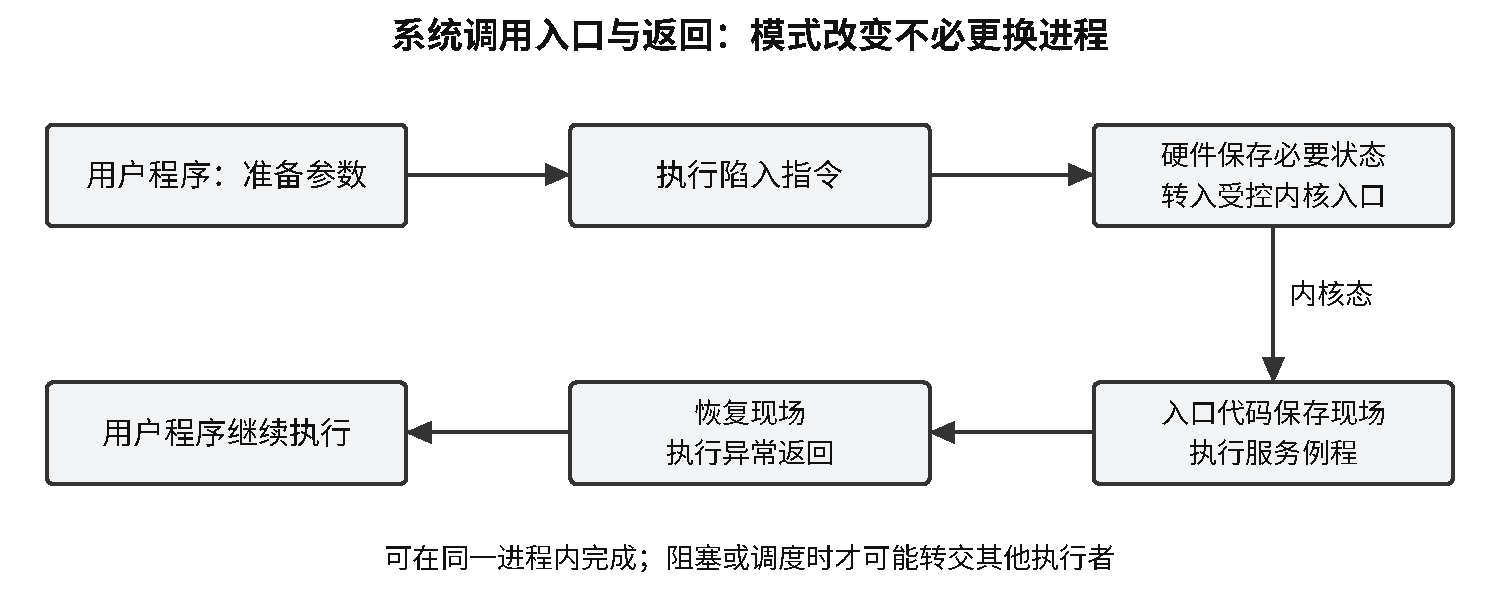
\includegraphics[width=0.94\textwidth,height=\textheight]{figures/OS_control_transfer.pdf}
\caption{从用户程序进入内核，返回时仍可继续原进程}\label{os-fig-control}
\end{figure}

外部中断通常在指令边界被响应；异常通常在指令执行期间被发现。可恢复故障处理完后，可能重新执行产生异常的指令，例如缺页后重试访存；陷入返回通常继续陷入指令的后继指令；不可恢复错误可能终止进程。题目给出具体指令集时，以其断点与返回规则为准。

\subsection{例 1-2　执行系统调用时，哪些操作属于软件}\label{os-ex1-2}

\noindent{}【2022】 执行系统调用的过程涉及下列操作，其中由操作系统完成的是（　）。

Ⅰ. 保存断点和程序状态字　　Ⅱ. 保存通用寄存器的内容

Ⅲ. 执行系统调用服务例程　　Ⅳ. 将 CPU 模式改为内核态

A. 仅Ⅰ、Ⅲ　　B. 仅Ⅱ、Ⅲ　　C. 仅Ⅱ、Ⅳ　　D. 仅Ⅱ、Ⅲ、Ⅳ

\Needspace{6\baselineskip}

\textbf{解析。} 按题目采用的常规异常入口模型，Ⅰ、Ⅳ由响应机制中的硬件完成；Ⅱ由内核入口代码完成，Ⅲ本来就是内核软件执行的服务。因此答案为 \textbf{B}。将模式切换留给不受保护的用户代码会破坏入口的受控性；操作系统不能等自己已经进入服务代码后，才由普通指令任意决定是否取得权限。

中断处理不必导致进程切换。例如时钟中断只更新计数后返回原进程，模式发生了来回变化，但运行者没有改变。这个区别在第2章用于分析上下文切换。

\section{系统调用与库函数：调用一段代码，还是请求内核服务}\label{os-1-5}

\textbf{系统调用}是应用通过规定接口请求内核服务的过程。程序准备调用号和参数，执行陷入指令；内核检查参数、权限及资源状态，分派到相应服务；服务完成或进程以后被唤醒继续时，把结果返回用户程序。检查参数不能省略，例如用户提供的缓冲区地址必须落在允许访问的范围内。

\textbf{库函数}是程序可以调用的已有函数。纯字符串长度计算可以完全在用户态完成；文件读写库函数可能整理格式、维护用户缓冲区，再调用 \texttt{read}、\texttt{write} 等系统调用。因而``调用库函数''既不必然发生模式切换，也不排斥发生系统调用。反过来，系统调用也不是普通函数调用：它跨越保护边界，并通过内核规定的入口执行。

读取磁盘文件时，\texttt{read(fd,}\allowbreak{}\texttt{\ buf,}\allowbreak{}\texttt{\ n)} 中的 \texttt{fd} 标识已经打开的文件，\texttt{buf} 是接收数据的用户缓冲区，\texttt{n} 是请求字节数。若数据已在内核缓存，内核可能复制后直接返回；若必须等待设备，当前进程可能先阻塞，CPU 转去运行其他进程。不要把``系统调用进入内核''与``系统调用必阻塞''合为一条结论。

\noindent{}〖1.1-010〗 库函数不直接处理所有受保护硬件请求。判断一个具体函数是否引起陷入，要看它在本次路径上是否请求内核服务，不能只凭``库函数''这个名称。

\section{从源程序到可运行映像：链接、装入与地址绑定}\label{os-1-6}

编译把源程序翻译为目标模块，目标模块可能仍含未确定的外部符号。\textbf{链接}把多个目标模块和所需库连接起来，解析符号并处理地址引用，形成可装入文件。静态链接在运行前完成所需模块的合并；装入时动态链接在装入时连接；运行时动态链接在首次调用等运行时机连接所需模块。

\textbf{装入}把可执行文件需要的内容映射或读入进程地址空间，并建立运行条件。地址绑定可能发生在不同阶段。

\begin{longtable}[]{@{}
  >{\raggedright\arraybackslash}p{(\columnwidth - 4\tabcolsep) * \real{0.2884}}
  >{\raggedright\arraybackslash}p{(\columnwidth - 4\tabcolsep) * \real{0.3391}}
  >{\raggedright\arraybackslash}p{(\columnwidth - 4\tabcolsep) * \real{0.3723}}@{}}
\toprule\noalign{}
\begin{minipage}[b]{\linewidth}\raggedright
方式
\end{minipage} & \begin{minipage}[b]{\linewidth}\raggedright
地址何时确定
\end{minipage} & \begin{minipage}[b]{\linewidth}\raggedright
移动到另一个物理位置会怎样
\end{minipage} \\
\midrule\noalign{}
\endhead
\bottomrule\noalign{}
\endlastfoot
绝对装入 & 编译或汇编时已给定绝对地址 & 通常须重新生成或修补地址 \\
可重定位装入 & 装入时按实际起点修改相关地址 & 装入后不能仅换一个基址就随意搬移 \\
动态运行时装入/重定位 & 执行访存时由地址变换机构转换 & 更新映射后可改变物理位置，需相应硬件支持 \\
\end{longtable}

最小的动态重定位模型使用基址寄存器 \(B\) 和界限 \(L\)。程序产生逻辑地址 \(a\)，先检查 \(0\le a<L\)，合法时物理地址为 \(B+a\)。例如 \(B=12000,L=2000\)，逻辑地址 1500 转为 13500；逻辑地址 2000 已越界，不能因为``加起来仍在主存里''就放行。界限表示长度时，上界通常不包含；若题目把寄存器定义成最大合法地址，则应按其定义调整比较。

动态重定位在执行阶段进行，依赖重定位信息与硬件地址变换机构，而不是每次访存都调用装入程序。操作系统负责设置和维护映射，硬件完成运行中的快速转换。分页的非连续映射在第5章展开。

\section{进程地址空间中，代码、数据、堆和栈各放什么}\label{os-1-7}

\textbf{地址空间}是一组可由地址标识的位置。进程的虚拟地址空间提供其运行时看到的地址视图，不要求这些地址对应的内容全部同时存在物理内存。可执行文件的磁盘布局、进程的虚拟布局、物理页框布局是三个不同对象。

典型用户空间包含代码区、静态数据区、堆、栈和映射区。代码区存放机器指令，通常只读且可共享；已初始化的全局变量、静态变量通常在初始化数据区，未显式初始化或零初始化的数据可用零填充区表示。堆用于动态申请的对象，栈保存函数活动记录中的参数、返回信息与未被优化掉的自动局部变量。共享库和映射文件可位于映射区。具体地址增长方向和排列由平台决定，示意图不能代替题设。

考虑以下代码，假定采用常规 C 运行时布局且忽略编译优化：

\par\medskip\noindent
\begin{minipage}{\linewidth}
\begin{verbatim}
int g = 3;
static int z;
int main(void) {
    int n = 16;
    char *p = malloc(n);
    /* 使用 p 指向的空间 */
    free(p);
}
\end{verbatim}
\end{minipage}\par\medskip

\texttt{g} 是初始化静态存储期数据，\texttt{z} 是零初始化静态存储期数据；\texttt{n} 和指针变量 \texttt{p} 自身属于 \texttt{main} 的局部活动记录；\texttt{p} 指向的动态对象属于堆。指针存在哪里与它指向的对象存在哪里必须分别回答。不能把``写在函数外''当作``属于代码段''，也不能把所有局部变量都断言为实际驻栈，优化可能把它们放进寄存器或消除。

进程控制块 PCB 保存调度与管理信息，是内核数据结构，不是应用能够随意修改的用户栈对象。同一程序的两个运行实例可以共享只读代码，但具有不同的进程身份、逻辑状态和数据视图。

\section{内核结构：把哪些功能放进同一保护域}\label{os-1-8}

\textbf{分层结构}按依赖关系划分功能，上层使用规定的下层服务，便于逐层验证；代价是层次难划分、调用路径可能增长。\textbf{模块化结构}把功能组织为接口清楚的模块，允许在约定接口下替换实现。模块划分不自动规定严格的层次调用关系，模块也不等于独立的保护域。

\textbf{宏内核}把较多的管理功能放在内核地址空间中，功能间可以直接调用，通信开销较小；一个内核模块的错误也可能影响整个系统。\textbf{微内核}把最基本的调度、低级地址空间管理、进程间通信等保留在内核，把较多服务移到用户态服务器。隔离与替换更容易，但一次服务可能增加消息传递和保护域切换，不能无条件断言性能更好。

\textbf{外核}进一步把资源保护和复用机制与高层资源抽象分开，让应用或库操作系统按需要实现抽象。它并非``没有内核''或``不保护资源''；被保留的保护职责恰是其基础。

比较宏内核与微内核时，先看服务放在哪个保护域，再分析通信和故障如何跨越这个边界。下表比较典型结构；实际系统可以混合采用这些设计。

\begin{longtable}[]{@{}
  >{\raggedright\arraybackslash}p{(\columnwidth - 4\tabcolsep) * \real{0.2520}}
  >{\raggedright\arraybackslash}p{(\columnwidth - 4\tabcolsep) * \real{0.3627}}
  >{\raggedright\arraybackslash}p{(\columnwidth - 4\tabcolsep) * \real{0.3851}}@{}}
\toprule\noalign{}
\begin{minipage}[b]{\linewidth}\raggedright
共同维度
\end{minipage} & \begin{minipage}[b]{\linewidth}\raggedright
宏内核
\end{minipage} & \begin{minipage}[b]{\linewidth}\raggedright
微内核
\end{minipage} \\
\midrule\noalign{}
\endhead
\bottomrule\noalign{}
\endlastfoot
服务的位置 & 文件系统、设备管理等较多服务在内核态 & 只保留基本机制，较多服务由用户态服务器实现 \\
服务间通信 & 同一内核地址空间内可直接调用 & 常经进程间通信、消息传递和保护域切换 \\
故障影响 & 内核模块错误可能破坏其他内核功能 & 用户态服务器的故障较易隔离，但仍需设计恢复机制 \\
扩展和移植 & 模块接口有助维护，修改仍须考虑内核内部依赖 & 可分别调整服务器；小内核较便于验证、移植 \\
性能代价 & 调用路径较短；功能多不等于任意实现都快 & 跨域通信可能增加开销；隔离收益不能直接推出性能更高 \\
\end{longtable}

\subsection{例 1-3　微内核的收益与代价}\label{os-ex1-3}

\noindent{}【2023】 与宏内核操作系统相比，下列特征中，微内核操作系统具有的是（　）。

Ⅰ. 较好的性能　Ⅱ. 较高的可靠性　Ⅲ. 较高的安全性　Ⅳ. 较强的可扩展性

A. 仅Ⅱ、Ⅳ　　B. 仅Ⅰ、Ⅱ、Ⅲ　　C. 仅Ⅰ、Ⅲ、Ⅳ　　D. 仅Ⅱ、Ⅲ、Ⅳ

\Needspace{6\baselineskip}

\textbf{解析。} 服务间保护边界有利于限制故障影响，减少高权限代码有利于安全，服务模块也更容易扩充；但跨域通信会增加开销，不能把Ⅰ列为一般优势。答案为 \textbf{D}。这些是结构层面的比较，不是对任意两个具体系统的性能或安全性作无条件排名。

\section{开机以后，内核怎样获得控制权}\label{os-1-9}

典型引导链为：处理器复位后执行固件中的启动代码，固件初始化必要硬件并选择启动设备；引导程序定位并装入内核；内核建立中断入口、内存管理和设备管理等基本环境，创建初始进程，最后进入正常调度与用户服务。引导程序可以分阶段，早期阶段只装入后续阶段，不能把所有启动代码都理解成同一段磁盘程序。

传统 BIOS/MBR 模型中，磁盘主引导记录可含引导代码和分区表；现代 UEFI/GPT 的组织不同。回答``引导程序在哪里''必须先确定所指的是固件初始代码、主引导代码，还是文件系统中的后续装载器。引导不等于格式化：已经安装的文件系统和分区信息可以跨多次开机保留，而内核运行所需的内存管理结构需要本次启动建立。

\subsection{例 1-4　每次开机需要重新建立什么}\label{os-ex1-4}

\noindent{}【2022】 下列选项中，需要在操作系统进行初始化过程中创建的是（　）。

A. 中断向量表　　B. 文件系统的根目录

C. 硬盘分区表　　D. 文件系统的索引节点表

\Needspace{6\baselineskip}

\textbf{解析。} 中断向量表是本次内核运行所需的控制转移结构，需要在初始化中建立，答案为 \textbf{A}。其余为磁盘格式与文件系统的持久结构，通常在分区或创建文件系统时形成，不应每次开机重建。

\section{虚拟机：客户操作系统也可以成为被管理者}\label{os-1-10}

\textbf{虚拟机管理程序 VMM}向客户操作系统提供虚拟处理器、内存和设备，安排多个虚拟机使用物理资源，并隔离其影响。客户操作系统中的``内核态''是客户的权限视图，不意味着它可以越过 VMM 任意修改主机资源。敏感操作由硬件虚拟化支持、陷入模拟或其他受控机制处理，具体路径随实现变化。

第一类 VMM 直接运行在硬件上；第二类 VMM 依托宿主操作系统运行。二者都可能采用硬件加速，不能简单等同于``硬件实现''和``软件实现''。多台虚拟机可以在单核上交替运行，也可以在多核上并行运行，所以``同时存在多台虚拟机''不能推出它们在每一时刻都真正并行。

进程虚拟地址空间隔离的是进程访存；系统虚拟机为客户操作系统提供完整机器抽象。容器通常共享宿主内核，通过名称空间、资源控制等隔离进程环境，不等同于每个容器都带一个独立客户内核。这里用它帮助辨析抽象层次，不要求记忆容器实现细节。

\section{回顾与自测}\label{os-1-review}

以下为原创回顾设问，用于检查本章机制与边界。

\begin{enumerate}
\def\labelenumi{\arabic{enumi}.}
\tightlist
\item
  普通函数调用、系统调用、设备中断是否都必然更换当前进程？
\item
  用户程序执行陷入指令后进入内核，是否说明陷入指令应禁止在用户态执行？
\item
  基址为 4096、界限为 1024，逻辑地址 1023 与 1024 分别怎样处理？
\item
  指针变量在栈上，是否说明它指向的对象也在栈上？
\item
  单核运行四台虚拟机，是否要求四台同时执行机器指令？
\end{enumerate}

\subsection{自测答案}\label{os-c01-h190}

\begin{enumerate}
\def\labelenumi{\arabic{enumi}.}
\tightlist
\item
  都不必然。函数调用通常不跨保护域；系统调用和设备中断可能只切换模式后返回原进程。只有实际选择另一个执行者才发生相应调度切换。
\item
  否。陷入是用户可执行的受控入口；目标入口和权限变化受硬件及内核规则约束。
\item
  1023 合法，物理地址为 5119；1024 等于长度上界，越界。
\item
  否。须分别判断指针自身与所指对象的生存期和分配方式。
\item
  不要求。它们可以分时复用一个处理器，并发而非同一时刻并行。
\end{enumerate}

\chapter{进程、线程、调度与上下文切换}\label{os-ch2}

程序是指令和数据的静态描述，进程是程序的一次执行过程及其资源环境。同一可执行文件运行两次，可以产生两个进程；同一进程又可以包含多个执行线程。判断状态变化时，要分别问：资源属于谁，当前谁在执行，谁还欠一个事件，谁只是等待处理器。

\section{进程与线程：资源单位和执行单位}\label{os-2-1}

\textbf{进程}是系统进行资源分配和管理的基本单位，具有独立的运行状态和地址空间视图。进程实体通常由程序段、相关数据和进程控制块 PCB 等构成。PCB 记录标识、状态、调度信息、资源使用信息及保存的处理器现场，内核据此管理进程；``一个进程没有正在占用 CPU''不等于它不存在。

\textbf{线程}是进程内部的一条执行流。在引入线程的系统中，处理器调度通常落实到可调度线程，而地址空间、打开文件等资源主要归所属进程。每条线程需要自己的程序计数器、寄存器现场、栈和线程控制信息，否则无法分别记住执行位置和函数调用链。

同一进程的线程可以访问共同的代码、静态数据、堆及进程资源，但拥有独立的执行现场。说``线程有自己的栈''，是说其函数调用状态分别管理，不能据此认为同进程的其他线程在地址上绝对访问不到该栈。只要得到有效地址并具备权限，线程仍可能错误地访问另一线程的对象；私有用途与硬件隔离不同。

进程通常具有动态性、并发性、独立性和异步性。独立性指其运行和管理环境，不表示不能通信或共享；异步性也不允许违反自身指令的必要依赖。线程有利于把服务器中等待网络、处理请求等活动组织成多个执行流，但线程数增加同样会带来同步、栈空间和切换开销。

\begin{longtable}[]{@{}
  >{\raggedright\arraybackslash}p{(\columnwidth - 4\tabcolsep) * \real{0.2577}}
  >{\raggedright\arraybackslash}p{(\columnwidth - 4\tabcolsep) * \real{0.3467}}
  >{\raggedright\arraybackslash}p{(\columnwidth - 4\tabcolsep) * \real{0.3955}}@{}}
\toprule\noalign{}
\begin{minipage}[b]{\linewidth}\raggedright
比较维度
\end{minipage} & \begin{minipage}[b]{\linewidth}\raggedright
不同进程之间
\end{minipage} & \begin{minipage}[b]{\linewidth}\raggedright
同一进程的不同线程之间
\end{minipage} \\
\midrule\noalign{}
\endhead
\bottomrule\noalign{}
\endlastfoot
资源与地址空间 & 各有地址空间和进程资源；共享须按机制建立 & 共享代码、数据、堆和打开文件等所属进程资源 \\
执行现场 & 由各自的控制信息保存 PC、寄存器、栈等 & 每条线程仍有独立 PC、寄存器、栈和线程控制信息 \\
切换要改变什么 & 还需切换相应地址空间环境 & 通常无需更换所属进程的地址空间，仍须换执行现场 \\
数据交换 & 通过共享内存、消息、管道等机制 & 可直接访问共同对象，仍须处理同步与互斥 \\
隔离边界 & 默认地址隔离有助限制误写的影响 & 一个线程可破坏共同空间；自己的栈不等于地址上不可被其他线程访问 \\
\end{longtable}

这里比较的是资源归属；能否由内核分别调度、阻塞是否牵连其他线程，还要看下一节的线程实现与映射模型。

\section{就绪、运行和阻塞：先判断缺少什么}\label{os-2-2}

\textbf{就绪态}表示除处理器外，执行所需条件已满足；\textbf{运行态}表示正在处理器上执行；\textbf{阻塞态}表示等待 I/O、资源、同步事件等条件，暂不能因获得 CPU 就继续。单处理器同一时刻至多一个相应执行实体在运行，就绪与阻塞却都可以有多个。

\begin{figure}
\centering
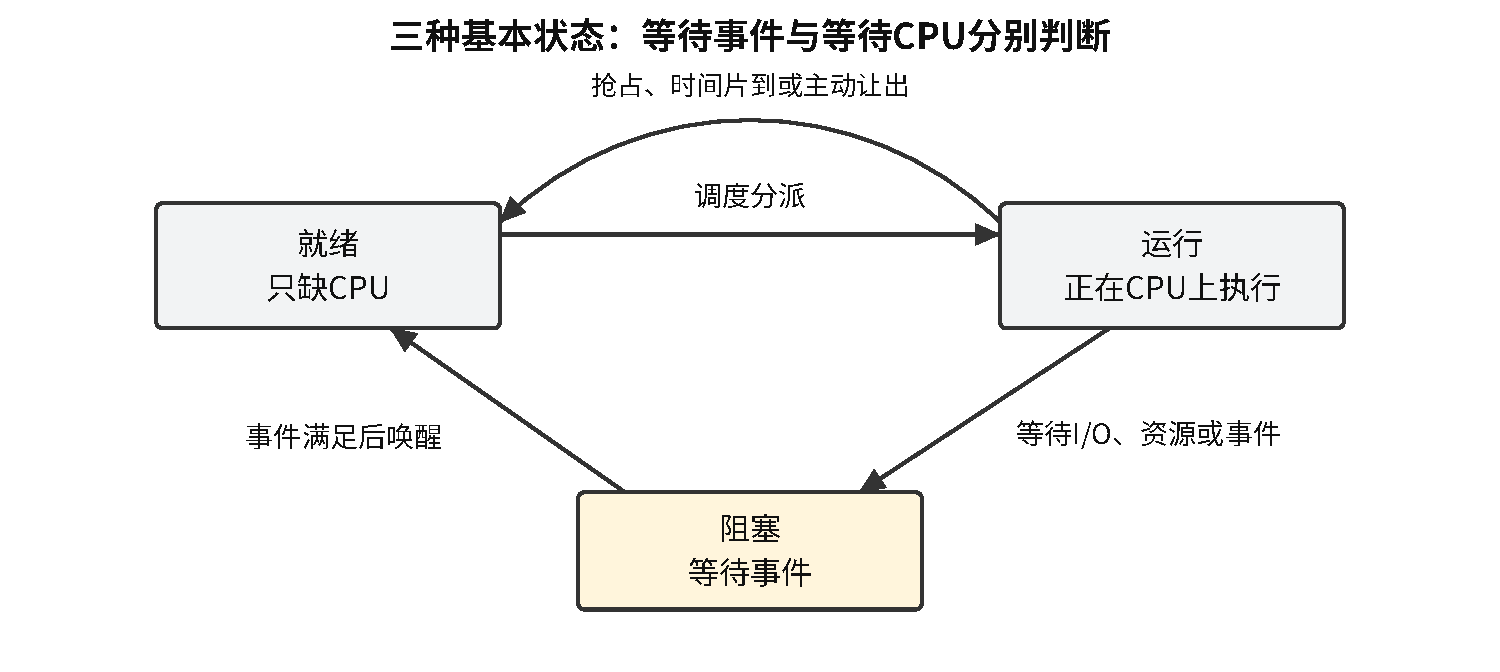
\includegraphics[width=0.94\textwidth,height=\textheight]{figures/OS_process_states.pdf}
\caption{唤醒先进入就绪，调度以后才运行；箭头上的条件不能省略}\label{os-fig-states}
\end{figure}

运行者用完时间片或被更高优先级者抢占，通常转为就绪；执行阻塞式 I/O 而数据未就绪，转为阻塞；等待事件发生后，由内核唤醒为就绪。阻塞者一般不能直接跳到运行，因为事件满足与分配处理器是两个决定。就绪者没有在执行，也不能主动发起一项新的阻塞操作。

创建态用于建立运行环境，终止态用于退出和清理；若进程被换出内存，还可引入挂起就绪、挂起阻塞等状态。挂起表示驻留或管理状态，阻塞表示缺少事件，二者不是同义词。等待事件已满足的挂起阻塞进程，可以先成为挂起就绪，仍须调入并获得 CPU 才能运行。

\subsection{例 2-1　主动让出处理器后去哪里}\label{os-ex2-1}

\noindent{}【2023】 下列由当前线程引起的事件或执行的操作中，可能导致该线程由执行态变为就绪态的是（　）。

A. 键盘输入　　B. 缺页异常　　C. 主动出让 CPU　　D. 执行信号量的 wait() 操作

\Needspace{6\baselineskip}

\textbf{解析。} 主动出让处理器时，线程可能仍具备执行条件，只是把本次运行机会交出去，因而变为就绪，答案为 \textbf{C}。缺页且需等待调页、等待未到来的输入，通常使线程阻塞。信号量 wait 若能取得许可，可继续运行；若不能，则阻塞，而不是仅因调用了 wait 就进入就绪。

键盘输入或另一进程退出临界区，可能满足某个阻塞者等待的条件，使它被唤醒；当前进程的时间片用完则主要改变当前运行者的状态。判断``可能唤醒''时要指明被满足的是哪个等待条件，不能把所有调度事件都当作唤醒。

\section{用户级、内核级线程与映射模型}\label{os-2-3}

\textbf{用户级线程}由用户空间线程库建立和管理，内核可能只看见承载它们的进程或少量内核调度实体。纯用户级线程切换可以只修改用户现场，开销较小；但在多对一模型中，一个承载实体因阻塞式系统调用被阻塞，其他用户线程也失去在该实体上执行的机会；内核也无法把这些用户线程分派到多个核真正并行。

\textbf{内核级线程}由内核识别、管理和调度。某线程阻塞时，同进程的其他内核线程仍可运行；多个线程也可分派到不同核。代价是创建、管理和切换通常需要内核参与，不能把``用户级线程切换开销小''列成内核级线程相对用户级线程的优势。

\begin{longtable}[]{@{}
  >{\raggedright\arraybackslash}p{(\columnwidth - 4\tabcolsep) * \real{0.2917}}
  >{\raggedright\arraybackslash}p{(\columnwidth - 4\tabcolsep) * \real{0.3708}}
  >{\raggedright\arraybackslash}p{(\columnwidth - 4\tabcolsep) * \real{0.3374}}@{}}
\toprule\noalign{}
\begin{minipage}[b]{\linewidth}\raggedright
共同维度
\end{minipage} & \begin{minipage}[b]{\linewidth}\raggedright
用户级线程 ULT
\end{minipage} & \begin{minipage}[b]{\linewidth}\raggedright
内核级线程 KLT
\end{minipage} \\
\midrule\noalign{}
\endhead
\bottomrule\noalign{}
\endlastfoot
谁维护线程控制信息 & 用户空间的线程库 & 操作系统内核 \\
谁选择这一级的运行者 & 线程库选择某个承载实体内的用户线程 & 内核调度器选择可运行的内核线程 \\
切换怎样发生 & 纯用户级切换可只保存、恢复用户现场，不必进入内核 & 由内核保存、恢复相应执行现场并分派 \\
内核能区分到哪一级 & 不能分别调度其不可见的用户线程，只能调度承载实体 & 可分别阻塞、唤醒和分派各内核线程 \\
\end{longtable}

是否牵连其他线程、能否多核并行，还要把这些管理对象按下表映射起来，不能仅凭``用户级''三个字判断所有实现。

\begin{longtable}[]{@{}
  >{\raggedright\arraybackslash}p{(\columnwidth - 4\tabcolsep) * \real{0.2311}}
  >{\raggedright\arraybackslash}p{(\columnwidth - 4\tabcolsep) * \real{0.3515}}
  >{\raggedright\arraybackslash}p{(\columnwidth - 4\tabcolsep) * \real{0.4173}}@{}}
\toprule\noalign{}
\begin{minipage}[b]{\linewidth}\raggedright
映射
\end{minipage} & \begin{minipage}[b]{\linewidth}\raggedright
内核看到什么
\end{minipage} & \begin{minipage}[b]{\linewidth}\raggedright
阻塞和并行的结果
\end{minipage} \\
\midrule\noalign{}
\endhead
\bottomrule\noalign{}
\endlastfoot
多对一 & 多个用户线程对应一个内核执行实体 & 一个阻塞可能挡住全部；不能在多核上同时执行这些用户线程 \\
一对一 & 每个用户线程对应一个内核线程 & 阻塞影响可局部化，可多核并行；内核管理成本较大 \\
多对多 & 多个用户线程复用若干内核线程 & 线程库与内核分层调度，并行度受可用内核线程和核数约束 \\
\end{longtable}

``内核级''描述管理方式，不能理解成该线程的应用代码始终在内核态执行。用户线程进入系统调用时也可能执行内核代码。线程类型、CPU 当前模式、进程所属地址空间是三个不同判断维度。

\section{创建、撤销与组织：PCB 为什么是管理入口}\label{os-2-4}

创建进程一般需要分配标识和 PCB、建立地址空间和初始数据、关联资源、初始化执行现场，再加入适当的调度队列。用户登录、启动程序或系统创建服务进程可能触发创建；给已有进程分配设备只是改变其资源状态，不必产生新进程。

终止进程时，内核停止其执行，处理相关等待与通知，回收资源并释放管理结构。子进程是否随父进程终止，取决于系统的父子关系政策；不能把级联终止当成所有系统的通则。某些系统会保留最少退出信息，供父进程取得状态后再完全释放。

PCB 可以用链表、队列或索引表组织。就绪队列按调度规则组织可运行者，事件等待队列组织等待同类条件者；状态转换时要同步维护状态字段和所在队列。不能只改一个``状态字''而让进程还留在错误队列中。

线程的创建同样要建立 TCB、栈和初始执行现场，但可以复用所属进程的地址空间等资源。在常规父子进程模型中，父子是两个独立进程，可并发执行、有不同 PCB；即使最初采用写时复制暂时共享物理页，也不是共用一个无区分的虚拟地址空间。真正共享的部分须由共享映射等机制说明。

\section{共享内存、消息、管道和信号}\label{os-2-5}

\textbf{共享内存}让多个进程把某些虚拟地址映射到共同的物理存储区。建立映射后，数据交换可以通过普通访存完成，减少反复拷贝；但谁先写、读者何时可读、多个修改者是否冲突，仍需要同步机制。共享内存不自带``不会竞争''的保证。

\textbf{消息传递}把数据交给消息接口，由发送、接收及相关队列组织通信。直接通信指定对方进程，间接通信通过信箱或端口；同步发送、异步发送等语义由接口规定。一次接收若没有消息，可能阻塞，也可能立即报告暂不可用，不能只凭``消息传递''决定状态。

\textbf{管道}提供有次序的数据流通道。经典无名管道常用于有亲缘关系的进程，通常按半双工模型理解；双向通信可用两个管道。命名管道允许按名称建立联系。管道容量有限，空管道上的阻塞读、满管道上的阻塞写都会等待；写入数据后，不代表读取者会立即得到 CPU。

\textbf{信号}是向进程通知某类事件的机制，如终止请求、定时事件等。信号与信号量不同：前者通知事件，后者通过许可计数和等待队列协调资源与次序。普通信号也不等同于携带任意大量数据的可靠消息队列，是否排队等细节须看具体信号类型与接口。

例如父进程经管道把一批数交给子进程：父进程先写数据，子进程读到数据后计算。管道本身组织数据和读写等待；若两者还要更新另一个共享统计量，就仍需为该统计量建立同步保护。不要把``已经用了一种通信方法''推成``所有共享状态都已受保护''。

\section{调度层次与评价指标}\label{os-2-6}

\textbf{高级调度}从后备作业中选作业进入内存并取得参与运行的资格；\textbf{中级调度}通过换出、换入调节内存中的进程数量；\textbf{低级调度}从就绪实体中选择处理器使用者。并非所有现代系统都以经典批处理作业队列呈现三级调度，但三者处理的对象和时间尺度应区分。

设作业或进程 \(i\) 的到达时刻为 \(A_i\)，首次运行时刻为 \(S_i\)，完成时刻为 \(C_i\)，实际服务时间为 \(B_i\)。在只含一个 CPU 段、无 I/O、忽略切换开销的题目中：

\[
T_i=C_i-A_i,\qquad W_i=T_i-B_i,\qquad R_i=S_i-A_i,\qquad T_i^{\mathrm{w}}=\frac{T_i}{B_i}.
\]

\(T_i\) 为周转时间，\(W_i\) 为就绪等待时间，\(R_i\) 为响应时间，\(T_i^{\mathrm{w}}\) 为带权周转时间。平均值是逐个算完再取算术平均；平均带权周转时间一般不等于平均周转时间除以平均运行时间。

若进程有 I/O 等待，周转时间还包含阻塞时间，此时不能只用 \(T_i-B_i\) 当作就绪等待；应再扣除相应阻塞时间。吞吐量是单位时间完成的任务数，CPU 利用率是观察区间内 CPU 忙时长占比。题目是否把切换时间计为``忙''，以及忙于内核开销是否算有效服务，需要按口径说明。

\section{什么时刻可以调度，抢占改变了哪一步}\label{os-2-7}

当前进程结束、主动阻塞或让出处理器，必须考虑选择其他可运行者；新进程到达、I/O 完成使更合适者就绪、时间片到期，也可能触发重新选择。\textbf{非抢占方式}允许当前运行者继续，直到结束或主动放弃；\textbf{抢占方式}允许在满足规则的事件点中断当前运行者，把它放回就绪队列。

调度器负责选择，分派器负责把处理器实际交给所选者，包括必要的现场恢复与切换。发生一次中断不必更换运行者，检查一次调度条件也不等于一定发生进程切换。题目询问``调度次数''时，应核清是否计首次分派、是否计选择原进程、是否计最后转入空闲；不能把事件点数和切换次数混算。

内核维护调度结构的短小临界区等不允许任意抢占，否则可能读到队列的半更新状态；处理中断的阶段也有相应约束。所谓内核可抢占，并非每条内核指令都可以无条件中断并调度。

\section{沿时间线执行调度算法}\label{os-2-8}

处理调度题时，先明确到达时间、服务时间、抢占规则、同刻事件次序及开销。每到一个可能改变选择的事件点，只在\textbf{已经到达且就绪}的进程中选择，记录剩余 CPU 时间。最后用完成时刻计算指标，并检查 CPU 总服务量是否与题表一致。

\subsection{FCFS、SJF、SRTF 与高响应比}\label{os-c02-h116}

\textbf{先来先服务 FCFS}按就绪到达次序选择，通常不抢占。长 CPU 段在前时，后面的短进程和 I/O 型进程可能等很久，产生护航效应。\textbf{短作业/短进程优先 SJF}在选择时挑预计运行时间最短者，通常指非抢占版本；它需要预测运行时间，持续到来的短任务可能使长任务饥饿。

\textbf{最短剩余时间优先 SRTF}是抢占版本，新进程到达时比较的是``新进程的服务时间''与``当前进程剩余时间''，不能拿当前进程最初总时间比较。\textbf{高响应比优先 HRRN}通常非抢占，选择时计算

\[\text{响应比}=\frac{\text{等待时间}+\text{预计服务时间}}{\text{预计服务时间}}=1+\frac{W}{B}.\]

等待越久，响应比越大，有助于缓解长任务长期等候。这个``响应比''是调度优先量，与前节的``响应时间''不是同一个指标。

\subsection{例 2-2　先排除尚未到达者，再比较}\label{os-ex2-2}

\noindent{}【2017】 4 个作业到达系统的时刻和运行时间如下表所示。

\begin{longtable}[]{@{}
  >{\raggedright\arraybackslash}p{(\columnwidth - 4\tabcolsep) * \real{0.3333}}
  >{\raggedright\arraybackslash}p{(\columnwidth - 4\tabcolsep) * \real{0.3333}}
  >{\raggedright\arraybackslash}p{(\columnwidth - 4\tabcolsep) * \real{0.3333}}@{}}
\toprule\noalign{}
\begin{minipage}[b]{\linewidth}\raggedright
作业
\end{minipage} & \begin{minipage}[b]{\linewidth}\raggedright
到达时刻
\end{minipage} & \begin{minipage}[b]{\linewidth}\raggedright
运行时间
\end{minipage} \\
\midrule\noalign{}
\endhead
\bottomrule\noalign{}
\endlastfoot
J1 & 0 & 3 \\
J2 & 1 & 3 \\
J3 & 1 & 2 \\
J4 & 3 & 1 \\
\end{longtable}

系统在 \(t=2\) 时开始作业调度。若分别采用先来先服务和短作业优先调度算法，则选中的作业分别是（　）。

A. J2、J3　　B. J1、J4　　C. J2、J4　　D. J1、J3

\Needspace{6\baselineskip}

\textbf{解析。} 此时只有 J1、J2、J3 到达。FCFS 选择最早到达的 J1；SJF 比较三者运行时间 3、3、2，选择 J3。答案为 \textbf{D}。J4 尚未到达，即使其时间最短也不能提前选择。

\textbf{原创变式。} 沿用本题数据，仅把算法改为 HRRN，检查它与 SJF 是否等同。\(t=2\) 时，J1、J2、J3 的响应比分别为 \(1+2/3\)、\(1+1/3\)、\(1+1/2\)，应选 J1。改变的是优先量，不能仍只比较运行时长。

\subsection{优先级：先看数值方向，再看是否抢占}\label{os-c02-h145}

优先级可以由任务性质静态规定，也可以随等待、CPU 使用等动态调整。数值大代表高还是低，必须按题目读；同为``优先级调度''不保证使用同一方向。提高长等候者优先级称为老化，有助于避免低优先级进程饥饿；实时任务则常需要按紧迫性或期限组织优先次序。

\subsection{例 2-3　被抢占者的剩余时间必须保留}\label{os-ex2-3}

\noindent{}【2023】 进程进入就绪队列的时刻、优先级（值越大优先权越高）及 CPU 执行时间如下表所示。

\begin{longtable}[]{@{}
  >{\raggedright\arraybackslash}p{(\columnwidth - 6\tabcolsep) * \real{0.2415}}
  >{\raggedright\arraybackslash}p{(\columnwidth - 6\tabcolsep) * \real{0.2488}}
  >{\raggedright\arraybackslash}p{(\columnwidth - 6\tabcolsep) * \real{0.2415}}
  >{\raggedright\arraybackslash}p{(\columnwidth - 6\tabcolsep) * \real{0.2681}}@{}}
\toprule\noalign{}
\begin{minipage}[b]{\linewidth}\raggedright
进程
\end{minipage} & \begin{minipage}[b]{\linewidth}\raggedright
到达
\end{minipage} & \begin{minipage}[b]{\linewidth}\raggedright
优先级
\end{minipage} & \begin{minipage}[b]{\linewidth}\raggedright
CPU 时间
\end{minipage} \\
\midrule\noalign{}
\endhead
\bottomrule\noalign{}
\endlastfoot
P1 & 0 ms & 1 & 60 ms \\
P2 & 20 ms & 10 & 42 ms \\
P3 & 30 ms & 100 & 13 ms \\
\end{longtable}

采用基于优先权的抢占式 CPU 调度算法，从 0 ms 开始调度，三个进程的平均周转时间为（　）。

A. 60 ms　　B. 61 ms　　C. 70 ms　　D. 71 ms

\begin{figure}
\centering
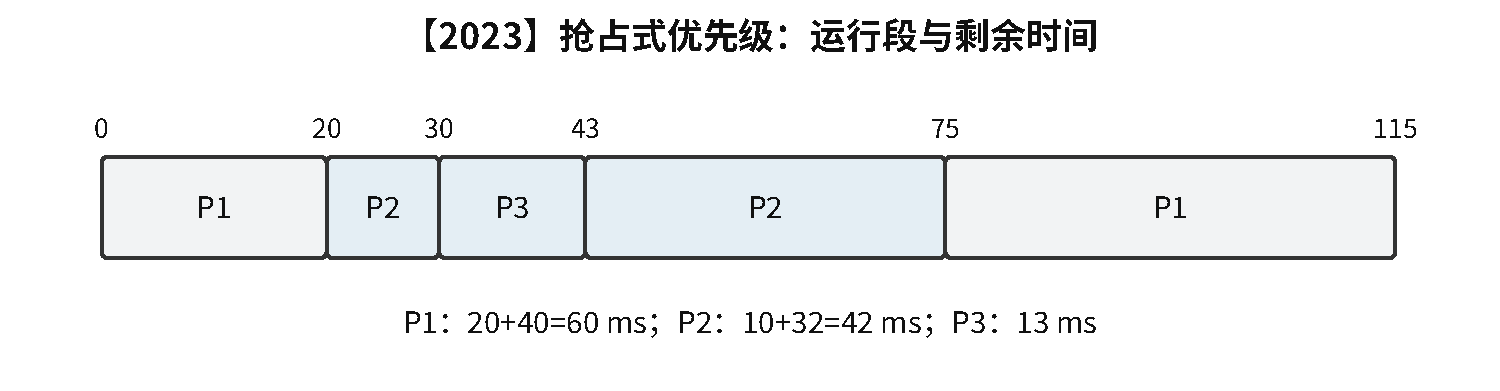
\includegraphics[width=0.96\textwidth,height=\textheight]{figures/OS_priority_timeline.pdf}
\caption{每次抢占保留剩余时间，不重新开始整个 CPU 段}\label{os-fig-priority}
\end{figure}

\Needspace{6\baselineskip}

\textbf{解析。} 0---20 ms 只有 P1，执行 20 ms 后还余 40 ms。P2 到达并抢占，执行至 30 ms，还余 32 ms。P3 优先级最高，30---43 ms 执行完毕；随后 P2 执行 32 ms，于 75 ms 完成；最后 P1 执行 40 ms，于 115 ms 完成。

三者周转时间依次为 \(115-0=115\) ms、\(75-20=55\) ms、\(43-30=13\) ms，平均为 \((115+55+13)/3=61\) ms，答案为 \textbf{B}。完成时刻之和不是周转时间之和；每项都要减各自到达时刻。

\subsection{例 2-4　一次到达不必增加一次进程调度}\label{os-ex2-4}

\noindent{}【2022】 P0、P1、P2、P3 的到达、优先级（值越小优先权越高）和执行时间如下表所示。采用基于优先权的抢占式进程调度，从 0 ms 开始，到四个进程都运行结束为止，发生进程调度的总次数为（　）。

\begin{longtable}[]{@{}
  >{\raggedright\arraybackslash}p{(\columnwidth - 6\tabcolsep) * \real{0.2410}}
  >{\raggedright\arraybackslash}p{(\columnwidth - 6\tabcolsep) * \real{0.2495}}
  >{\raggedright\arraybackslash}p{(\columnwidth - 6\tabcolsep) * \real{0.2410}}
  >{\raggedright\arraybackslash}p{(\columnwidth - 6\tabcolsep) * \real{0.2682}}@{}}
\toprule\noalign{}
\begin{minipage}[b]{\linewidth}\raggedright
进程
\end{minipage} & \begin{minipage}[b]{\linewidth}\raggedright
到达
\end{minipage} & \begin{minipage}[b]{\linewidth}\raggedright
优先级
\end{minipage} & \begin{minipage}[b]{\linewidth}\raggedright
CPU 时间
\end{minipage} \\
\midrule\noalign{}
\endhead
\bottomrule\noalign{}
\endlastfoot
P0 & 0 ms & 15 & 100 ms \\
P1 & 10 ms & 20 & 60 ms \\
P2 & 10 ms & 10 & 20 ms \\
P3 & 15 ms & 6 & 10 ms \\
\end{longtable}

A. 4　　B. 5　　C. 6　　D. 7

\Needspace{6\baselineskip}

\textbf{解析。} 实际运行段依次为 P0{[}0,10)、P2{[}10,15)、P3{[}15,25)、P2{[}25,40)、P0{[}40,130)、P1{[}130,190)。P1 在 10 ms 到达，但优先级低于当时可选者，不单独取得一个运行段。按题目计首次分派且不计最后转入空闲，六次分派，答案为 \textbf{C}。若只数相邻两个实际运行进程的更换，则是五次；两种口径不可混用。

\subsection{时间片轮转与多级反馈队列}\label{os-c02-h184}

\textbf{时间片轮转 RR}让就绪队列按先后取得至多一个时间片。进程在时间片内结束或阻塞，就提前让出；用完时间片仍未结束者回到队尾。时间片过长会接近 FCFS，过短会增加切换开销。若每次有效执行 \(q\)、切换耗时 \(s\)，持续满负荷时有效服务占比可近似写为 \(q/(q+s)\)，但最后一个短段等边界应逐段算。

同刻有新进程到达又有时间片到期时，谁先入队可能改变结果，应按题设；题设没有规定且确实影响答案时，必须声明采用的次序。不能把刚被抢占的进程总放在队首，也不能让新来者跳过当前时间片。

\textbf{多级队列}把不同类型进程固定放在不同队列；\textbf{多级反馈队列}允许进程在队列间移动，常用较高队列的短时间片及时响应交互，CPU 使用较长者逐级下降。队列间是否抢占、各级规则和提升规则必须逐项读取，不能靠一个固定代码模板代替题设。

\subsection{例 2-5　二级反馈中，第二级按剩余量选择}\label{os-ex2-5}

\noindent{}【2019】 系统采用二级反馈队列调度。Q1 采用时间片轮转，时间片为 10 ms；Q2 采用短进程优先。系统优先调度 Q1，Q1 为空才调度 Q2；新创建进程先进入 Q1，在 Q1 执行一个时间片后仍未结束则转入 Q2。当前两队列为空，系统依次创建 P1、P2 后开始调度，两者需要的 CPU 时间分别为 30 ms、20 ms。平均等待时间为（　）。

A. 25 ms　　B. 20 ms　　C. 15 ms　　D. 10 ms

\Needspace{6\baselineskip}

\textbf{解析。} P1 在 Q1 执行 0---10 ms，余 20；P2 执行 10---20 ms，余 10。此时 Q1 为空，Q2 中 P2 剩余较短，先执行 20---30 ms 完成，再运行 P1 至 50 ms。两者初始时均已创建，等待分别为 \(50-30=20\) ms、\(30-20=10\) ms，平均 15 ms，答案为 \textbf{C}。转入 Q2 以后，已经执行的时间不能重复计算。

\subsection{例 2-6　同一组到达事件，SRTF 与 RR 如何分别推进}\label{os-ex2-6}

\noindent{}〖2.2-006〗 系统有 4 个进程，预计运行时间和到达就绪队列的时刻如下，单位均为时间配额。分别采用可抢占式短进程优先和时间片轮转调度（时间片为 2），求各进程的调度次序与平均周转时间。

\begin{longtable}[]{@{}
  >{\raggedright\arraybackslash}p{(\columnwidth - 4\tabcolsep) * \real{0.3253}}
  >{\raggedright\arraybackslash}p{(\columnwidth - 4\tabcolsep) * \real{0.3253}}
  >{\raggedright\arraybackslash}p{(\columnwidth - 4\tabcolsep) * \real{0.3493}}@{}}
\toprule\noalign{}
\begin{minipage}[b]{\linewidth}\raggedright
进程
\end{minipage} & \begin{minipage}[b]{\linewidth}\raggedright
到达时刻
\end{minipage} & \begin{minipage}[b]{\linewidth}\raggedright
预计运行时间
\end{minipage} \\
\midrule\noalign{}
\endhead
\bottomrule\noalign{}
\endlastfoot
P1 & 0 & 8 \\
P2 & 1 & 4 \\
P3 & 2 & 9 \\
P4 & 3 & 5 \\
\end{longtable}

\Needspace{6\baselineskip}

\textbf{解析。} SRTF 在 0 时先选 P1；到 1 时 P1 余 7，而 P2 只需 4，故抢占。到 2 时 P2 余 3，小于新来的 P3 的 9；到 3 时 P2 余 2，小于 P4 的 5，均不抢占。P2 在 5 完成后，等待者的剩余量依次为 P1 的 7、P3 的 9、P4 的 5，因此先 P4，再 P1，最后 P3。

\begin{longtable}[]{@{}
  >{\raggedright\arraybackslash}p{(\columnwidth - 4\tabcolsep) * \real{0.2963}}
  >{\raggedright\arraybackslash}p{(\columnwidth - 4\tabcolsep) * \real{0.4073}}
  >{\raggedright\arraybackslash}p{(\columnwidth - 4\tabcolsep) * \real{0.2963}}@{}}
\toprule\noalign{}
\begin{minipage}[b]{\linewidth}\raggedright
进程
\end{minipage} & \begin{minipage}[b]{\linewidth}\raggedright
SRTF 实际运行区间
\end{minipage} & \begin{minipage}[b]{\linewidth}\raggedright
周转时间
\end{minipage} \\
\midrule\noalign{}
\endhead
\bottomrule\noalign{}
\endlastfoot
P1 & {[}0,1)、{[}10,17) & 17 \\
P2 & {[}1,5) & 4 \\
P3 & {[}17,26) & 24 \\
P4 & {[}5,10) & 7 \\
\end{longtable}

平均周转为 \((17+4+24+7)/4=13\)。P3、P4 到达都使调度器重新比较，但比较后可以继续当前 P2，不能把每次到达都强制切换。

RR 按本题参考解采用``同刻新到者先入队，再把时间片到期者放队尾''的约定。P1 在 {[}0,2) 后回队尾，此时队列为 P2、P3、P1；P4 在 3 到达，排在当时的等待队尾。以后按同样规则，每次只扣实际使用的一个时间片；剩余不足 2 者提前结束。

\begin{longtable}[]{@{}
  >{\raggedright\arraybackslash}p{(\columnwidth - 4\tabcolsep) * \real{0.2600}}
  >{\raggedright\arraybackslash}p{(\columnwidth - 4\tabcolsep) * \real{0.4780}}
  >{\raggedright\arraybackslash}p{(\columnwidth - 4\tabcolsep) * \real{0.2618}}@{}}
\toprule\noalign{}
\begin{minipage}[b]{\linewidth}\raggedright
进程
\end{minipage} & \begin{minipage}[b]{\linewidth}\raggedright
RR 实际运行区间
\end{minipage} & \begin{minipage}[b]{\linewidth}\raggedright
周转时间
\end{minipage} \\
\midrule\noalign{}
\endhead
\bottomrule\noalign{}
\endlastfoot
P1 & {[}0,2)、{[}6,8)、{[}14,16)、{[}20,22) & 22 \\
P2 & {[}2,4)、{[}10,12) & 11 \\
P3 & {[}4,6)、{[}12,14)、{[}18,20)、{[}23,25)、{[}25,26) & 24 \\
P4 & {[}8,10)、{[}16,18)、{[}22,23) & 20 \\
\end{longtable}

平均周转为 \((22+11+24+20)/4=19.25\)。最后只有 P3，它在 25 用完一个片后仍可再次获选，不能因为``轮转''而强行等待一个不存在的其他进程。若同刻入队约定改变，2 时的队列及以后轨迹也要随之重算。

\subsection{调度算法的选择依据与抢占条件}\label{os-c02-h233}

下表比较的是前述 CPU 调度规则。``需要时长''指选择时需要已知或估计的 CPU 服务量，不是说运行时间必须由用户准确预报。各种算法都只在已到达、已就绪的实体中选择。

\begin{longtable}[]{@{}
  >{\raggedright\arraybackslash}p{(\columnwidth - 8\tabcolsep) * \real{0.1721}}
  >{\raggedright\arraybackslash}p{(\columnwidth - 8\tabcolsep) * \real{0.2029}}
  >{\raggedright\arraybackslash}p{(\columnwidth - 8\tabcolsep) * \real{0.1901}}
  >{\raggedright\arraybackslash}p{(\columnwidth - 8\tabcolsep) * \real{0.1959}}
  >{\raggedright\arraybackslash}p{(\columnwidth - 8\tabcolsep) * \real{0.2388}}@{}}
\toprule\noalign{}
\begin{minipage}[b]{\linewidth}\raggedright
算法
\end{minipage} & \begin{minipage}[b]{\linewidth}\raggedright
下一个运行者怎样选
\end{minipage} & \begin{minipage}[b]{\linewidth}\raggedright
是否抢占
\end{minipage} & \begin{minipage}[b]{\linewidth}\raggedright
是否需要预计 CPU 时长
\end{minipage} & \begin{minipage}[b]{\linewidth}\raggedright
等待方面的主要边界
\end{minipage} \\
\midrule\noalign{}
\endhead
\bottomrule\noalign{}
\endlastfoot
FCFS & 按进入就绪队列的先后 & 通常不抢占 & 不需要 & 正常推进时不因后到者插队而饥饿；短任务可能被长任务拖住 \\
SJF & 预计服务时间最短者 & 本章指非抢占版 & 需要预计服务时间 & 持续到来的短任务可能使长任务饥饿 \\
SRTF & 预计剩余时间最短者 & 可以抢占 & 需要预计剩余时间 & 比较剩余量；持续短任务同样可能阻挡长任务 \\
HRRN & 选择 \(1+W/B\) 最大者 & 通常不抢占 & 需要预计服务时间 \(B\) & 等待使响应比增加，兼顾长短任务；不等于固定等待上界 \\
优先级 & 按题设优先级高低 & 两种版本都有 & 通常不以时长为必需输入 & 固定低优先级者可能饥饿；老化可逐步提高其优先级 \\
RR & 队首运行至片满、结束或阻塞 & 片满时抢占 & 不需要 & 同队列轮流获得机会；片过小会增加切换开销 \\
多级反馈队列 & 先选队列，再执行该队列规则 & 常见模型允许高队列抢占 & 不需事先估计总服务时间 & 若高队列始终有任务，低队列可能长期无机会；是否定期提升须看规则 \\
\end{longtable}

``短任务优先''不自动包含抢占；``按优先级''也不自动包含时间片。题干同时给出多个规则时，先判断哪个规则决定候选队列，再判断队内顺序，最后处理到达、片满和阻塞等事件。

\subsection{例 2-7　把``等待越久越优先''写成动态优先数}\label{os-ex2-7}

\noindent{}【2016】 某进程调度程序采用基于优先数（priority）的调度策略，即选择优先数最小的进程运行。进程创建时由用户指定一个 nice 作为静态优先数。为了动态调整优先数，引入运行时间 cpuTime 和等待时间 waitTime，初值均为 0。进程处于执行态时，cpuTime 定时加 1，且 waitTime 置 0；进程处于就绪态时，cpuTime 置 0，waitTime 定时加 1。请回答下列问题。

（1）若调度程序只将 nice 的值作为进程的优先数，即 priority=nice，则可能会出现饥饿现象，为什么？

（2）使用 nice、cpuTime 和 waitTime 设计一种动态优先数计算方法，以避免产生饥饿现象，并说明 waitTime 的作用。

\Needspace{6\baselineskip}

\textbf{解析。} （1）数值小才优先。若就绪队列中一直有 nice 较小的进程，nice 较大的进程便可能一直落选。系统仍有其他进程在运行，因此这是饥饿，不能解释成全部进程互等的死锁。

（2）一种方法是

\[priority=nice+k_1\,cpuTime-k_2\,waitTime,\qquad k_1>0,\ k_2>0.\]

运行时间增长使优先数增大，降低持续占用 CPU 者的优先级；就绪等待增长使优先数减小，提高长期等待者的优先级。两个符号都由``数值越小越优先''决定，不能沿用数值越大越优先的公式。

例如仅为检验公式方向，取 \(k_1=k_2=1\)：nice=10 的等待者在等待 11 个计时单位后，优先数成为 −1，可以超过 nice=0、刚就绪的进程。这是\textbf{原创代入检查}，不是原题新增数据。等待者一旦运行，waitTime 按题设清零；再次就绪时 cpuTime 清零，不能把这两个量误当成从创建起永久累计的总量。

waitTime 提供的是老化机制。将它用作无饥饿保证，还需采用通常的有限进程或有界 nice 模型、持续计时和重算、适当抢占或有限运行段，以及同优先数下不无限越过等待者等条件；不能把一个公式解释成对任意到达流和任意调度实现都存在固定等待上界。

\section{多处理机调度：负载与缓存都有代价}\label{os-2-9}

多个处理器可以使用公共就绪队列，也可以各自维护队列。公共队列便于共享负载，但并发访问需同步；每核队列降低争用，却可能出现一核排队、一核空闲，需要负载均衡。推迁移由繁忙者把任务移出，拉迁移由空闲者取得任务。

\textbf{处理器亲和性}倾向让线程继续在此前运行的处理器上执行，利用缓存和地址转换缓存中的内容。软亲和性是调度倾向，硬亲和性是允许处理器集合的明确限制。负载均衡可能要求迁移，缓存局部性可能要求保留，二者需要权衡；不能把``每核进程数相同''当作负载完全相同，因为各任务剩余计算量可能不同。

同时多线程 SMT 让一个物理核维护多个硬件线程现场，共享某些执行资源；它不等于每条逻辑处理器都具有独立完整的执行单元。调度题未给多处理机规则时，不要自行把一个进程拆到多个核同时加速。

\section{上下文切换与模式切换}\label{os-2-10}

\textbf{上下文}是恢复执行所需的状态，包括程序计数器、寄存器、栈等；进程切换还可能更换地址空间相关状态。\textbf{模式切换}只是当前执行权限模式改变，例如同一进程进入系统调用再返回；它不必改变执行身份。\textbf{上下文切换}则把 CPU 从一个执行实体交给另一个。

同进程的线程切换通常要换 PC、寄存器和栈，而不必更换进程页表基址和共同的文件资源。跨进程切换还要建立新地址空间环境；TLB 是否必须全部清空，取决于是否支持地址空间标识等硬件条件。不能把``跨进程切换一定清空全部 Cache''列作一般步骤。

\noindent{}〖2.2-009〗 同一进程中 T1 切到 T2，需要更新各自执行位置和栈环境；进程页表和进程打开文件资源并不因同进程线程切换而自然改变。判断题列出的每项寄存器，要先说明它保存线程状态还是进程共享状态。

\noindent{}【2023】 ``执行系统调用''完成并返回调用者时，可以使 CPU 从内核态回到用户态；阻塞、唤醒和执行 CPU 调度本身属于内核管理路径，不能把它们的完成都理解成必然返回用户态。具体返回到哪个线程，由当时调度与返回路径决定。

\section{自测：用相同时间线检查不同问题}\label{os-2-review}

以下为原创回顾设问。

\begin{enumerate}
\def\labelenumi{\arabic{enumi}.}
\tightlist
\item
  已等到 I/O 数据的进程是否立即运行？线程发出 I/O 请求是否必然阻塞？
\item
  在例2-3中，P2 的响应时间、等待时间、周转时间分别是多少？
\item
  同一进程的两个内核线程切换，是否必须改页表基址？
\item
  预计服务时间相同的两个作业，HRRN 如何反映等待差别？
\item
  多核上迁移线程，一定能提高性能吗？
\end{enumerate}

\subsection{自测答案}\label{os-c02-h297}

\begin{enumerate}
\def\labelenumi{\arabic{enumi}.}
\tightlist
\item
  数据到达使相应等待条件满足，通常先就绪，再等调度。若请求非阻塞或数据已可用，I/O 接口可不使线程阻塞。
\item
  P2 在到达 20 ms 时立即开始，响应时间 0；周转时间 55 ms，服务 42 ms，所以等待 13 ms。
\item
  通常不必，二者使用同一进程地址空间，但 PC、寄存器和线程栈等要切换。
\item
  \(B\) 相同则 \(1+W/B\) 随 \(W\) 增大，等待较久者响应比更高。
\item
  不一定。迁移可能缓解排队，也可能丢失缓存局部性、产生同步和迁移成本。
\end{enumerate}

\chapter{同步、互斥与信号量}\label{ch-sync}

进程合作时，需要回答两个不同的问题：一项操作必须等谁完成，几个进程能否同时操作同一份共享数据。前者决定先后次序，后者决定互斥范围。信号量可以表达这两种约束，但其含义、初值和放置位置都要从题目条件推出。

本章代码是描述并发关系的伪代码。\texttt{P(S)} 与 \texttt{wait(S)} 同义，\texttt{V(S)} 与 \texttt{signal(S)} 同义；条件变量的 \texttt{wait}、\texttt{signal} 会另行定义。进程编号与数组下标从 0 开始。除特别说明，信号量采用本章的记录型语义，不假定等待队列按先进先出调度。

\section{临界区约束什么，为什么还需要同步}\label{sec-concepts}

\subsection{从一次丢失的更新看原子操作}\label{os-c03-h9}

两个进程共享整数 \texttt{x}，初值为 0，各执行一次 \texttt{x=x+1}。一条高级语言语句未必是一条不可分割的机器操作。若每次更新分为``读入本地寄存器---加 1---写回''，就可能出现下图的交错：两个进程都读到 0，最后都写入 1，结果只有 1。

\begin{figure}
\centering
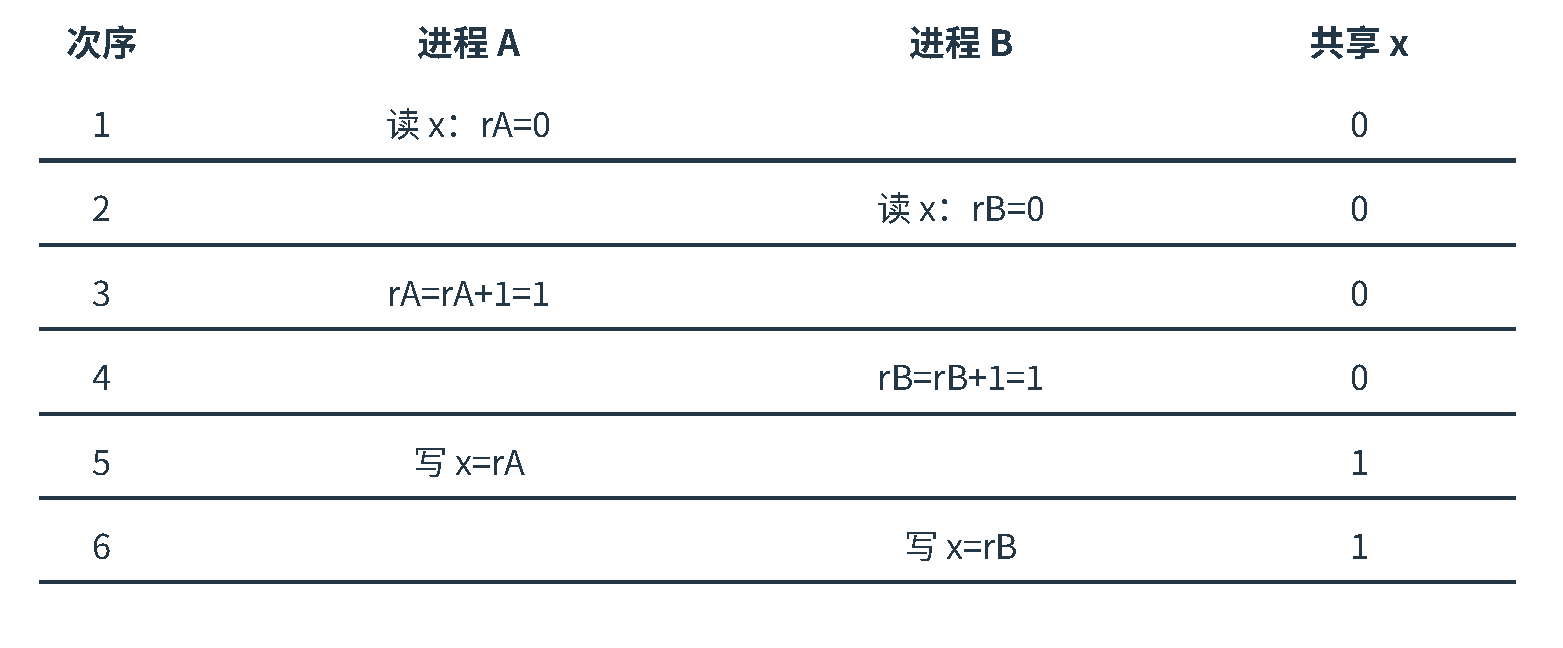
\includegraphics[width=0.94\textwidth,height=\textheight]{figures/F01_lost_update.pdf}
\caption{两次更新都完成，但后一次写回覆盖了前一次结果}\label{fig-lost}
\end{figure}

即使只有一个 CPU，进程也可能在读与写之间被切换出去，所以单处理机不能免除竞争。多处理机上还可能真正同时执行。这里把某段操作视为\textbf{原子操作}，是说其他并发操作不能在其内部插入并观察到破坏该操作语义的中间状态；不能仅凭``这是一行代码''认定原子性。

进程在运行态时占用处理机；在就绪态时具备运行条件，等待调度；在阻塞态时等待事件，暂时不能被调度执行。因资源不足而主动阻塞，与反复执行检查指令的忙等待不同。唤醒把阻塞进程变为就绪进程，不保证它立即运行。

\subsection{资源、代码与先后关系}\label{os-c03-h19}

\textbf{临界资源}是在同一时段只允许一个进程使用的共享资源。\textbf{临界区}是进程中访问相应临界资源的代码段。进入区负责申请进入，退出区负责释放；二者不属于被保护的临界区本身。资源是一份共享对象，相关临界区可以有多段，分布在不同进程中。

\noindent{}〖2.3-027〗 5 个并发进程各有一段访问同一变量 A 的代码，对应 5 个相关临界区。一份共享变量不能代替五段代码来计数。一般程序若有多处访问，不能仅凭进程数推出代码段总数。

\textbf{互斥}限制重叠：某进程正在访问临界资源时，其他需要访问它的进程须等待。\textbf{同步}规定合作中的先后关系：后续操作需要某项结果，就必须等产生该结果的操作完成。同一对进程可能同时受这两种约束。

\subsection{例 3-1　共享缓冲区中的两种约束}\label{ex-err11}

\noindent{}〖2.3-011〗 进程 A 和进程 B 通过共享缓冲区协作完成数据处理，进程 A 负责产生数据并放入缓冲区，进程 B 从缓冲区读数据并输出。进程 A 和进程 B 之间的制约关系是（　）。

A. 互斥关系　　B. 同步关系　　C. 互斥和同步关系　　D. 无制约关系

\Needspace{6\baselineskip}

\textbf{解析。} B 必须在 A 放入数据后读取，这是同步；对共享缓冲区的访问还须协调，避免操作冲突，这是互斥。答案为 \textbf{C}。B 只表达了先后约束。

本题指出两类约束，并不意味着任何实现都必须恰好使用``一个同步量加一个互斥量''。操作是否反复执行、容量是否为 1，以及同步本身是否已排除重叠，都会影响实现；\hyperref[ex-2024]{例3-4}会分别处理。

\subsection{怎样判断互斥方案是否合格}\label{os-c03-h37}

检查一种方案时，先找违反条件的具体交错，不要只看顺序执行的结果。

\begin{longtable}[]{@{}
  >{\raggedright\arraybackslash}p{(\columnwidth - 2\tabcolsep) * \real{0.3163}}
  >{\raggedright\arraybackslash}p{(\columnwidth - 2\tabcolsep) * \real{0.6836}}@{}}
\toprule\noalign{}
\begin{minipage}[b]{\linewidth}\raggedright
检查项
\end{minipage} & \begin{minipage}[b]{\linewidth}\raggedright
要问的问题
\end{minipage} \\
\midrule\noalign{}
\endhead
\bottomrule\noalign{}
\endlastfoot
空闲让进 & 临界区无人使用，是否仍被一个不参与竞争的进程挡住？ \\
忙则等待 & 一个进程尚未退出，另一个能否进入同一临界区？ \\
有限等待 & 请求提出后，其他进程获准进入的次数是否存在有限上界？还须满足进程持续获得执行机会、临界区操作有限等前提。 \\
让权等待 & 不能进入时，是阻塞并让出处理机，还是继续占用 CPU 检查？ \\
\end{longtable}

前三项分别检查进入机会、互斥安全和等待上界；让权等待检查等待方式。一个自旋方案可能保证互斥，却不满足让权等待。\textbf{无死锁也不自动意味着无饥饿}：系统仍有进程前进，但某个进程可能反复被越过。

\section{软件互斥与锁：检查和占用必须连起来}\label{sec-locks}

\subsection{三种失败方案留下了什么问题}\label{os-c03-h52}

以下双进程模型假定单次共享变量读写原子、内存顺序与伪代码一致。\texttt{flag{[}i{]}} 表示进程 \(P_i\) 想进入。现代机器上的编译器和存储重排不在这些伪代码的默认模型内，实际程序还需相应原子变量与内存序保证。

\begin{longtable}[]{@{}
  >{\raggedright\arraybackslash}p{(\columnwidth - 4\tabcolsep) * \real{0.2437}}
  >{\raggedright\arraybackslash}p{(\columnwidth - 4\tabcolsep) * \real{0.3278}}
  >{\raggedright\arraybackslash}p{(\columnwidth - 4\tabcolsep) * \real{0.4283}}@{}}
\toprule\noalign{}
\begin{minipage}[b]{\linewidth}\raggedright
方案
\end{minipage} & \begin{minipage}[b]{\linewidth}\raggedright
进入区的核心操作
\end{minipage} & \begin{minipage}[b]{\linewidth}\raggedright
一条足以否定它的执行情况
\end{minipage} \\
\midrule\noalign{}
\endhead
\bottomrule\noalign{}
\endlastfoot
单标志法 & 等待 \texttt{turn==i}，退出时将机会交给对方 & \texttt{turn=0}，但 \(P_0\) 一直做剩余区（不访问该临界资源的其他代码）工作；\(P_1\) 不能进入空闲临界区。 \\
双标志先检查 & 先等对方 \texttt{flag} 为假，再置自己为真 & 双方都在对方置真前完成检查，随后同时进入，不能保证互斥。 \\
双标志后检查 & 先置自己为真，再等对方为假 & 双方先置真，都等待对方退出；此时没有任何一方进入，无法执行清标志。 \\
\end{longtable}

这些模型与反例见王道书 §2.3。先检查法的问题是``检查与声明占用分离''；简单调换两句又可能造成双方互等。

\subsection{Peterson 算法怎样处理双方同时申请}\label{os-c03-h64}

Peterson 算法用 \texttt{flag} 表达意愿，用 \texttt{turn} 在双方都想进入时决定让谁先走。两个 \texttt{flag} 初值均为 \texttt{false}；对 \(i\in\{0,1\}\)，令 \(j=1-i\)：

\par\medskip\noindent
\begin{minipage}{\linewidth}
\begin{verbatim}
flag[i] = true;
turn = j;
while (flag[j] && turn == j) { }  // 忙等待
访问临界资源;
flag[i] = false;
\end{verbatim}
\end{minipage}\par\medskip

若只有自己请求，对方的 \texttt{flag} 为假，可直接进入。若双方都请求，两次对 \texttt{turn} 的写入总有先后；最后把机会让给对方的进程等待，另一方可进入。退出时清除自己的意愿，等待者随后通过检查。

还须排除``一个已进入，另一个又进来''的情况。假设 \(P_i\) 在临界区，故 \texttt{flag{[}i{]}} 为真；后来的 \(P_j\) 声明意愿并将 \texttt{turn} 置为 \texttt{i}，就必须等待。如果双方已在进入区竞争，后一次 \texttt{turn} 写入同样使其中一方等候。由此排除同时进入。在上述内存模型、进程继续执行且临界区有限等前提下，它也能保证有限等待；它仍在循环检查，不能让权等待。

\subsection{TestAndSet 为什么能够上锁}\label{os-c03-h80}

硬件提供的 TestAndSet（TS，也称 TSL）以一次原子操作返回 \texttt{lock} 的旧值，并把 \texttt{lock} 置为真。以下只是该指令的逻辑含义，不能把普通语言实现的三句代码直接当作原子指令：

\par\medskip\noindent
\begin{minipage}{\linewidth}
\begin{verbatim}
TestAndSet(lock):
    old = lock
    lock = true
    return old

// lock 初值 false
while (TestAndSet(lock)) { }
访问临界资源;
lock = false;
\end{verbatim}
\end{minipage}\par\medskip

第一个读到假值的调用者同时把锁置真；后续调用者得到真值，继续等待。关键是``取旧值并置真''不可被其他竞争者插入，而不是 \texttt{while} 语句本身有特殊能力。Swap/XCHG 则原子交换共享的 \texttt{lock} 与进程私有的 \texttt{key}。共享 \texttt{lock} 初值为假，每次申请先令本进程的 \texttt{key=true}，再反复原子交换二者，直到 \texttt{key=false}，表示取得了交换前的空闲锁；退出时令 \texttt{lock=false}。

这类锁若一直循环，就是\textbf{自旋锁}。它避免睡眠和唤醒的切换开销，适用于持锁时间很短、持锁者能够继续运行的情形。它不保证公平，不能只从指令原子性推出有限等待。阻塞锁在不可用时使线程睡眠，更适合可能较长的等待；不能把``互斥锁''一词一概等同于自旋实现。

单处理机上，自旋者正在运行时，持锁者不能同时运行；若调度还能让持锁者重新运行，锁仍可能被释放。若相关内核区又禁止了能让持锁者运行的切换，便不能指望忙等自行结束。多处理机上，其他核可继续执行持锁者。

屏蔽本 CPU 的可屏蔽中断，只能在单处理机、相关执行路径不会主动阻塞等限定下保护短小的内核临界操作；它不能阻止另一 CPU 访问共享数据，不能用作一般多处理机互斥。开关中断是特权操作，也不能交给普通用户程序任意使用。分析原语的原子性时，应说明保护范围，不能笼统写``所有原语都靠关中断''。

\section{信号量：先说明它代表什么，再计算初值}\label{sec-semaphore}

\subsection{记录型 P、V 的完整语义}\label{os-c03-h106}

记录型信号量 \(S\) 包含整数 \texttt{value} 与等待队列。初始化只做一次；以后通过 P、V 改变状态。以下``修改计数---判断---入队或唤醒''须由系统作为原子同步操作实现；进程阻塞后并不把整个等待期间变成不可调度的原子区。

\par\medskip\noindent
\begin{minipage}{\linewidth}
\begin{verbatim}
P(S):
    S.value = S.value - 1
    if S.value < 0:
        将当前进程加入 S 的等待队列并阻塞
        // 被唤醒后，本次 P 返回；不再次减 1

V(S):
    S.value = S.value + 1
    if S.value <= 0:
        从 S 的等待队列移出一个进程，将其置为就绪
\end{verbatim}
\end{minipage}\par\medskip

P 表示申请一个许可。减 1 后为 0，说明最后一个可用许可刚被取得，\textbf{此时不阻塞}；减 1 后小于 0，才说明本次申请需要等待。V 增加一个许可；加 1 后仍小于或等于 0，说明原先有人等待，需要把这个机会交给一个等待者。V 本身不会因资源不足而阻塞。

\texttt{value\textgreater{}0} 表示尚未分配的许可数；\texttt{value=0} 表示没有未分配许可，也没有在该量上等待的进程；\texttt{value\textless{}0} 时，\(-\mathrm{value}\) 是等待队列长度。这些解释采用上述记录型定义。整型信号量的另一种实现是在 \texttt{S\textless{}=0} 时循环检查，再取得许可；其计数通常不为负，且可能忙等，不能混用两套数值规则。

设两台同类打印机对应初值 2，A、B、C、D 先后申请，再由 A、B 归还；下图为便于追踪，假定按入队顺序唤醒。

\begin{figure}
\centering
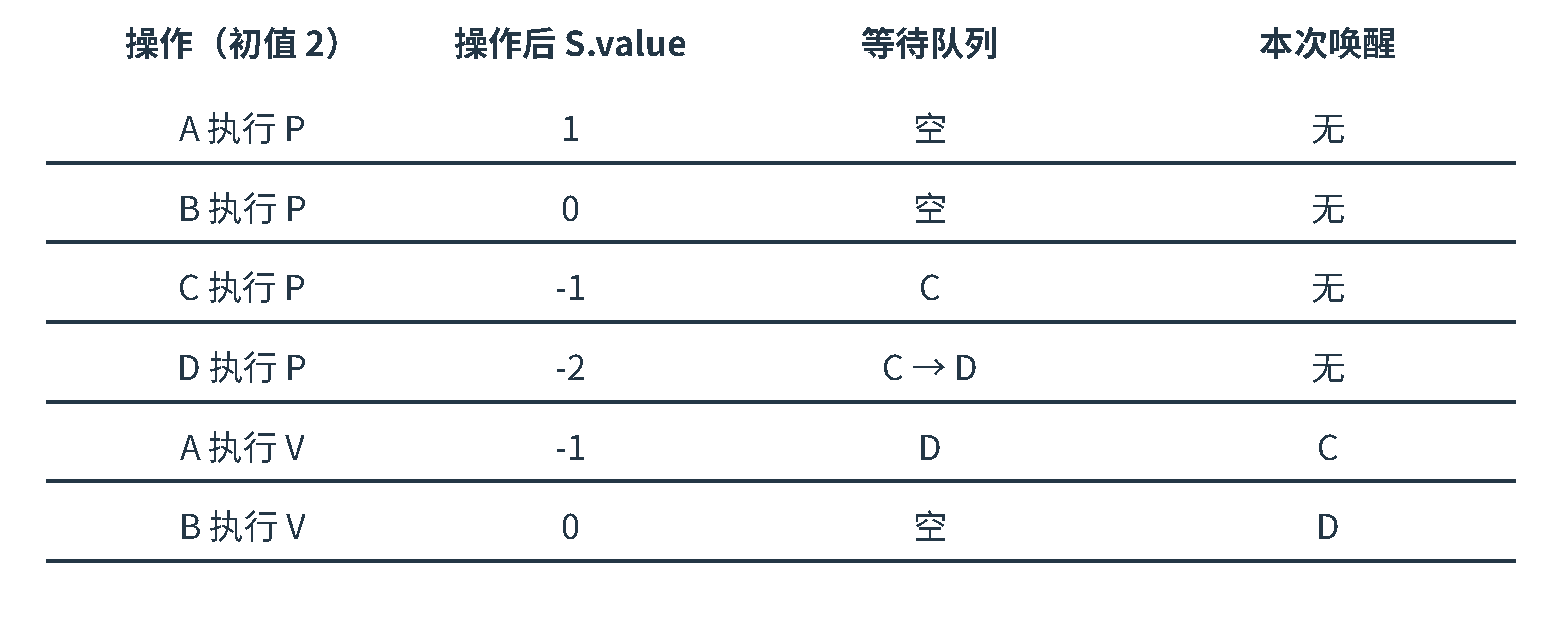
\includegraphics[width=0.95\textwidth,height=\textheight]{figures/F02_signed_semaphore.pdf}
\caption{资源归还会唤醒一个等待者，计数不必先变为正数}\label{fig-signed}
\end{figure}

A 归还后值为 −1，C 已得到可继续执行本次 P 的机会，D 仍等待。此时不能说``值仍是负数，所以 C 还必须再做一次 P''。唤醒 C 也不意味着 C 立即运行；其资源机会与 CPU 调度是两件事。

\subsection{初值来自初态，不来自``同步量''这个名称}\label{os-c03-h133}

互斥量 \texttt{mutex=1} 表示只有一个进入许可。若某项一次性工作尚未完成，完成通知 \texttt{done=0}，后续进程先等通知。若缓冲区已有 \(k\) 个可消费的产品，产品许可应从 \(k\) 开始；容量为 \(n\)、已有 \(k\) 件时，空位许可应为 \(n-k\)。

\subsection{例 3-2　同步信号量一定从 0 开始吗}\label{ex-err18}

\noindent{}〖2.3-018〗 用 P、V 操作实现进程同步，信号量的初值为（　）。

A. −1　　B. 0　　C. 1　　D. 由用户确定

答案为 \textbf{D}。这里的``由用户确定''指根据资源或事件的初始状态确定，不能任意设数。B 适用于尚未发生、尚无可用结果的一次通知，不能覆盖所有同步情形。判断初值时，应检查题目有没有给出``尚未发生''这个限定。

\subsection{将完成条件放在正确位置}\label{os-c03-h145}

若操作 B 必须在 A 完成后开始，设置 \texttt{done=0}：

\par\medskip\noindent
\begin{minipage}{\linewidth}
\begin{verbatim}
前进程：A; V(done);
后进程：P(done); B;
\end{verbatim}
\end{minipage}\par\medskip

若后进程先到，P 使它等待；若前进程先到，V 留下一个许可，后进程后来做 P 时也能通过。通知必须放在 A \textbf{完成之后}，不能在 A 开始前发布。互斥则是各参与者在受保护代码前 P、后 V；同步的一次 P 与产生它的一次 V 通常分布在不同进程中。因此，``P、V 要配合''不等于``必须在同一进程紧挨着出现''。

信号量通常没有互斥锁的持有者限制：一个进程可 P，另一个可 V。这允许它表达合作事件，也意味着不能把信号量与具有所有权要求的 mutex API 完全混同。

\section{从前驱图到线程代码}\label{sec-precedence}

前驱图的边 \(A\to B\) 表示 B 不能在 A 完成前开始。先标出哪些顺序已由同一线程的程序顺序保证，再为剩下的跨线程依赖传递完成通知。给每条边各设一个初值 0 的信号量是常见的直接构造，但已有顺序可能使部分量不再需要；反过来，也不能只因两个操作都等 C，就擅自规定它们互相等待。

\subsection{例 3-3　哪些边需要跨线程通知}\label{ex-2022}

\noindent{}【2022】 某进程的两个线程 T1 和 T2 并发执行 A、B、C、D、E 和 F 共 6 个操作，其中 T1 执行 A、E 和 F，T2 执行 B、C 和 D。题46图表示上述 6 个操作的执行顺序所必须满足的约束：C 在 A 和 B 完成后执行，D 和 E 在 C 完成后执行，F 在 E 完成后执行。请使用信号量的 wait()、signal() 操作描述 T1 和 T2 之间的同步关系，并说明所用信号量的作用及其初值。

\begin{figure}
\centering
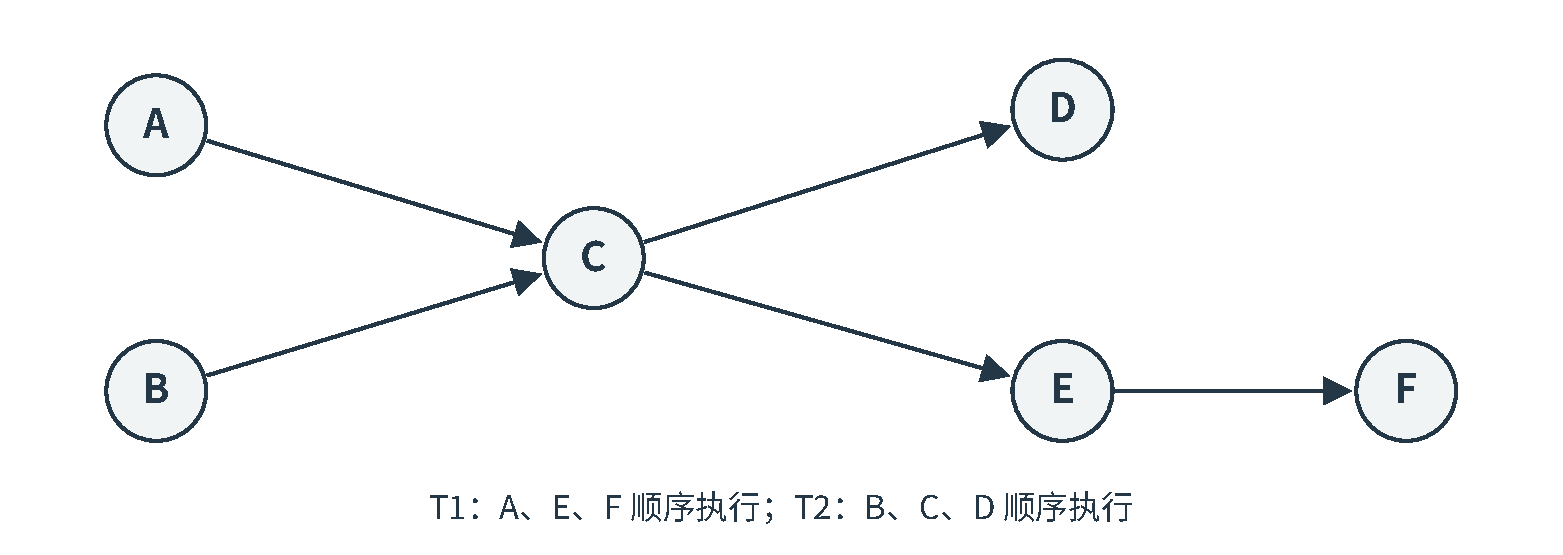
\includegraphics[width=0.96\textwidth,height=\textheight]{figures/F03_precedence_2022.pdf}
\caption{原题前驱图；图下文字标明题干给出的线程归属}\label{fig-precedence}
\end{figure}

\Needspace{6\baselineskip}

\textbf{解析。} 在所写程序中，让 T1 按 A、E、F，T2 按 B、C、D 顺序执行，B→C、C→D、E→F 就已满足。跨线程仍需保证 A→C 和 C→E，分别设 \texttt{S\_AC=0}、\texttt{S\_CE=0}。

\par\medskip\noindent
\begin{minipage}{\linewidth}
\begin{verbatim}
semaphore S_AC = 0, S_CE = 0;

T1() {                 T2() {
    A;                     B;
    signal(S_AC);          wait(S_AC);
    wait(S_CE);            C;
    E;                     signal(S_CE);
    F;                     D;
}                      }
\end{verbatim}
\end{minipage}\par\medskip

T2 到达 C 前已完成本线程的 B，又收到了 A 完成的通知，因此 C 的两个前提齐备。C 完成后先发布 \texttt{S\_CE}，T1 才能开始 E，随后执行 F；T2 自行继续 D。

例如，A、B、C、E、F、D 是允许的完成次序，A、B、C、D、E、F 也允许。D 与 E、F 没有额外次序要求。若把通知放到 D 后，虽然仍不违反图中的先后约束，却会强加 E 等待 D 的限制，减少题目允许的并发。不能把``运行结果安全''误当成``完整保留原约束''。

\section{缓冲区：容量许可与互斥范围分别建立}\label{sec-buffer}

\subsection{例 3-4　同一个缓冲区为什么有不同的信号量方案}\label{ex-2024}

\noindent{}【2024】 计算机系统中的进程之间往往需要相互协作以完成一个任务。在某网络系统中，缓冲区 B 用于存放一个数据分组，对 B 的操作有 C1、C2 和 C3。C1 将一个数据分组写入 B 中，C2 从 B 中读出一个数据分组，C3 对 B 中的数据分组进行修改。要求 B 为空时才能执行 C1，B 非空时才能执行 C2 和 C3。

（1）假设进程 P1 和 P2 均需要执行 C1，实现 C1 的代码是否为临界区？为什么？（2分）

（2）假设 B 初始为空，进程 P1 执行 C1 一次，进程 P2 执行 C2 一次。请定义尽可能少的信号量，并用 wait()、signal() 操作描述进程 P1 和 P2 之间的同步或互斥关系，说明所用信号量的作用及其初值。（3分）

（3）假设 B 初始不为空，进程 P1 和 P2 各执行 C3 一次。请定义尽可能少的信号量，并用 wait()、signal() 操作描述进程 P1 和 P2 之间的同步或互斥关系，说明所用信号量的作用及其初值。（3分）

\Needspace{6\baselineskip}

\textbf{解析。} （1）是。两个 C1 都操作同一缓冲区，若同时发现 B 为空后分别写入，可能覆盖数据；检查并改变缓冲状态的代码需要保护。

（2）先把``初始为空、各一次''转成 C1 完成→C2 开始。设置 \texttt{done=0}，表示唯一一次写入完成的通知：

\par\medskip\noindent
\begin{minipage}{\linewidth}
\begin{verbatim}
semaphore done = 0;
P1() { C1; signal(done); }
P2() { wait(done); C2; }
\end{verbatim}
\end{minipage}\par\medskip

零个同步量不能阻止 P2 先读；一个量已经使 C2 必在 C1 之后，两次操作不会重叠，故无需再加互斥量。这里是同步关系已经保证本情境下的互斥，不能据\hyperref[ex-err11]{例3-1}的分类机械增加变量。

（3）B 已非空，且这里只有两个 C3，修改不会将 B 清空。无需等待新的产品，只须保证两次修改不重叠：

\par\medskip\noindent
\begin{minipage}{\linewidth}
\begin{verbatim}
semaphore mutex = 1;
P1() { wait(mutex); C3; signal(mutex); }
P2() { wait(mutex); C3; signal(mutex); }
\end{verbatim}
\end{minipage}\par\medskip

三问的共享对象相同，操作类型与执行次数却不同。``容量为 1''不能单独决定信号量个数；必须把参与者、初态和活动范围一起代入。

\subsection{有限缓冲区为什么通常需要 empty、full 和 mutex}\label{os-c03-h220}

经典生产者---消费者模型中，一组生产者反复放入，一组消费者反复取走，共享容量为 \(n>0\)、初始为空的缓冲区。每次放入或取出一件，操作缓冲区及其相关指针需要互斥。基本模型见王道书 §2.3。

三项条件分别决定三种许可：\texttt{empty=n} 表示尚未被申请的空槽，\texttt{full=0} 表示尚未被申请的产品，\texttt{mutex=1} 保护单次缓冲操作。生产者在本地生产、消费者在本地使用产品，均无需占用缓冲区锁。

\begin{figure}
\centering
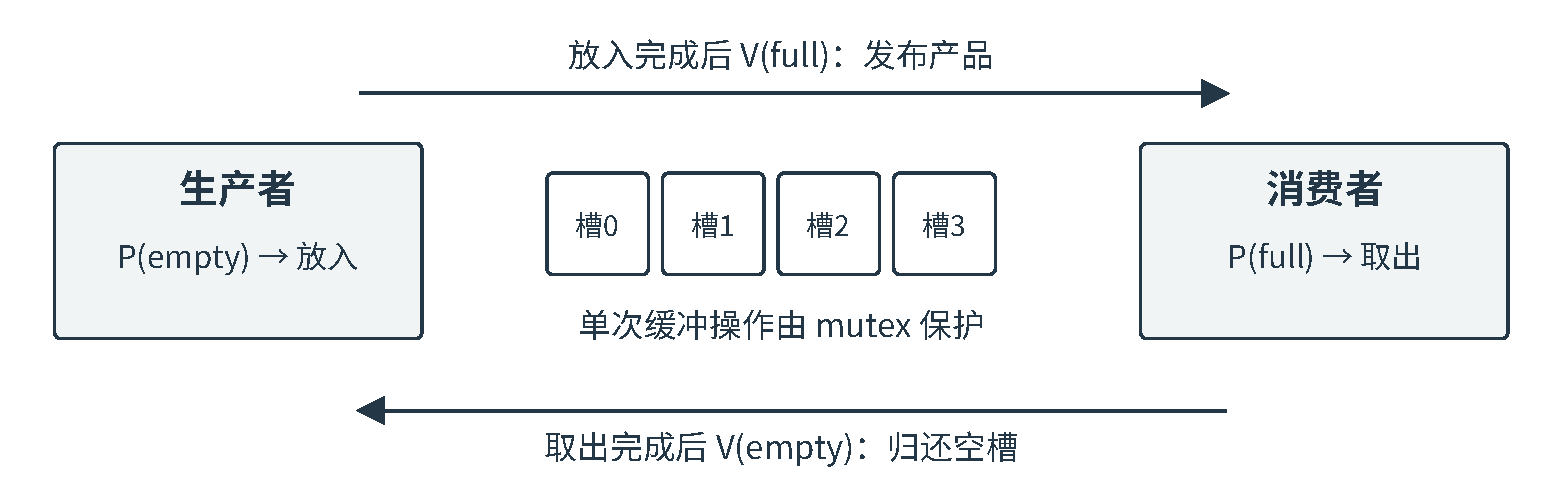
\includegraphics[width=0.96\textwidth,height=\textheight]{figures/F04_buffer_permissions.pdf}
\caption{空位许可与产品许可沿相反方向流动；四个槽只是示意，算法容量仍为 n}\label{fig-buffer}
\end{figure}

\par\medskip\noindent
\begin{minipage}{\linewidth}
\begin{verbatim}
semaphore empty = n, full = 0, mutex = 1;

producer() {
    while (true) {
        x = produce();
        P(empty);          // 先取得一个空槽许可
        P(mutex);
        put(x);
        V(mutex);
        V(full);           // 放入完成，才能发布产品
    }
}
\end{verbatim}
\end{minipage}\par\medskip

\par\medskip\noindent
\begin{minipage}{\linewidth}
\begin{verbatim}
consumer() {
    while (true) {
        P(full);           // 先取得一个产品许可
        P(mutex);
        x = get();
        V(mutex);
        V(empty);
        consume(x);
    }
}
\end{verbatim}
\end{minipage}\par\medskip

``尚未被申请''不能省略。容量为 2、初始为空时，一个生产者刚执行 P(empty) 而尚未放入，\texttt{empty=1,}\allowbreak{}\texttt{\ full=0}，物理空槽却仍有 2 个。空槽已预留，信号量先减少，实际空位数还没变；消费者取得 \texttt{full} 后、实际取出前也类似。因此不能把执行中每一步的 \texttt{empty+full} 都写成 \(n\)，也不能把 \texttt{full} 无条件等同于实存产品数。两个计数均非负，且既无已取得但尚未使用的许可，也无操作完成却尚未发布的许可时，才可把它们分别与物理空槽数、产品数对照。计数为负时，其绝对值表示相应等待者数。

\subsection{为什么不能持有缓冲区锁等待产品}\label{os-c03-h258}

若消费者先 \texttt{P(mutex)} 再 \texttt{P(full)}，初始为空时，它会持锁阻塞。生产者随后申请 \texttt{mutex} 也阻塞；消费者等生产者放入，生产者等消费者解锁，形成等待环。

\begin{figure}
\centering
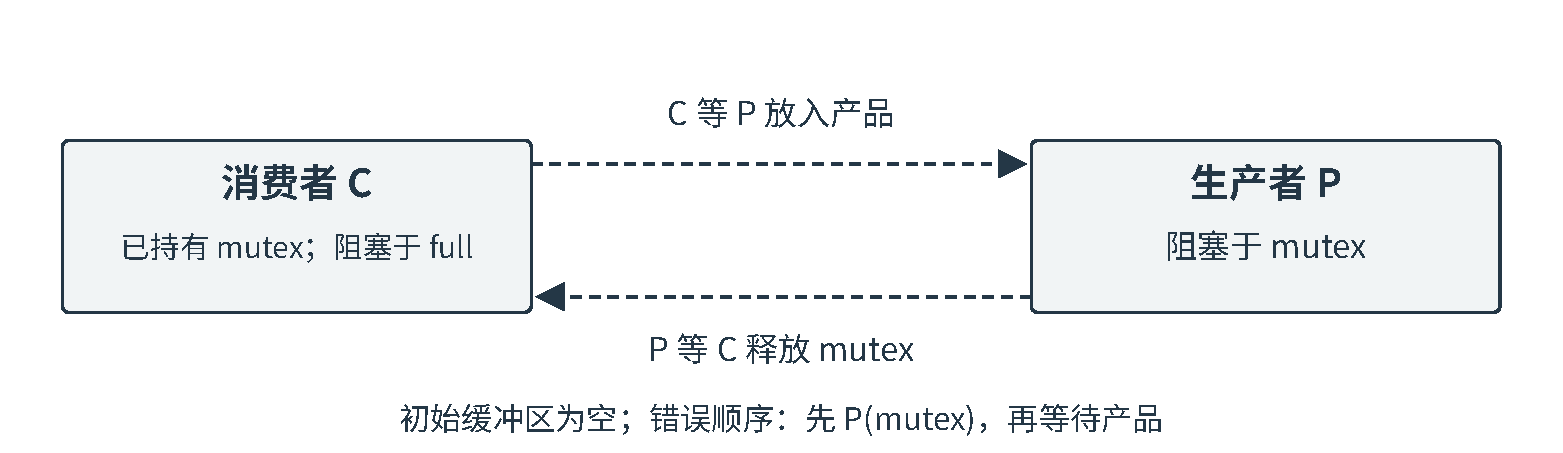
\includegraphics[width=0.96\textwidth,height=\textheight]{figures/F05_buffer_deadlock.pdf}
\caption{错误的 P 顺序使能够改变条件的进程也被挡住}\label{fig-deadlock}
\end{figure}

所以在这个算法中，容量或产品的 P 在外，缓冲区锁的 P 在内。判断别的算法时仍要追问：当前持有什么，等待什么，谁能使条件成立，对方是否也要用所持资源。不能把``同步 P 总在所有互斥 P 前''背成普遍定理；\hyperref[ex-2014]{整批取数}和\hyperref[sec-readers]{读者组}会给出更具体的锁范围。

放入之后，本算法的 \texttt{V(mutex)} 与 \texttt{V(full)} 可交换：消费者即使先收到产品许可，仍须取得 \texttt{mutex} 才能取出。原顺序可避免提前唤醒后再等锁。这个判断依赖放入已经完成、且后续访问也持锁；不是所有 V 都能任意挪动。

\noindent{}〖2.3-039〗 生产者---消费者模型处理的是进程之间的同步与互斥。它不自动保证公平；错误的 P 顺序还可能制造死锁。避免这一错误顺序，是正确实现的条件，不能据此声称该模型能解决任意死锁。

\subsection{例 3-5　消费者只能取特定类别时怎样计数}\label{ex-2009}

\noindent{}【2009】 三个进程 P1、P2、P3 互斥使用一个包含 N（N\textgreater0）个单元的缓冲区。P1 每次用 produce() 生成一个正整数并用 put() 送入缓冲区某一空单元中；P2 每次用 getodd() 从该缓冲区中取出一个奇数并用 countodd() 统计奇数个数；P3 每次用 geteven() 从该缓冲区中取出一个偶数并用 counteven() 统计偶数个数。请用信号量机制实现这三个进程的同步与互斥活动，并说明所定义信号量的含义（要求用伪代码描述）。

\Needspace{6\baselineskip}

\textbf{解析。} ``缓冲区非空''不足以允许 P2 取数：其中可能只有偶数。保留共同的空位许可，把产品许可按可取条件拆为 \texttt{odd} 与 \texttt{even}；三种缓冲操作共用 \texttt{mutex}。

原题未明说缓冲区初态。以下按参考答案采用\textbf{初始为空}：\texttt{empty=N,}\allowbreak{}\texttt{\ odd=even=0,}\allowbreak{}\texttt{\ mutex=1}。令 \texttt{x} 是 P1 本次生成的本地整数，\texttt{put()} 放入它；保留题设函数名。

\par\medskip\noindent
\begin{minipage}{\linewidth}
\begin{verbatim}
semaphore empty = N, odd = 0, even = 0, mutex = 1;

P1() {
    while (true) {
        x = produce();
        P(empty);
        P(mutex);
        put();
        V(mutex);
        if (x % 2 != 0) V(odd); else V(even);
    }
}
\end{verbatim}
\end{minipage}\par\medskip

\par\medskip\noindent
\begin{minipage}{\linewidth}
\begin{verbatim}
P2() {
    while (true) {
        P(odd);
        P(mutex);
        getodd();
        V(mutex);
        V(empty);
        countodd();
    }
}
\end{verbatim}
\end{minipage}\par\medskip

\par\medskip\noindent
\begin{minipage}{\linewidth}
\begin{verbatim}
P3() {
    while (true) {
        P(even);
        P(mutex);
        geteven();
        V(mutex);
        V(empty);
        counteven();
    }
}
\end{verbatim}
\end{minipage}\par\medskip

每次 put 只发布其所属类别的一份许可，消费者不能拿另一类别的许可代用。getodd/geteven 完成后，空位可立刻交还；各自的统计不访问共享缓冲区，留在锁外。

若初始已有 \(a\) 个奇数、\(b\) 个偶数，则应改为 \texttt{odd=a,}\allowbreak{}\texttt{\ even=b,}\allowbreak{}\texttt{\ empty=N-a-b}，其中 \(a,b\ge0\) 且 \(a+b\le N\)。若输入长期没有某类别，该类别消费者可以持续等待；只要生产者和另一消费者仍前进，就不能仅凭这一等待认定系统死锁。题目没有保证所有类别都会出现。

\subsection{例 3-6　连续取 10 件改变的是哪一层互斥}\label{ex-2014}

\noindent{}【2014】 系统中有多个生产者进程和多个消费者进程，共享一个能存放 1000 件产品的环形缓冲区（初始为空）。当缓冲区未满时，生产者进程可以放入其生产的一件产品，否则等待；当缓冲区未空时，消费者进程可以从缓冲区取走一件产品，否则等待。要求一个消费者进程从缓冲区连续取出 10 件产品后，其他消费者进程才可以取产品。请使用信号量 P、V（或 wait()、signal()）操作实现进程间的互斥与同步，要求写出完整的过程，并说明所用信号量的含义和初值。

\Needspace{6\baselineskip}

\textbf{解析。} ``连续''限制其他消费者插入取数，不禁止生产者在这期间补货。由此需要两个范围：\texttt{mutex=1} 保护一次缓冲操作，\texttt{batch=1} 由一个消费者持有直到它取满 10 件。生产者不申请 \texttt{batch}。

\par\medskip\noindent
\begin{minipage}{\linewidth}
\begin{verbatim}
semaphore empty = 1000, full = 0, mutex = 1, batch = 1;
item buf[1000];
int in = 0, out = 0;

producer() {
    while (true) {
        x = produce();
        P(empty);
        P(mutex);
        buf[in] = x;
        in = (in + 1) % 1000;
        V(mutex);
        V(full);
    }
}
\end{verbatim}
\end{minipage}\par\medskip

\par\medskip\noindent
\begin{minipage}{\linewidth}
\begin{verbatim}
consumer() {
    while (true) {
        P(batch);
        for (int k = 0; k < 10; ++k) {
            P(full);
            P(mutex);
            local[k] = buf[out];
            out = (out + 1) % 1000;
            V(mutex);
            V(empty);
        }
        V(batch);
        consume(local);
    }
}
\end{verbatim}
\end{minipage}\par\medskip

\texttt{empty}、\texttt{full} 的含义与初值来自容量和初态。\texttt{in/out} 分别指向下一次放入、取出的位置；\texttt{local{[}0..9{]}} 是消费者私有的十件产品存储。每次取走一件就归还一个空槽，不必等整批结束。

假设消费者已取出 3 件，缓冲区暂时为空。它持有 \texttt{batch}，等 \texttt{full}；但它没有持有 \texttt{mutex}，生产者能继续放入并 V(full)，因此可接着取第 4 件。其他消费者不能插入，所要求的连续性得到保持。若把 \texttt{mutex} 从整批开头一直持有到末尾，消费者会在缺货时挡住补货者，形成死锁。

本解不要求开始时凑齐 10 件。不要让多个消费者在批锁之外各申请若干产品许可，再等凑够十个；这会把产品预留给多个消费者，破坏整批协调。\texttt{batch} 在前并非违反上一节的锁顺序：真正要检查的是生产者是否也依赖它，以及消费者等待产品时是否仍给生产者留下执行通路。

\section{多个读者怎样作为一组申请资源}\label{sec-readers}

读者---写者模型允许多个读者同时读共享文件；写者之间互斥，写者与任何读者互斥。读者读完不清空文件，因此``已有数据''不应被当作一个被读走就消耗的产品许可。以下采用王道书 §2.3 的经典模型；一次读或写有限，所有访问者遵守同一协议。

\subsection{首读者申请，末读者释放}\label{os-c03-h375}

令 \texttt{rw=1} 表示文件访问权：一个写者独占，或者一组读者共同持有。共享计数 \texttt{readCount=0} 记录已登记但尚未退出的读者数，\texttt{countMutex=1} 保护该计数和首末读者判断。

\par\medskip\noindent
\begin{minipage}{\linewidth}
\begin{verbatim}
semaphore rw = 1, countMutex = 1;
int readCount = 0;

reader() {
    P(countMutex);
    if (readCount == 0) P(rw);
    readCount++;
    V(countMutex);

    读文件;

    P(countMutex);
    readCount--;
    if (readCount == 0) V(rw);
    V(countMutex);
}
\end{verbatim}
\end{minipage}\par\medskip

\par\medskip\noindent
\begin{minipage}{\linewidth}
\begin{verbatim}
writer() {
    P(rw);
    写文件;
    V(rw);
}
\end{verbatim}
\end{minipage}\par\medskip

第一个读者为整组取得 \texttt{rw}，后续读者只登记，不重复申请 \texttt{rw}；最后一个读者离开才归还。若每个读者都在读文件前 P(rw)、读后 V(rw)，读者也被串行化，题目允许的并发便丢失了。

\begin{figure}
\centering
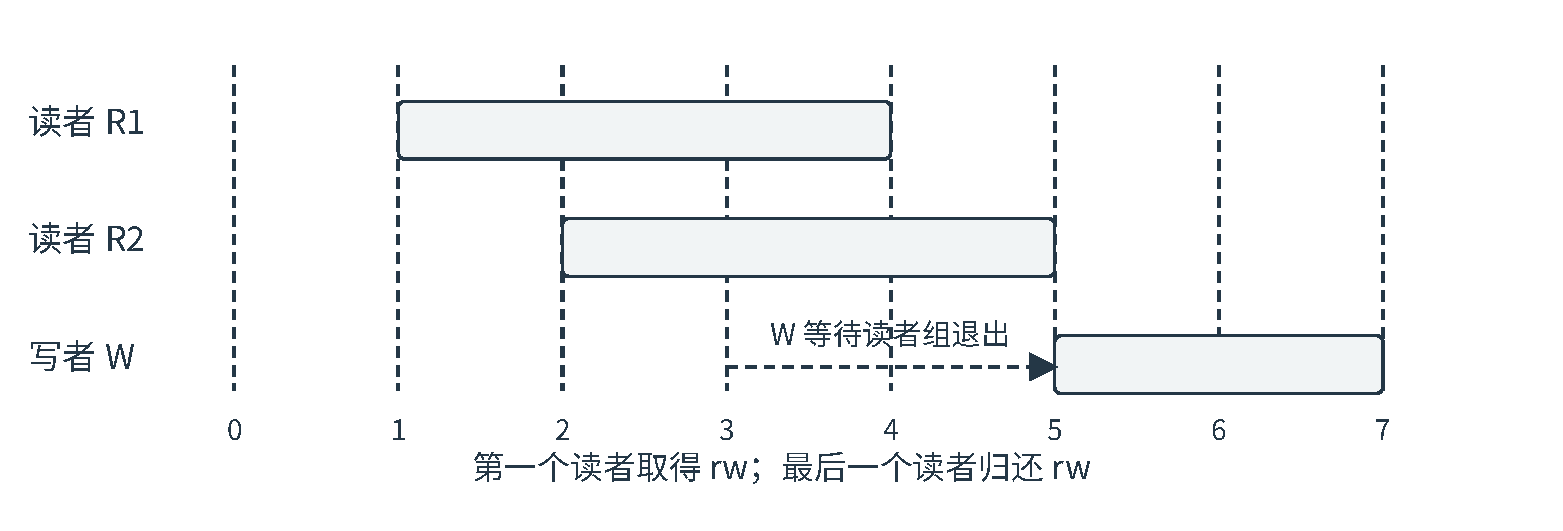
\includegraphics[width=0.96\textwidth,height=\textheight]{figures/F06_readers_group.pdf}
\caption{重叠的两个读者共同占有一个读者组的文件访问权；横轴为示意时间}\label{fig-readers}
\end{figure}

计数的检查和修改须在同一个受保护范围。假设只保护加减、不保护前面的判断：\texttt{readCount=1} 时，新读者检查到非零，准备跳过 P(rw)，此时暂停；原有的最后一个读者退出，把计数减到 0 并释放 rw；写者取得 rw 后，新读者才恢复，将计数加 1 并开始读。新读者没有申请 rw，却与写者同时访问。把判断和登记一起保护，才能排除这条交错。

首读者可能持有 \texttt{countMutex} 等待 \texttt{rw}，此处为何不必然死锁？它等待时 \texttt{readCount=0}，所以没有已登记的读者需要取得 \texttt{countMutex} 来做末读者退出；正在写的进程归还 \texttt{rw} 也不需要 \texttt{countMutex}。

\subsection{读者优先与公平需要分别说明}\label{os-c03-h414}

上述算法中，只要仍有读者在读，新来的读者就能加入同一组，即使已有写者等 \texttt{rw}。不断到来的读者可能使 \texttt{readCount} 始终不归零，写者因而饥饿。

一种改法是加入口信号量 \texttt{gate=1}。每个读者在登记前 P(gate)，登记后 V(gate)；写者则 P(gate)、P(rw)，写完后依次 V(rw)、V(gate)。其余读者退出代码不变：

\par\medskip\noindent
\begin{minipage}{\linewidth}
\begin{verbatim}
// 读者的入口，替换上一算法的入口部分
P(gate);
P(countMutex);
if (readCount == 0) P(rw);
readCount++;
V(countMutex);
V(gate);

// 写者完整过程
P(gate);
P(rw);
写文件;
V(rw);
V(gate);
\end{verbatim}
\end{minipage}\par\medskip

一旦写者取得 \texttt{gate}，新读者不能再登记；原有读者仍能按原退出代码离开，最后一个释放 \texttt{rw}，写者便可进入。若 \texttt{gate} 队列按先进先出服务，且进程持续获得执行机会、读写有限，可进一步说明等待者不会被后来者无限越过。\textbf{仅有信号量而没有公平排队约定，不能无条件宣称``不会饥饿''或``严格先来先服务''。} 这也不是无论到达次序如何都让写者先于读者的绝对写优先策略。

\section{哲学家进餐：申请多个资源时怎样断开等待环}\label{sec-philosophers}

五个哲学家 \(P_0\) 至 \(P_4\) 围桌而坐，每人须同时持有左右两根筷子才能吃饭。一根筷子只供一人使用，吃完归还，再思考。统一编号：\(P_i\) 需要 \(C_i\) 与 \(C_{(i+1)\bmod5}\)，每个筷子量初值为 1。经典模型见王道书 §2.3。

如果所有人都先 P(C{[}i{]}) 再 P(C{[}(i+1)\%5{]})，一种允许的交错是每人先拿到一根。此时所有人等右邻已持有的另一根，无人能到达归还步骤。

\begin{figure}
\centering
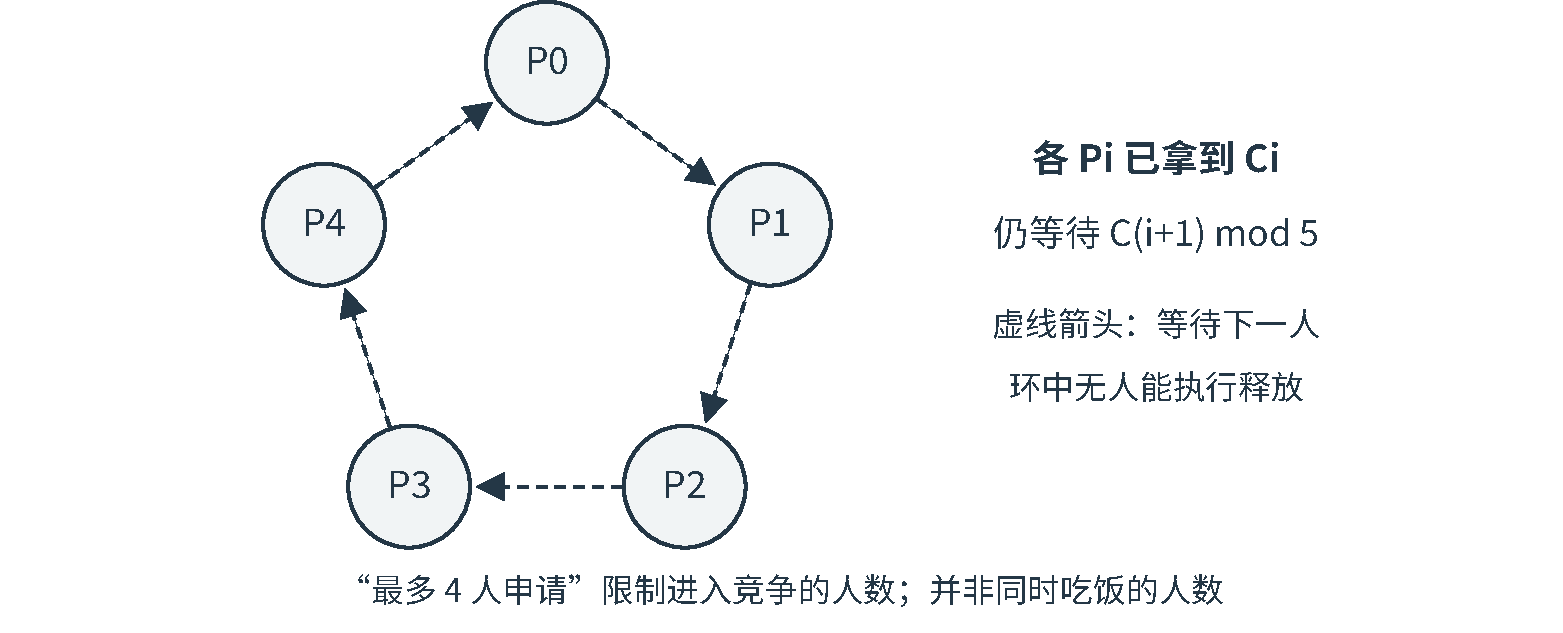
\includegraphics[width=0.96\textwidth,height=\textheight]{figures/F07_philosopher_wait_cycle.pdf}
\caption{每个进程只持有一根筷子，也足以形成整体死锁}\label{fig-philosophers}
\end{figure}

\subsection{限制竞争人数，与限制同时吃饭人数不同}\label{os-c03-h447}

增加 \texttt{room=4}，使最多四人处在``开始拿筷子到全部归还''的区间内：

\par\medskip\noindent
\begin{minipage}{\linewidth}
\begin{verbatim}
semaphore room = 4;
semaphore C[5] = {1, 1, 1, 1, 1};

philosopher(i) {
    while (true) {
        思考;
        P(room);
        P(C[i]);
        P(C[(i+1) % 5]);
        吃饭;
        V(C[(i+1) % 5]);
        V(C[i]);
        V(room);
    }
}
\end{verbatim}
\end{minipage}\par\medskip

若所有竞争者都各持一根并等待下一根，要形成完整环就必须五人都参与；\texttt{room=4} 阻止了这种状态。沿等待方向追下去，会遇到未占筷子的缺口或正在吃饭、能够归还筷子的人。只要持有者继续执行、进餐有限，就不会陷入上述整体等待环。

这里的 4 是同时申请区间内的人数上限。五根筷子最多支持 \(\lfloor5/2\rfloor=2\) 人同时吃饭，不能把``最多四人申请''误读为``四人同时进餐''。该办法排除了这个死锁模型，不自动保证某一饥饿者最终抢到许可；仍需公平条件。

另一种办法是全局排序：所有人都先取编号较小、再取较大的筷子。若存在资源等待环，沿环等待的资源编号就必须严格递增，最后又回到起点，不可能成立。每人独立``先左后右''不是全局排序；编号相邻位置在取模后更须检查。

也可用额外互斥量把``拿两根''的过程串行化，拿齐后立即释放这个额外量，吃完直接归还筷子。这能断开多人各拿一根的环，但可能让一个正在等筷子的人挡住另一个本可拿齐的人。它也不等于``先原子检查两根都空闲，然后同时取得''；若题目要求整组资源同时分配，就需要更强的原子检查与分配机制。

\section{管程与条件变量：等待时必须让出改变条件的机会}\label{sec-monitor}

\textbf{管程}把共享数据、对数据的操作过程和初始化封装在一个同步模块中，参与者通过规定入口访问共享数据；同一时刻至多一个进程在其中执行。这个互斥规则由实现管程的语言或运行系统保证，不要求调用者在每个入口外重复编写 P、V。管程不是一个自行运行的进程。

但``每次只准一人进入''还不够：消费者进入后可能发现无产品。若它在管程里循环等待并一直保有管程，生产者就无法进入改变条件。\textbf{条件变量}为这种等待提供队列；实际条件由共享数据上的布尔判断表达，例如 \texttt{count\textgreater{}0}。条件变量本身不是保存产品数的整数。

\subsection{wait 负责等待，不替调用者判断条件}\label{os-c03-h483}

\subsection{例 3-7　条件变量的 wait 做什么}\label{ex-2018}

\noindent{}【2018】 若 x 是管程内的条件变量，则当进程执行 x.wait() 时所做的工作是（　）。

A. 实现对变量 x 的互斥访问

B. 唤醒一个在 x 上阻塞的进程

C. 根据 x 的值判断该进程是否进入阻塞态

D. 阻塞该进程，并将之插入 x 的阻塞队列中

答案为 \textbf{D}。调用者先检查共享状态，只有需要等待时才调用 x.wait()；调用后进入 x 的等待队列，并释放管程使用权，让其他进程能进入。C 把``调用前的条件判断''放进了 wait 的职责，还把 x 当作可直接判值的资源计数。

管程中执行 x.signal()，是通知一个已经在 x 上等待的进程。若没有等待者，通知不积累；以后进入的进程须重新检查共享状态。信号量 V 即使没有等待者，也会使计数增加，留下一个可供后续 P 使用的许可。

\noindent{}〖2.3-029〗 ``管程中 signal 操作的作用和信号量机制中的 V 操作相同''不成立。检查无等待者的边界即可区分：前者不留下通知，后者增加许可。管程作为同步模块，与一个可独立运行的进程也不是同一类对象；具体语言的管程对象能否实例化，应由语言规定。

\subsection{通知以后，何时重新检查条件}\label{os-c03-h503}

不同管程定义对 signal 后的运行次序有不同规定。Hoare 式语义可立即转交管程给被唤醒者；Mesa 式语义让通知者继续，等待者以后重新竞争进入权。题目若给出特定语义，应据此推演，不能混用。

下面用 Mesa / POSIX 式条件等待说明可独立执行的做法。\texttt{wait(cv,}\allowbreak{}\texttt{m)} 把``释放互斥锁 m 与进入等待''衔接为原子等待操作；返回前重新取得 m。通知不保证等待者马上运行，也不保证等它重新取得 m 时条件仍成立，所以用 \texttt{while} 重检。实际接口还可能出现虚假唤醒，同样需要重检。

\begin{figure}
\centering
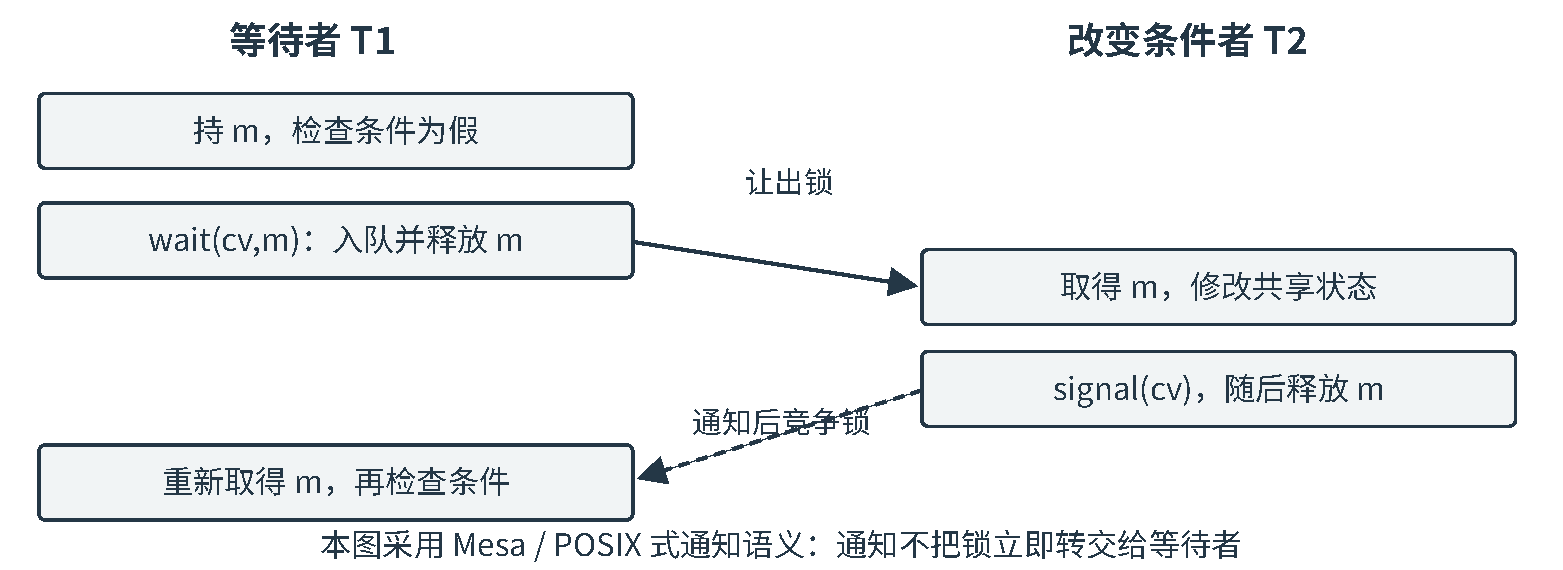
\includegraphics[width=0.96\textwidth,height=\textheight]{figures/F08_condition_wait.pdf}
\caption{wait 释放锁，使另一个线程能够改变共享状态；等待返回前须重新取得锁}\label{fig-monitor}
\end{figure}

设这个模块的容量为 \(n>0\)，初始为空，m 初始化为未加锁；插入和取出维护同一个缓冲区。

\par\medskip\noindent
\begin{minipage}{\linewidth}
\begin{verbatim}
// 单个缓冲模块的共享状态
mutex m;
condition notEmpty, notFull;
int count = 0;

put(x) {
    lock(m);
    while (count == n) wait(notFull, m);
    插入 x; count++;
    signal(notEmpty);
    unlock(m);
}
\end{verbatim}
\end{minipage}\par\medskip

\par\medskip\noindent
\begin{minipage}{\linewidth}
\begin{verbatim}
get() {
    lock(m);
    while (count == 0) wait(notEmpty, m);
    x = 取出元素; count--;
    signal(notFull);
    unlock(m);
    return x;
}
\end{verbatim}
\end{minipage}\par\medskip

若消费者发现空就调用 wait，它释放 m；生产者才能取得 m 放入，并通知消费者。被通知者回来时再次检查 \texttt{count}，是因为这期间可能已有另一个消费者先取走产品。不能把 \texttt{wait} 拆成普通的``先 unlock，再单独入队''：另一线程可能恰在两步之间发出无人接收的通知，等待者随后入队，就错过了这次机会。

这里的接口语义用于把等待机制讲清，并非要求记忆 POSIX 参数及错误码。参见 The Open Group《Base Specifications Issue 8》条件等待与通知条目；管程概念与条件变量的比较见王道书 §2.3。

\section{写出并发代码后，怎样检验}\label{sec-method}

题干中的名词不会直接决定信号量个数。先把每个进程的一次活动写清，标出它开始前必须成立的条件，再说明谁能使该条件成立。把``可用槽位''``某类产品''``阶段已经完成''等条件转成许可，把会冲突的共享状态操作放进相应互斥范围，才能确定变量及初值。

\begin{longtable}[]{@{}
  >{\raggedright\arraybackslash}p{(\columnwidth - 4\tabcolsep) * \real{0.2942}}
  >{\raggedright\arraybackslash}p{(\columnwidth - 4\tabcolsep) * \real{0.3256}}
  >{\raggedright\arraybackslash}p{(\columnwidth - 4\tabcolsep) * \real{0.3801}}@{}}
\toprule\noalign{}
\begin{minipage}[b]{\linewidth}\raggedright
题干给出的条件
\end{minipage} & \begin{minipage}[b]{\linewidth}\raggedright
转成什么关系
\end{minipage} & \begin{minipage}[b]{\linewidth}\raggedright
应检查的代码位置
\end{minipage} \\
\midrule\noalign{}
\endhead
\bottomrule\noalign{}
\endlastfoot
必须等某操作完成 & 完成通知，初值由该事件是否已发生决定 & 前操作完成后 V，后操作开始前 P。 \\
最多容纳 n 件 & 容量许可，有放入与归还两个方向 & 先申请空位，放入后发布产品，取出后归还空位。 \\
只能取某一类 & 每一类独立的可取条件 & 发布对应类别，不用总 full 冒充所有消费者的许可。 \\
多个读者可以并行 & 读者组与写者互斥 & 保护首末读者判断，而非将整个读操作串行化。 \\
连续取 k 件后才轮到别人 & 消费者整批排他 & 批锁覆盖 k 次，缓冲锁只覆盖单次；等待时允许补货。 \\
\end{longtable}

最后手推几条会暴露错误的轨迹：后继先运行、缓冲区初始为空或已满、两个请求几乎同时到达、一个进程拿到许可但尚未实际操作、通知发出但被通知者尚未重新运行。每一步记下``持有---等待---可执行者''。检查安全性后，再分别检查死锁、饥饿与不必要的串行化；三者不能互相代替。

\section{自测：先判断，再看答案}\label{sec-selfcheck}

原创回顾设问：下列问题依据本章例题与经典模型编写，用于检查中间状态和适用边界。

\begin{enumerate}
\def\labelenumi{\arabic{enumi}.}
\tightlist
\item
  按\hyperref[sec-semaphore]{记录型语义}，P 前 \texttt{S.value=1}，P 后为 0，要阻塞吗？一次 V 使值从 −1 变为 0，要唤醒吗？被唤醒者是否还要为这次申请再减 1？
\item
  在\hyperref[ex-2022]{2022 年前驱题}中，能否在 D 完成后才 signal(S\_CE)？这样是否保留了图允许的所有并发？
\item
  在\hyperref[ex-2009]{分类缓冲题}中，初态有 \(a\) 个奇数、\(b\) 个偶数，三个计数量怎样初始化？如果缓冲区只有偶数，P2 等待能否说明整个系统死锁？
\item
  在\hyperref[ex-2014]{成批取数题}中，某消费者取了 3 件后暂时缺货，应继续持有哪个量、等待哪个量？生产者还能否运行？
\item
  哲学家最多允许四人进入申请区，是否能有四人同时吃饭？
\item
  条件变量 signal 在没有等待者时，是否留下一份以后可取得的许可？
\end{enumerate}

\subsection{自测答案}\label{os-c03-h568}

\begin{enumerate}
\def\labelenumi{\arabic{enumi}.}
\tightlist
\item
  P 后为 0 不阻塞，表示取走最后一个许可。V 后为 0 仍须唤醒一个等待者；它已取得本次申请的机会，不再为同一次 P 减 1。
\item
  能保证 E 不早于 C，却额外让 E 等 D，缩小并发范围。通知应在 C 完成后、D 前发出。
\item
  \texttt{empty=N-a-b,}\allowbreak{}\texttt{\ odd=a,}\allowbreak{}\texttt{\ even=b}；需 \(a,b\ge0\)、\(a+b\le N\)。只有 P2 无奇数可取，不能推出整个系统无法前进。
\item
  持有 \texttt{batch}、等待 \texttt{full}，此时没有持有 \texttt{mutex}。生产者不需要 \texttt{batch}，仍能取得空位与缓冲区锁，补入产品。
\item
  最多两人同时吃饭，四是申请区间内的人数上限。
\item
  条件变量通知不积累为以后可消费的许可；有资源初态要用共享状态表达。
\end{enumerate}

条件变量等待语义另参 The Open Group 条件等待与通知接口、Oracle《Using Condition Variables》。

\chapter{死锁：从资源分配状态判断能否继续}\label{os-ch4}

进程因为没有资源而等待，并不一定发生死锁。必须继续追问：谁持有它所需的资源，持有者能否完成并归还，归还又依赖谁。本章把这种追踪分别用于死锁条件、资源分配图、安全检查和死锁检测。

除特别说明，讨论的是可重复使用的资源：每类可以有多个同类实例，资源只能在释放后再次分配；进程请求后若不能满足便等待，正常完成会归还已持资源。分析安全性还假定进程声明的最大需求可信，不超过系统允许的资源总量，并能在获得所需资源后有限完成。

\section{死锁、饥饿和不安全状态}\label{os-4-1}

\textbf{死锁}指一组进程中，每个进程都在等待只能由组内进程引起的事件（也可能是自身尚未执行的释放动作），因而这一组无法自行推进。最小的双资源例子是：P 持有 A 等 B，Q 持有 B 等 A；没有进程能到达释放步骤。

\textbf{饥饿}指某个进程长期得不到所需服务，而其他进程仍可能持续前进。例如读者不断加入，使写者一直拿不到写权限。\textbf{死循环}是执行路径自身不能结束，进程可能仍持续占用 CPU，不必等待其他进程。三者的机制不同，处理方法也不同。

\subsection{四个必要条件是同时约束}\label{os-c04-h13}

\begin{longtable}[]{@{}
  >{\raggedright\arraybackslash}p{(\columnwidth - 4\tabcolsep) * \real{0.2573}}
  >{\raggedright\arraybackslash}p{(\columnwidth - 4\tabcolsep) * \real{0.3783}}
  >{\raggedright\arraybackslash}p{(\columnwidth - 4\tabcolsep) * \real{0.3643}}@{}}
\toprule\noalign{}
\begin{minipage}[b]{\linewidth}\raggedright
条件
\end{minipage} & \begin{minipage}[b]{\linewidth}\raggedright
本章资源模型中的含义
\end{minipage} & \begin{minipage}[b]{\linewidth}\raggedright
怎样在状态中识别
\end{minipage} \\
\midrule\noalign{}
\endhead
\bottomrule\noalign{}
\endlastfoot
互斥 & 某类实例同一时刻只能给一个进程使用 & 资源不可被两个申请者同时使用 \\
占有并等待 & 保持已有资源，同时等待新增资源 & 一个进程既有分配边，又有请求边 \\
不可剥夺 & 未用完的资源不能被系统任意收回 & 只能由持有者按规则释放 \\
循环等待 & 存在首尾相接的资源等待链 & P 等 Q，Q 又直接或间接等 P \\
\end{longtable}

发生这类资源死锁时，四项同时成立；只满足其中一项或几项不能推出死锁。``四项必要条件都允许存在''也不等于任何时刻都已经死锁，还要检查实际持有与等待状态。单进程再次请求一个自己已经持有且不可重入的锁，也可能自我阻塞，不能把``死锁至少要两个进程''当作适用于所有锁语义的结论。

\subsection{资源分配图中的环什么时候足够}\label{os-c04-h24}

进程用圆表示，资源类型用方框表示，框内点表示实例。\(P_i\to R_j\) 是请求边，\(R_j\to P_i\) 是一个实例的分配边。没有有向环，可排除这种资源等待死锁；有环时，若环中相关资源类型均只有一个实例，则可判定死锁。

若资源类型有多个实例，环只说明可能死锁。例如 P 持有 A 的一个实例、等待 B，Q 持有 B、等待 A，但 A 还有一个空闲实例，Q 取得它并完成后就能释放 B。图中已有等待环，却仍有解开它的执行通路。此时必须结合实例数化简或执行检测算法。

\begin{figure}
\centering
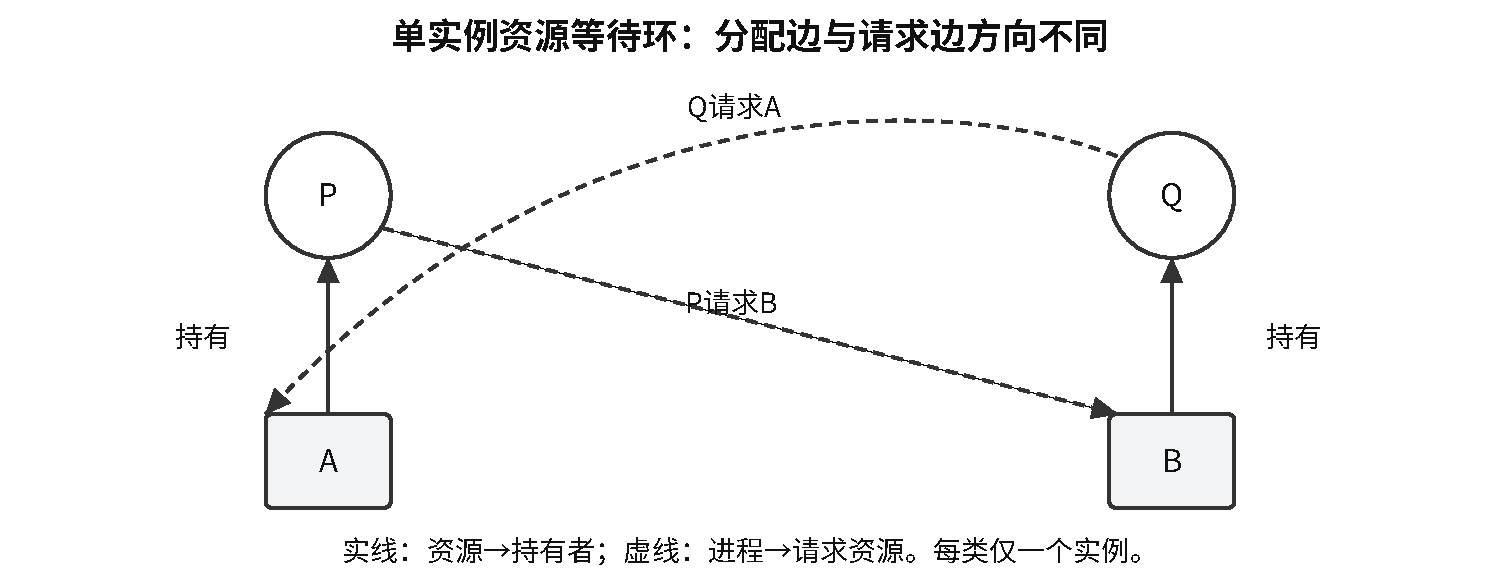
\includegraphics[width=0.95\textwidth,height=\textheight]{figures/OS_resource_graph.pdf}
\caption{单实例环中每个人都等别人；增加可用实例后必须重新检查能否推进}\label{os-fig-resource}
\end{figure}

\subsection{安全状态问的是``能否保证全部完成''}\label{os-c04-h32}

\textbf{安全序列}是进程的一种次序，使每个进程在轮到它时，现有可用资源加上此前已完成进程释放的资源，足以满足它尚需的最大资源量。存在至少一个安全序列，称当前状态安全。

安全不是说系统实际上只能按这一序列运行；该序列是可完成性的证据。\textbf{不安全}表示无法在最大需求假设下给出这样的保证，不代表此刻已经死锁。进程可能还没提出全部需求，也可能实际少用资源或提前释放。死锁状态必不安全；不安全状态可能在以后的某种申请序列中发展成死锁。

\section{死锁预防：在规则中破坏一个条件}\label{os-4-2}

\textbf{预防}是在分配规则上使至少一个必要条件不能成立，不必等到具体死锁已经出现。

让可共享的资源按共享方式使用，可以去掉相应的互斥条件；但打印机输出、独占锁等具有不可共享的语义，不能为了避免死锁而取消必要保护。一次性申请运行所需的全部资源，全部满足才开始，可以破坏占有并等待，但会降低利用率，并要求提前知道需求。申请失败时先释放已有资源再重试，也是针对保持关系的办法。

对可保存、恢复状态的资源，可以在适当时机剥夺并回滚，例如某些处理器或存储资源；正在打印到纸张上的半份输出却不能简单撤回。对所有资源规定统一编号，只允许按严格递增次序申请，可以破坏循环等待：若有环，沿环的资源编号必须不断增大又回到起点，无法成立。所有进程各自``先拿左边再拿右边''并不保证全局编号递增。

预防可能限制请求方式并造成资源闲置。\textbf{避免}则保留更多请求自由，在每次拟分配时检查结果能否仍安全。二者都在实际进入死锁前采取措施，但依据不同。

\subsection{例 4-1　避免与检测需要的信息不同}\label{os-ex4-1}

\noindent{}【2015】 若系统 S1 采用死锁避免方法，S2 采用死锁检测方法。下列叙述中，正确的是（　）。

Ⅰ. S1 会限制用户申请资源的顺序，而 S2 不会

Ⅱ. S1 需要进程运行所需的资源总量信息，而 S2 不需要

Ⅲ. S1 不会给可能导致死锁的进程分配资源，而 S2 会

A. 仅Ⅰ、Ⅱ　　B. 仅Ⅱ、Ⅲ　　C. 仅Ⅰ、Ⅲ　　D. Ⅰ、Ⅱ、Ⅲ

\Needspace{6\baselineskip}

\textbf{解析。} 银行家式避免根据最大需求和当前状态决定批准或推迟，并非规定所有进程必须按统一资源顺序申请，Ⅰ混入了预防中的排序法。避免要判断未来最大需求是否仍可满足；检测根据当前已分配与当前等待请求判断，不要求事先掌握全过程最大需求。检测允许某些分配以后导致死锁，再检测和解除。因此Ⅱ、Ⅲ正确，答案为 \textbf{B}。

\section{银行家算法：可用不等于可以批准}\label{os-4-3}

设有 \(n\) 个进程、\(m\) 类资源。向量按同一资源次序排列，各分量逐项比较，不能用向量元素之和代替比较。

\begin{longtable}[]{@{}
  >{\raggedright\arraybackslash}p{(\columnwidth - 2\tabcolsep) * \real{0.4196}}
  >{\raggedright\arraybackslash}p{(\columnwidth - 2\tabcolsep) * \real{0.5803}}@{}}
\toprule\noalign{}
\begin{minipage}[b]{\linewidth}\raggedright
名称
\end{minipage} & \begin{minipage}[b]{\linewidth}\raggedright
含义
\end{minipage} \\
\midrule\noalign{}
\endhead
\bottomrule\noalign{}
\endlastfoot
\texttt{Available{[}j{]}} & 第 j 类当前未分配的实例数 \\
\texttt{Max{[}i{]}{[}j{]}} & 进程 i 声明的第 j 类最大需求 \\
\texttt{Allocation{[}i{]}{[}j{]}} & 进程 i 已持有的实例数 \\
\texttt{Need{[}i{]}{[}j{]}} & 进程 i 尚可能需要的最大数量，等于 \texttt{Max-Allocation} \\
\end{longtable}

\subsection{安全性检查中的 Work 为什么要加 Allocation}\label{os-c04-h73}

先复制 \texttt{Work=Available}，所有 \texttt{Finish=false}。反复寻找未完成且 \texttt{Need{[}i{]}\ \textless{}=\ Work} 的进程：假定给足它的剩余需求，它完成后会归还所有资源，净效果是 \texttt{Work\ +=\ Allocation{[}i{]}}，并标记完成。若最终所有进程都能标记，安全；若再无可选者但仍有未完成者，不安全。

之所以只加原 \texttt{Allocation}，是因为假借给它的 \texttt{Need} 已从 Work 暂时付出，又在完成时归还，二者抵消。把 \texttt{Max} 直接加到 Work，会凭空增加资源；把 Work 逐步减到负数再说``以后会归还''，则跳过了本算法的可完成前提。

\par\medskip\noindent
\begin{minipage}{\linewidth}
\begin{verbatim}
Work = Available
Finish[0..n-1] = false
while 存在 i: !Finish[i] 且 Need[i] <= Work:
    Work = Work + Allocation[i]
    Finish[i] = true
若全部 Finish 为真，则安全；否则不安全
\end{verbatim}
\end{minipage}\par\medskip

\subsection{例 4-2　能先完成两人，仍然可能不安全}\label{os-ex4-2}

\noindent{}【2011】 某时刻进程的资源使用情况如下表所示，可用资源向量为 \((0,2,1)\)。

\begin{longtable}[]{@{}
  >{\raggedright\arraybackslash}p{(\columnwidth - 4\tabcolsep) * \real{0.2636}}
  >{\raggedright\arraybackslash}p{(\columnwidth - 4\tabcolsep) * \real{0.3646}}
  >{\raggedright\arraybackslash}p{(\columnwidth - 4\tabcolsep) * \real{0.3716}}@{}}
\toprule\noalign{}
\begin{minipage}[b]{\linewidth}\raggedright
进程
\end{minipage} & \begin{minipage}[b]{\linewidth}\raggedright
已分配 \((R_1,R_2,R_3)\)
\end{minipage} & \begin{minipage}[b]{\linewidth}\raggedright
尚需分配 \((R_1,R_2,R_3)\)
\end{minipage} \\
\midrule\noalign{}
\endhead
\bottomrule\noalign{}
\endlastfoot
P1 & (2,0,0) & (0,0,1) \\
P2 & (1,2,0) & (1,3,2) \\
P3 & (0,1,1) & (1,3,1) \\
P4 & (0,0,1) & (2,0,0) \\
\end{longtable}

此时的安全序列是（　）。

A. P1、P2、P3、P4　　B. P1、P3、P2、P4

C. P1、P4、P3、P2　　D. 不存在

\Needspace{6\baselineskip}

\textbf{解析。} 初始只有 P1 的 Need 不超过 Work。假定 P1 完成，Work 从 \((0,2,1)\) 变为 \((2,2,1)\)。此时 P2、P3 均需要 3 个 \(R_2\)，只有 2 个，不能选；P4 可以完成，释放 \((0,0,1)\)，Work 变为 \((2,2,2)\)。

\begin{longtable}[]{@{}
  >{\raggedright\arraybackslash}p{(\columnwidth - 4\tabcolsep) * \real{0.2958}}
  >{\raggedright\arraybackslash}p{(\columnwidth - 4\tabcolsep) * \real{0.3069}}
  >{\raggedright\arraybackslash}p{(\columnwidth - 4\tabcolsep) * \real{0.3972}}@{}}
\toprule\noalign{}
\begin{minipage}[b]{\linewidth}\raggedright
已假定完成
\end{minipage} & \begin{minipage}[b]{\linewidth}\raggedright
Work
\end{minipage} & \begin{minipage}[b]{\linewidth}\raggedright
下一步
\end{minipage} \\
\midrule\noalign{}
\endhead
\bottomrule\noalign{}
\endlastfoot
无 & (0,2,1) & 只能选 P1 \\
P1 & (2,2,1) & 只能再选 P4 \\
P1、P4 & (2,2,2) & P2、P3 均差一个 \(R_2\)，停止 \\
\end{longtable}

没有覆盖所有进程的安全序列，答案为 \textbf{D}。C 的前两步合法，不代表整条序列合法；不能因为``已释放了不少资源''就略过逐类比较。本题没有给出每个进程此刻实际阻塞的请求，所以不据此宣称已经死锁。

\subsection{例 4-3　把每个候选可用向量独立试一遍}\label{os-ex4-3}

\noindent{}〖2.4-026〗 系统有三类资源 A、B、C 和五个进程，某时刻分配如下。若系统安全，则可用资源向量 \((x,y,z)\) 可能是哪些？

\begin{longtable}[]{@{}
  >{\raggedright\arraybackslash}p{(\columnwidth - 4\tabcolsep) * \real{0.2942}}
  >{\raggedright\arraybackslash}p{(\columnwidth - 4\tabcolsep) * \real{0.3658}}
  >{\raggedright\arraybackslash}p{(\columnwidth - 4\tabcolsep) * \real{0.3398}}@{}}
\toprule\noalign{}
\begin{minipage}[b]{\linewidth}\raggedright
进程
\end{minipage} & \begin{minipage}[b]{\linewidth}\raggedright
Allocation
\end{minipage} & \begin{minipage}[b]{\linewidth}\raggedright
Max
\end{minipage} \\
\midrule\noalign{}
\endhead
\bottomrule\noalign{}
\endlastfoot
P0 & (0,0,3) & (0,0,4) \\
P1 & (1,0,0) & (1,7,5) \\
P2 & (1,3,5) & (2,3,5) \\
P3 & (0,0,2) & (0,6,4) \\
P4 & (0,0,1) & (0,6,5) \\
\end{longtable}

Ⅰ. (1,4,0)　Ⅱ. (0,6,2)　Ⅲ. (1,1,1)　Ⅳ. (0,4,7)

A. Ⅰ、Ⅱ、Ⅳ　　B. Ⅰ、Ⅱ　　C. 仅Ⅰ　　D. Ⅰ、Ⅲ

\Needspace{6\baselineskip}

\textbf{解析。} 五个 Need 依次为 \((0,0,1)\)、\((0,7,5)\)、\((1,0,0)\)、\((0,6,2)\)、\((0,6,4)\)。每个候选都从初态重新检查，不能沿用上一候选已经``释放''的资源。

Ⅰ中，P2 可先完成，Work 从 \((1,4,0)\) 增至 \((2,7,5)\)，其余四个的 Need 都能满足，因此安全。Ⅱ中可先完成 P0、P3、P4，Work 最多达到 \((0,6,8)\)；P2 差 A，P1 差 B，不能继续。Ⅲ中可先完成 P0、P2，Work 到 \((2,4,9)\)，其他三个都至少需要 6 个 B，仍只有 4 个。Ⅳ中只能先完成 P0，Work 到 \((0,4,10)\) 后停止。故仅Ⅰ安全，答案为 \textbf{C}。

这道题的两种不安全原因不同：Ⅱ即使 C 很多，A、B 的短缺仍不能互相抵补；Ⅲ也不能靠增加 A、C 弥补 B 的不足。

\subsection{新请求的三个关口}\label{os-c04-h137}

进程 \(i\) 请求向量 \texttt{Request}，依次检查：

\begin{enumerate}
\def\labelenumi{\arabic{enumi}.}
\tightlist
\item
  \texttt{Request\ \textless{}=\ Need{[}i{]}}。否则超出原先声明的最大需求，不是正常等待问题。
\item
  \texttt{Request\ \textless{}=\ Available}。否则当前没有足够实例，应等待，不能先分成负数。
\item
  试分配：Available 减 Request，Allocation 加 Request，Need 减 Request；对新状态做完整安全检查。安全才提交，否则恢复原表并推迟请求。
\end{enumerate}

第二步只说明``拿得出来''，第三步才说明``拿出以后仍有完成保证''。下列最小反例用于区分两步：\textbf{原创机制示例}，一类资源共 4 个，P、Q 分别最多要 4、3 个，已各得 1 个，可用 2 个。当前可先让 Q 取得剩余 2 个、完成后释放，再供 P，故安全。若再给 P 1 个，可用只剩 1，P 尚需 2，Q 也尚需 2，变为不安全。请求既不超最大需求，也不超现存量，仍应拒绝立即分配。

\subsection{总资源界限不能代替银行家逐态检查}\label{os-c04-h147}

若 \(n\) 个进程每人最多需要 \(k\) 个同类不可剥夺资源，为了在\textbf{任意分配顺序}下都保证至少有一个人能够拿齐，可用最坏状态论证：每人都持有 \(k-1\) 个仍未完成，共持有 \(n(k-1)\) 个，再多 1 个即可使至少一人拿齐。所以充分的总量界限是 \(m\ge n(k-1)+1\)，即 \(nk<m+n\)。

这个结论回答的是不加安全检查时的最坏分配保证，不能说成银行家算法能够工作的必要条件。银行家可以主动推迟不安全请求，使资源较少的系统仍保持安全。例如两进程各最多需要 3 个、系统共 3 个，完全可以先满足一个，再满足另一个；最大需求之和 6 不满足 \(6<3+2\)，仍能安全运行。遇到题干把这两种问题混写时，应先明确要求的是任意分配保证，还是某个状态能否批准。

\section{检测、解除和恢复}\label{os-4-4}

检测允许系统运行到某种资源等待状态后，再判断是否已经死锁。单实例资源可以构造进程等待图；多实例资源要结合当前持有量、可用量和\textbf{当前未满足请求}进行化简。这里使用的 Request 是已经提出、正在等待的数量，不是未来最大 Need。

令 Work 为当前可用量。对当前请求能由 Work 满足的进程，假定其继续执行并释放已持资源，删除其相关分配与请求边，再寻找下一可化简进程。若有持有资源的进程最后仍无法化简，则该资源等待状态中存在死锁。没有占有任何资源的等待进程可能受死锁影响，却不一定属于维持资源环的核心；具体``死锁进程集合''的定义与检测初始化规则应一并说明。

例如 A、B 各 1 个，P 持 A 等 B，Q 持 B 等 A，Available 为 \((0,0)\)，两人的当前请求分别为 \((0,1)\)、\((1,0)\)。任何人都无法化简。若第三个进程持有另一个 B 且能不等待地完成，则它归还后 P 可推进；这就是多实例有环却未必死锁的同一机制。

检测确认死锁后，可以终止全部死锁进程，或逐个选择牺牲者直到环被打破；也可在资源允许恢复时剥夺资源，并把受影响进程回滚到安全检查点。选择牺牲者需要考虑已完成工作、资源占用、恢复代价和优先级；每次都牺牲同一个低优先级进程，可能造成饥饿。仅降低某死锁进程优先级不会使它释放正持有的资源，不能单独解除等待环。

\subsection{三类处理策略检查的不是同一件事}\label{os-c04-h163}

\begin{longtable}[]{@{}
  >{\raggedright\arraybackslash}p{(\columnwidth - 6\tabcolsep) * \real{0.2144}}
  >{\raggedright\arraybackslash}p{(\columnwidth - 6\tabcolsep) * \real{0.2523}}
  >{\raggedright\arraybackslash}p{(\columnwidth - 6\tabcolsep) * \real{0.2583}}
  >{\raggedright\arraybackslash}p{(\columnwidth - 6\tabcolsep) * \real{0.2749}}@{}}
\toprule\noalign{}
\begin{minipage}[b]{\linewidth}\raggedright
共同维度
\end{minipage} & \begin{minipage}[b]{\linewidth}\raggedright
预防
\end{minipage} & \begin{minipage}[b]{\linewidth}\raggedright
避免
\end{minipage} & \begin{minipage}[b]{\linewidth}\raggedright
检测与解除
\end{minipage} \\
\midrule\noalign{}
\endhead
\bottomrule\noalign{}
\endlastfoot
何时作决定 & 事先规定请求、持有或分配规则 & 每次请求拟获批准时检查新状态 & 允许正常申请，定期或按事件检测当前状态 \\
主要依据 & 资源是否可共享、能否剥夺、申请次序等 & 最大需求 Max、已分配量和当前可用量 & 当前分配、当前未满足请求 Request 和可用量 \\
怎样处理有风险的请求 & 不符合规则便不能按该方式申请或持有 & 试分配后不安全则回滚并推迟 & 不以安全性为每次分配的必要条件，可能事后发现死锁 \\
保证来自哪里 & 至少一个死锁必要条件被规则破坏 & 始终保留一个能覆盖全部进程的安全序列 & 检出以后终止、剥夺或回滚，释放维持等待环的资源 \\
主要代价 & 申请受限、资源可能闲置 & 需要可信的最大需求，且有反复安全检查开销 & 需要检测及恢复，可能丢失已经完成的工作 \\
\end{longtable}

两种``假定某进程完成并释放资源''的算法外形相似，输入却不同：银行家用未来可能达到的 Need 检查完成保证，检测用已经提出的 Request 判断当前等待能否解除。不能因为化简步骤相似，就把``不安全''直接改称``已死锁''。

\section{自测：分别判断现在和最坏未来}\label{os-4-review}

以下为原创回顾设问。

\begin{enumerate}
\def\labelenumi{\arabic{enumi}.}
\tightlist
\item
  资源分配图有环，是否立即判死锁？还缺什么信息？
\item
  银行家安全检查中，一个进程可完成时，Work 应增加 Max、Need 还是 Allocation？
\item
  新请求不超过 Need 且不超过 Available，能否直接批准？
\item
  安全检查失败，能否立即宣布所有剩余进程已经死锁？
\item
  3 个进程每人最多要 2 个同类资源，多少个资源可以在任意分配下保证不发生这种资源死锁？若只有 2 个，银行家是否一定无法运行？
\end{enumerate}

\subsection{自测答案}\label{os-c04-h185}

\begin{enumerate}
\def\labelenumi{\arabic{enumi}.}
\tightlist
\item
  要看资源实例数及可化简状态。相关类型均为单实例时环足以判定，多实例时还要检查能否由其他实例打破等待。
\item
  增加 Allocation，假借出的 Need 在完成后归还，净效应抵消。
\item
  不能，还要试分配并保持安全。
\item
  不能，Need 是最大未来需求；实际当前 Request 可能更小或尚未提出。
\item
  \(3(2-1)+1=4\) 个提供任意分配保证。只有 2 个仍可采用安全分配，先让一个拿齐、完成后轮到别人；资源总量界限不是银行家的必要条件。
\end{enumerate}

\chapter{内存管理：映射、保护与虚拟内存}\label{os-ch5}

内存管理同时处理三个问题：程序用什么地址描述对象，这个地址此刻对应哪里，访问是否被允许。连续分配、分页和分段使用不同的映射单位；请求分页又允许某些合法内容暂不在物理内存。做题时先区分地址、映射和驻留状态，再进行位数或时间计算。

本章容量中的 KB、MB、GB 按题目所采用的二进制单位理解，即 \(2^{10}\)、\(2^{20}\)、\(2^{30}\) B；涉及标准严格区分时可写 KiB、MiB、GiB。地址与页号、页框号从 0 编号；十六进制数以 H 结尾。页、页框大小相同；没有特别说明时，地址按字节编址。

\section{逻辑地址、物理地址和可寻址范围}\label{os-5-1}

\textbf{逻辑地址或虚拟地址}是程序在自身地址空间中使用的地址；\textbf{物理地址}标识主存中的实际位置。CPU 执行访存指令形成虚拟地址，地址变换机构按当前进程的映射得到物理地址，再访问主存。操作系统创建和维护映射，MMU 等硬件完成通常的运行时查询；缺页或保护异常再进入内核处理。

若虚拟地址宽 \(v\) 位、按字节编址，可表示 \(2^v\) B 的虚拟地址范围；物理地址宽 \(p\) 位，对应的可寻址物理范围为 \(2^p\) B。实际可用空间还受保留区域、实现的有效位、进程限制及后备存储等约束。不能用``内存容量加硬盘容量''直接求虚拟地址的位数，也不能从逻辑地址位数自动推出物理地址位数。

内存按页调入调出，不等于每条 CPU 访存都以整页为单位。指令仍可读取一个字节或一个字，页是映射、分配或传输的管理单位。题目中的地址单位、页大小单位和数据类型长度应分别记录。

\section{共享、保护、分配和回收}\label{os-5-2}

分配决定哪些物理空间供谁使用，保护限制哪些操作合法，共享则允许多个映射指向同一内容。基址与界限可以保护连续区域；分页与分段通常在映射项中记录存在、读写、用户/内核等权限。一个地址有数值，不表示它属于合法映射；一个页面存在内存，也不表示用户可以任意写入。

共享只读代码时，各进程的页表可以指向同一个物理页框，并禁止写入。共享可写数据则还需要同步。写时复制先把多个映射指向同一只读物理页，在某个进程需要写时触发受控异常，为写者分配并复制私有页，再更新映射；它与让所有写者始终修改同一共享页不同。

回收时必须维护使用计数、映射与空闲结构；若另一个进程仍在合法使用共享页，不能因为本进程退出就立即把页框分给无关对象。页表与 TLB 的映射变化也须保持一致，否则旧缓存可能继续访问已经回收或改变权限的内容。

\subsection{例 5-1　页号可以不同，共享的页框必须相同}\label{os-ex5-1}

\noindent{}【2023】 进程 R 和 S 共享数据 data。若 data 在两进程中的页号分别为 p1、p2，对应页框号分别为 f1、f2，下列叙述中，正确的是（　）。

A. p1、p2 一定相等，f1、f2 一定相等

B. p1、p2 一定相等，f1、f2 不一定相等

C. p1、p2 不一定相等，f1、f2 一定相等

D. p1、p2 不一定相等，f1、f2 不一定相等

\Needspace{6\baselineskip}

\textbf{解析。} 两进程的虚拟布局可以不同，所以共享对象可以分别位于不同页号；题目所指的同一份共享数据在物理内存中是一份，对应页框号应相同。答案为 \textbf{C}。各自复制了一份内容相同的数据，不等于本题的共享映射。

\section{连续分配与动态分区：空闲总量不等于可分配块}\label{os-5-3}

单一连续分配把内存划分为系统区和一个用户区，不能有效支持多个驻留用户作业。固定分区预先划定若干区，每区容纳一个作业；作业小于分区时，分区内未用部分形成\textbf{内部碎片}。动态分区按请求划出连续区域，空闲洞可能被已分配区隔开，形成\textbf{外部碎片}：空闲总量够，仍可能没有一个足够大的连续洞。

首次适应按地址顺序找第一个足够大的洞；循环首次适应从上次位置继续；最佳适应选择最小但够用的洞，常需按大小查找；最坏适应选择最大的洞。算法选择的是哪个空闲区，不是把所有空闲区自动合成一块。最佳适应会留下很小的余量，``最接近请求''不保证长期整体利用率最好。

释放分区时检查物理地址是否相邻：只与前洞相邻则合并前洞，只与后洞相邻则合并后洞，前后都邻接则合并三块。按大小相邻的表项未必在物理地址上相邻。紧凑通过搬移已分配内容把分散空洞合成大洞，需要可重定位支持和搬移成本，也不能与普通释放合并混同。

\subsection{例 5-2　最佳适应每次都重新比较当前空闲区}\label{os-ex5-2}

\noindent{}【2010】 某基于动态分区存储管理的计算机，主存容量为 55 MB（初始为空闲），采用最佳适配算法。分配和释放顺序为：分配 15 MB，分配 30 MB，释放 15 MB，分配 8 MB，分配 6 MB。此时最大空闲分区为（　）。

A. 7 MB　　B. 9 MB　　C. 10 MB　　D. 15 MB

\Needspace{6\baselineskip}

\textbf{解析。} 前两次分配后剩余 10 MB；释放最初的 15 MB 后，有两个不相邻的洞：15 MB 和 10 MB。分配 8 MB 时，最佳适应从 10 MB 中切出，留下 2 MB；分配 6 MB 时，2 MB 不够，只能从 15 MB 中切出，留下 9 MB。因此两个洞为 9 MB、2 MB，最大 9 MB，答案为 \textbf{B}。

\begin{longtable}[]{@{}
  >{\raggedright\arraybackslash}p{(\columnwidth - 2\tabcolsep) * \real{0.5035}}
  >{\raggedright\arraybackslash}p{(\columnwidth - 2\tabcolsep) * \real{0.4964}}@{}}
\toprule\noalign{}
\begin{minipage}[b]{\linewidth}\raggedright
操作后
\end{minipage} & \begin{minipage}[b]{\linewidth}\raggedright
当前空闲分区大小
\end{minipage} \\
\midrule\noalign{}
\endhead
\bottomrule\noalign{}
\endlastfoot
分配 15 MB & 40 MB \\
再分配 30 MB & 10 MB \\
释放最初的 15 MB & 15 MB、10 MB \\
分配 8 MB & 15 MB、2 MB \\
分配 6 MB & 9 MB、2 MB \\
\end{longtable}

这里不能先把 15 与 10 相加，因为中间仍有占用区；也不能分配 8 MB 时沿用首次适应的地址顺序。

\section{分页：页号查表，偏移不变}\label{os-5-4}

\textbf{分页}把虚拟地址空间划成固定大小的页，把物理内存划成同样大小的页框，页可以装入不相邻的页框。页表记录虚拟页到物理页框的映射。分页消除了以整个进程连续分配为前提的外部碎片，但进程最后一页可能未用满，仍有内部碎片；页表也占空间。

页大小 \(P=2^d\) B，虚拟地址 \(a\) 分解为

\[p=\left\lfloor\frac aP\right\rfloor,\qquad w=a\bmod P.\]

查得页框号 \(f\) 后，物理地址为 \(fP+w\)。低 \(d\) 位偏移不变，高位的虚拟页号被页框号替换。页表项地址本身又是另一个物理地址：单级线性页表基址为 \(PTBR\)、每项 \(e\) B 时，页 \(p\) 的项地址为 \(PTBR+pe\)。不要把页表项地址当成最终数据地址。

以王道书 §3.2 的分页例为例：页大小 1 KB，逻辑地址 0A6FH，页 0、1、2、3 分别映射页框 3、7、11、10。\(0A6F_H=2\times400_H+26F_H\)，故页号为 2，偏移 26FH；查到页框 11，即 BH，物理地址为 \(B\times400_H+26F_H=2E6F_H\)。偏移字段跨越十六进制数位，不能简单截取最后两位或三位。

页表项至少要能表示页框号，通常还包含存在、保护、访问和修改等信息。虚拟地址宽度决定潜在页数，物理地址宽度决定页框号所需位数；两者分别进入``页表多少项''和``每项至少多宽''的计算。

\section{TLB 与多级页表：空间与时间分别计算}\label{os-5-5}

\subsection{多级页表为什么可以节省空间}\label{os-c05-h79}

若虚拟页很多，单级页表需要大量表项，即使大部分虚拟区间根本没有使用。多级页表先用高层目录找到所需下级页表，仅为实际使用区域建立相应下级表；各下级表可分别放置，不需一块容纳整张大页表的连续内存。

多级页表不能减少``一个最终映射项本身需要的位数''，也不保证为一个占满全部虚拟空间的进程节省总空间；全展开时还增加目录开销。它的收益主要在稀疏空间和分级分配，代价是未命中转换缓存时要多次查表。

\subsection{例 5-3　一张下级表能覆盖多少页}\label{os-ex5-3}

\noindent{}【2010】 某计算机采用二级页表，按字节编址，页大小为 \(2^{10}\) B，页表项大小为 2 B，逻辑地址依次由页目录号、页号、页内偏移量组成。逻辑地址空间大小为 \(2^{16}\) 页，表示整个逻辑地址空间的页目录表至少包含多少表项？

A. 64　　B. 128　　C. 256　　D. 512

\Needspace{6\baselineskip}

\textbf{解析。} 一张按页存放的下级页表能容纳 \(2^{10}/2=2^9\) 项，故能映射 \(2^9\) 个虚拟页。要覆盖 \(2^{16}\) 页，需要 \(2^{16}/2^9=2^7=128\) 张下级表，也就是至少 128 个目录项，答案为 \textbf{B}。相应字段为目录 7 位、页号 9 位、偏移 10 位；``逻辑空间 \(2^{16}\) 页''不是 16 位字节地址，而是 16 位虚拟页号。

\subsection{例 5-4　10 位字段不能按十六进制整位截断}\label{os-ex5-4}

\noindent{}【2019】 某计算机主存按字节编址，二级分页地址结构依次为页目录号 10 位、页号 10 位、页内偏移 12 位。虚拟地址 2050 1225H 对应的页目录号、页号分别是（　）。

A. 081H、101H　　B. 081H、401H

C. 201H、101H　　D. 201H、401H

\begin{figure}
\centering
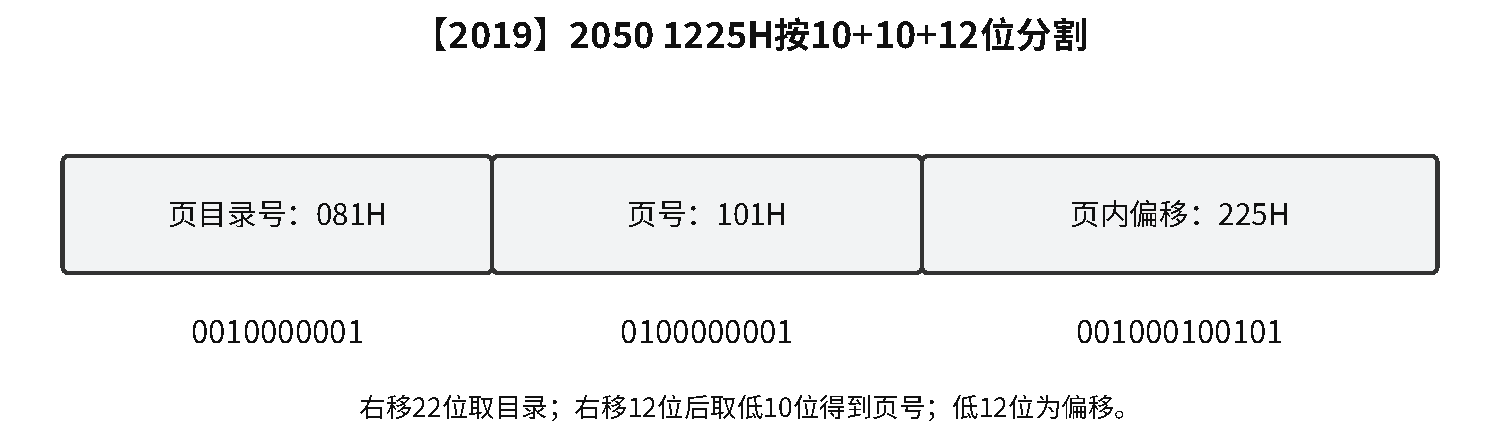
\includegraphics[width=0.95\textwidth,height=\textheight]{figures/OS_address_fields.pdf}
\caption{先按二进制位宽分割，再将每一段单独转为十六进制}\label{os-fig-address}
\end{figure}

\Needspace{6\baselineskip}

\textbf{解析。} 偏移为低 12 位 225H。目录号为地址右移 22 位，得 081H；下级页号为地址右移 12 位后取低 10 位，得 101H。答案为 \textbf{A}。若先把``205''当成某个字段，就把十六进制的 4 位分组误当成题设的 10 位字段。

\subsection{TLB 缓存的是转换，不是文件内容}\label{os-c05-h105}

\textbf{快表 TLB}缓存近期地址转换及相关权限信息。命中时直接得到页框和权限；未命中时遍历页表，找到有效映射后可填入 TLB。TLB 未命中只说明转换不在该缓存，页面仍可能在内存；页表项表明合法页面不驻留才可能引发缺页。数据 Cache 又缓存实际数据，不能把 TLB 命中当成数据已经在 Cache。

\noindent{}〖3.2-014〗 二级页表、TLB 命中率 75\%，忽略 TLB 查询时间，页表均在内存且不考虑缺页。命中访问一次数据内存；未命中需要两次读页表和一次读数据，故平均访存次数为 \(0.75\times1+0.25\times3=1.5\)。这里每个分支都含最后的数据访问，不能只计算两次查表。

若 TLB 查询耗时 \(t\)、一次主存访问耗时 \(m\)，并且二者串行，则上述平均时间为 \(t+1.5m\)。若题目给定 TLB 与其他硬件并行查询、页表遍历缓存或不同层次命中率，必须按相应路径重列分支，不能硬套同一公式。

\section{分段和段页式：先检查段内地址}\label{os-5-6}

\textbf{分段}按程序的逻辑单位划分地址空间，例如代码段、数据段、栈段，每段长度可不同。逻辑地址用``段号、段内偏移''表示；段表记录段基址、段长和保护等。段号要落在段表范围内，偏移要小于段长，权限要允许本次操作，然后才计算基址加偏移。

\textbf{段页式}先按逻辑意义分段，再把各段分页；段表指向本段页表，页表再映射页框。它用段组织逻辑单位，用页框安排物理存储，不是``先把物理内存分段，再统一分页''。

转换时先检查段号和段级权限，再按段表给出的页表长度检查段内页号，合法后才查该段页表。题设若另外给出以字节为单位的段长，还须检查完整段内偏移没有越界；末页存在于内存，不会自动取消这个段长限制。

\begin{longtable}[]{@{}
  >{\raggedright\arraybackslash}p{(\columnwidth - 6\tabcolsep) * \real{0.2176}}
  >{\raggedright\arraybackslash}p{(\columnwidth - 6\tabcolsep) * \real{0.2588}}
  >{\raggedright\arraybackslash}p{(\columnwidth - 6\tabcolsep) * \real{0.2480}}
  >{\raggedright\arraybackslash}p{(\columnwidth - 6\tabcolsep) * \real{0.2754}}@{}}
\toprule\noalign{}
\begin{minipage}[b]{\linewidth}\raggedright
比较维度
\end{minipage} & \begin{minipage}[b]{\linewidth}\raggedright
基本分页
\end{minipage} & \begin{minipage}[b]{\linewidth}\raggedright
基本分段
\end{minipage} & \begin{minipage}[b]{\linewidth}\raggedright
段页式
\end{minipage} \\
\midrule\noalign{}
\endhead
\bottomrule\noalign{}
\endlastfoot
划分依据和大小 & 系统规定的定长页，与程序逻辑模块无必然对应 & 代码、数据等逻辑单位，段长可变 & 先按逻辑分段，各段再分成定长页 \\
地址怎样解释 & 线性地址拆为页号、页内偏移 & 段号、段内偏移 & 段号、段内页号、页内偏移；后两项来自段内地址 \\
对程序的可见性 & 分页通常对程序透明 & 显式区分各逻辑段 & 段可见，段内分页通常透明 \\
物理连续性与碎片 & 页内连续，页间可离散；末页可能有内部碎片 & 每段连续，段间可离散；可能有外部碎片 & 每页内连续，同一段可跨离散页框；各段末页可能有内部碎片 \\
共享与保护 & 通过页映射和逐页权限实现 & 以完整逻辑段为单位较直观 & 段级逻辑组织与页级物理映射共同起作用 \\
基本地址转换路径 & 页表→目标单元 & 段表→目标单元 & 段表→本段页表→目标单元 \\
\end{longtable}

最后一行若按\textbf{单级页表、各表均在主存、没有 TLB 或其他缓存命中，也不发生缺页、越界或权限异常}计算，分别需要2、2、3次主存访问。改为多级页表或引入 TLB 后，应按实际路径重新计数。

\noindent{}【2016】 某进程段表如下，访问段号 2、段内地址 400 的逻辑地址，结果是（　）。

\begin{longtable}[]{@{}
  >{\raggedright\arraybackslash}p{(\columnwidth - 8\tabcolsep) * \real{0.1940}}
  >{\raggedright\arraybackslash}p{(\columnwidth - 8\tabcolsep) * \real{0.1940}}
  >{\raggedright\arraybackslash}p{(\columnwidth - 8\tabcolsep) * \real{0.2119}}
  >{\raggedright\arraybackslash}p{(\columnwidth - 8\tabcolsep) * \real{0.1940}}
  >{\raggedright\arraybackslash}p{(\columnwidth - 8\tabcolsep) * \real{0.2058}}@{}}
\toprule\noalign{}
\begin{minipage}[b]{\linewidth}\raggedright
段号
\end{minipage} & \begin{minipage}[b]{\linewidth}\raggedright
段长
\end{minipage} & \begin{minipage}[b]{\linewidth}\raggedright
内存起始地址
\end{minipage} & \begin{minipage}[b]{\linewidth}\raggedright
权限
\end{minipage} & \begin{minipage}[b]{\linewidth}\raggedright
状态
\end{minipage} \\
\midrule\noalign{}
\endhead
\bottomrule\noalign{}
\endlastfoot
0 & 100 & 6000 & 只读 & 在内存 \\
1 & 200 & --- & 读写 & 不在内存 \\
2 & 300 & 4000 & 读写 & 在内存 \\
\end{longtable}

A. 段缺失异常　　B. 内存地址 4400　　C. 越权异常　　D. 越界异常

段 2 虽驻留且可读写，但偏移 \(400\ge300\)，已经越界，答案为 \textbf{D}。必须先检查长度，不能直接得到 4400。这里的数字是题设地址单位，不必擅自加上 KB。

\section{请求分页：合法但不驻留时会发生什么}\label{os-5-7}

\textbf{局部性}是程序在一段时期内倾向反复访问某些对象或其相邻位置。时间局部性来自循环与重用，空间局部性来自顺序指令、数组邻近元素等。虚拟内存利用这种特征，只保留当前所需部分，并在需要时调入其他部分，不要求整个进程同时装入。

请求分页的页表项需要区分页面是否驻留，并记录调页所需位置与状态。存在位表示是否在内存；访问位帮助估计近期使用；修改位表示装入后是否被写过，关系到淘汰时是否必须回写。\textbf{修改位不是写权限位}：允许写但尚未写的页可以是可写且 M=0；只读保护检查则发生在实际写入前。

\begin{longtable}[]{@{}
  >{\raggedright\arraybackslash}p{(\columnwidth - 4\tabcolsep) * \real{0.2832}}
  >{\raggedright\arraybackslash}p{(\columnwidth - 4\tabcolsep) * \real{0.3413}}
  >{\raggedright\arraybackslash}p{(\columnwidth - 4\tabcolsep) * \real{0.3754}}@{}}
\toprule\noalign{}
\begin{minipage}[b]{\linewidth}\raggedright
比较维度
\end{minipage} & \begin{minipage}[b]{\linewidth}\raggedright
基本分页
\end{minipage} & \begin{minipage}[b]{\linewidth}\raggedright
请求分页
\end{minipage} \\
\midrule\noalign{}
\endhead
\bottomrule\noalign{}
\endlastfoot
执行前的驻留要求 & 按基本模型，待运行程序所需页面先装入内存 & 可先装入一部分，合法页面允许暂不驻留 \\
映射记录承担什么 & 给出页到页框的映射与相应保护信息 & 还需驻留状态、调页位置及置换所需的访问、修改等信息 \\
TLB 未命中以后 & 查主存页表取得已有映射 & 先查页表；驻留则继续，不驻留才进入缺页分支 \\
内存不足时怎样继续 & 不能只靠基本分页的地址变换解决 & 可能置换、必要时回写，再调入并更新映射 \\
本次指令怎样结束 & 正常转换后访问目标单元 & 缺页处理完成后重试原访存；异常处理费不能漏计 \\
\end{longtable}

TLB 是地址转换缓存，基本分页和请求分页都可以使用它；是否有 TLB 与是否允许缺页是两个维度。

一次访存的分支应顺着执行：检查地址合法性，查询 TLB/页表并检查存在状态与访问权限；合法但不驻留则引发缺页异常，内核定位后备内容，取得空闲页框或选择牺牲页；牺牲页若为脏页且需要保留则回写，调入所需页，更新页表和 TLB，重新执行被中断的访存。访问非法地址应按错误处理，不能一概``给它调一页''。

\begin{figure}
\centering
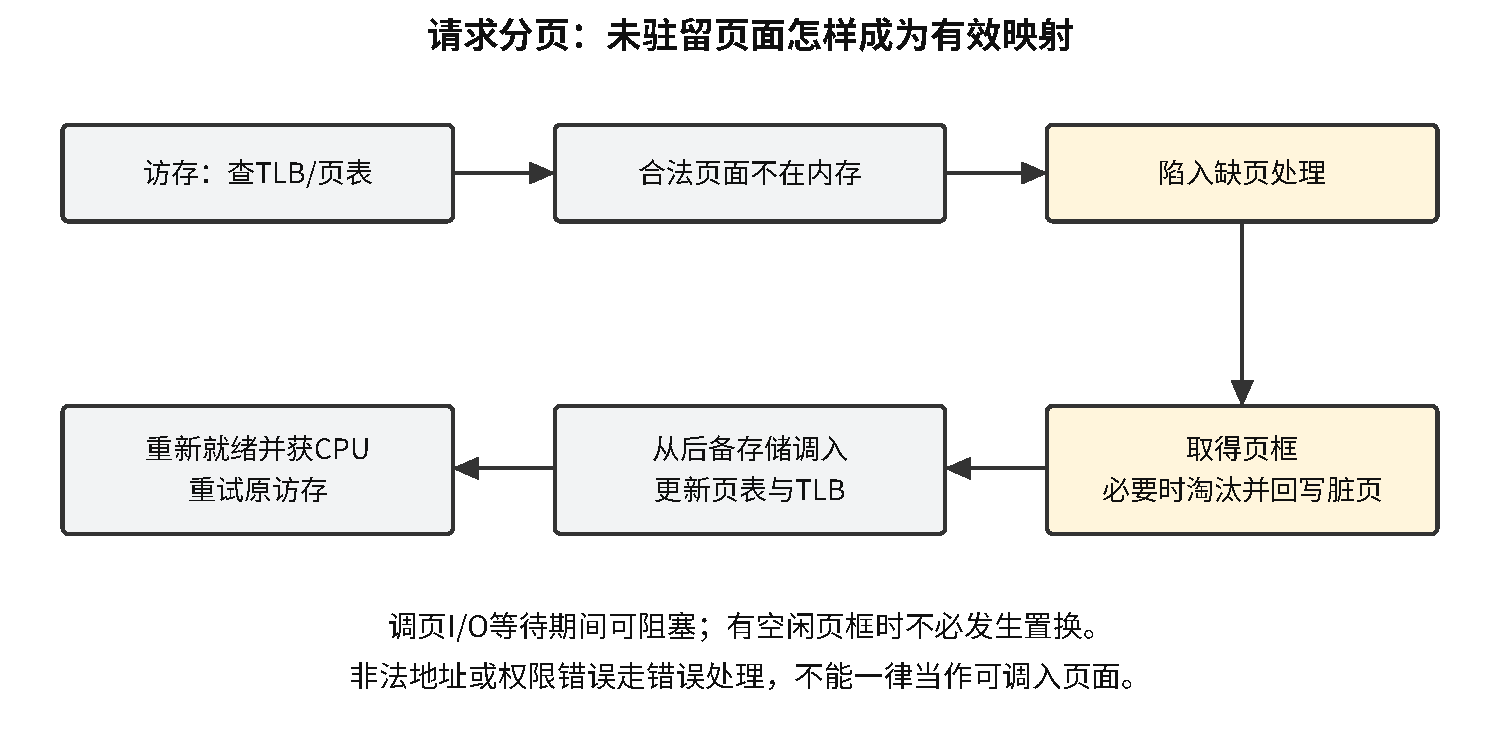
\includegraphics[width=0.95\textwidth,height=\textheight]{figures/OS_page_fault.pdf}
\caption{缺页处理会阻塞等待 I/O；页面就绪以后还要重试原访存}\label{os-fig-fault}
\end{figure}

缺页不一定发生置换：有空闲页框就可直接装入。反过来，一次复杂指令可能访问多个页面，执行期间可能产生不止一次缺页，系统必须保存足够的重启状态；最少页框数还受指令寻址方式等约束。页面置换算法不能弥补``一条指令所需页面无论如何无法同时提供''的基本执行条件。

\section{页框分配与置换范围}\label{os-5-8}

\textbf{驻留集}是进程当前在内存的页面集合。固定分配给进程固定数量页框；可变分配允许按运行状况调整。\textbf{局部置换}只在本进程驻留集中选牺牲页；\textbf{全局置换}可从其他进程等更大集合中选择，会改变各进程实际占有的页框量。

因此经典组合中，固定分配通常配局部置换；可变分配可以局部或全局置换。把固定分配与一般全局置换直接组合，会使被换出进程的页框量改变，违背这里``固定''的约定。分配可按平均、进程大小或优先级等方法进行，但还须满足体系结构要求的最少页框数。

请求调页在真正缺页时装入，能减少无用装入；预调页根据局部性提前带入可能需要的内容，可以减少后续等待，也可能调入没用的页。回写策略、清洁页缓冲和空闲页队列影响缺页处理代价，不能只盯着替换算法名称。

\section{页面置换：必须跟踪实际状态}\label{os-5-9}

\textbf{OPT}淘汰未来最长时间不再访问的页，未来不再访问者优先；它需要未来信息，主要用作比较基准。\textbf{FIFO}淘汰最早装入者，命中通常不改变装入顺序。\textbf{LRU}淘汰最近最久未使用者，每次命中也要更新最近使用关系。只在缺页时更新 LRU 次序，会把它错误地执行成接近 FIFO。

\subsection{例 5-5　缺页次数与置换次数相差初装入次数}\label{os-ex5-5}

\noindent{}【2019】 某系统采用 LRU 页置换和局部置换。为进程预分配 4 个页框，访问页号依次为 0、1、2、7、0、5、3、5、0、2、7、6。产生页面置换的总次数为（　）。

A. 3　　B. 4　　C. 5　　D. 6

\Needspace{6\baselineskip}

\textbf{解析。} 下表按``最久未用→最近使用''记驻留页，因而每次命中也会移动相应页的位置；开始页框为空。

\begin{longtable}[]{@{}
  >{\raggedright\arraybackslash}p{(\columnwidth - 4\tabcolsep) * \real{0.2762}}
  >{\raggedright\arraybackslash}p{(\columnwidth - 4\tabcolsep) * \real{0.3660}}
  >{\raggedright\arraybackslash}p{(\columnwidth - 4\tabcolsep) * \real{0.3576}}@{}}
\toprule\noalign{}
\begin{minipage}[b]{\linewidth}\raggedright
访问
\end{minipage} & \begin{minipage}[b]{\linewidth}\raggedright
访问后最近使用次序
\end{minipage} & \begin{minipage}[b]{\linewidth}\raggedright
结果
\end{minipage} \\
\midrule\noalign{}
\endhead
\bottomrule\noalign{}
\endlastfoot
0 & 0 & 缺页，空框装入 \\
1 & 0、1 & 缺页，空框装入 \\
2 & 0、1、2 & 缺页，空框装入 \\
7 & 0、1、2、7 & 缺页，空框装入 \\
0 & 1、2、7、0 & 命中 \\
5 & 2、7、0、5 & 缺页，淘汰 1 \\
3 & 7、0、5、3 & 缺页，淘汰 2 \\
5 & 7、0、3、5 & 命中 \\
0 & 7、3、5、0 & 命中 \\
2 & 3、5、0、2 & 缺页，淘汰 7 \\
7 & 5、0、2、7 & 缺页，淘汰 3 \\
6 & 0、2、7、6 & 缺页，淘汰 5 \\
\end{longtable}

共 9 次缺页，前 4 次利用空框，实际置换 5 次，答案为 \textbf{C}。题目问置换时，不要把所有缺页都记为替换。

\subsection{Clock 的访问位给页面第二次机会}\label{os-c05-h203}

基本 Clock 把页框排成环，指针指向下一个候选。页面被访问时置 A=1；缺页需替换时，检查指针所指页，A=0 就选它，A=1 则清为 0 并前进，直到选中牺牲页。新装入并被本次访问的页设 A=1，指针前移。指针初始位置、装入后位置若题设另有规定，要按题设执行。

\textbf{机制小例（原创）。} 四页框按环依次为 \(p,q,r,s\)，访问位为 1、0、1、0，指针从 p 开始。需淘汰时，先将 p 的 1 清 0，再选 q；r、s 本次未被扫描，原位不变。不能每次缺页都把所有访问位统一清零。这一小例只检查扫描中间状态，未替代真题的选页任务。

改进型 Clock 再考虑修改位。在本书采用的四类优先关系中，依次考虑 (A,M) 为 (0,0)、(0,1)、(1,0)、(1,1)：先选近期未访问且不需回写者，再考虑近期未访问的脏页，近期访问过者留待后续。具体多轮扫描会修改 A，必须按当时状态判断，不能用开扫描前的分类永久排名。

常见实现先一轮查 (0,0)，不修改 A；找不到，再查 (0,1)，并把经过但未选中的页的 A 清零；仍找不到则重做两轮。M 不能因扫描而任意清零，脏内容只有完成相应回写后才可变为干净。

\subsection{例 5-6　缺页后，旧页框字段不能直接沿用}\label{os-ex5-6}

\noindent{}【2021】 某请求分页系统页大小为 4 KB，按字节编址。为进程 P 分配 2 个固定页框，采用改进型 Clock，页表部分内容如下。

\begin{longtable}[]{@{}
  >{\raggedright\arraybackslash}p{(\columnwidth - 8\tabcolsep) * \real{0.2000}}
  >{\raggedright\arraybackslash}p{(\columnwidth - 8\tabcolsep) * \real{0.2000}}
  >{\raggedright\arraybackslash}p{(\columnwidth - 8\tabcolsep) * \real{0.2000}}
  >{\raggedright\arraybackslash}p{(\columnwidth - 8\tabcolsep) * \real{0.2000}}
  >{\raggedright\arraybackslash}p{(\columnwidth - 8\tabcolsep) * \real{0.2000}}@{}}
\toprule\noalign{}
\begin{minipage}[b]{\linewidth}\raggedright
页号
\end{minipage} & \begin{minipage}[b]{\linewidth}\raggedright
页框号
\end{minipage} & \begin{minipage}[b]{\linewidth}\raggedright
存在位
\end{minipage} & \begin{minipage}[b]{\linewidth}\raggedright
访问位
\end{minipage} & \begin{minipage}[b]{\linewidth}\raggedright
修改位
\end{minipage} \\
\midrule\noalign{}
\endhead
\bottomrule\noalign{}
\endlastfoot
2 & 20H & 0 & 0 & 0 \\
3 & 60H & 1 & 1 & 0 \\
4 & 80H & 1 & 1 & 1 \\
\end{longtable}

P 访问虚拟地址 02A01H，经地址变换得到的物理地址是（　）。

A. 00A01H　　B. 20A01H　　C. 60A01H　　D. 80A01H

\Needspace{6\baselineskip}

\textbf{解析。} 低 12 位偏移为 A01H，页号为 2。其存在位为 0，旧的 20H 不是这次可以直接使用的有效驻留映射。两个页框已被页 3、4 占据，需要置换；它们都被访问过，但页 3 干净、页 4 脏，按本题改进型 Clock 先淘汰页 3，把页 2 装到 60H 页框。于是物理地址为 \(60_H\times1000_H+A01_H=60A01_H\)，答案为 \textbf{C}。

若有空闲页框，则未必需要淘汰页 3；本题``固定 2 个且均已占用''决定了这一分支。若存在位本来为 1，则无须先执行同样的换页过程。

FIFO 可能出现 \textbf{Belady 异常}：增加页框反而增加缺页。LRU 与 OPT 具有相应栈性质，在相同引用串和一致初态下，增加页框不会使其缺页次数增加。不要把 FIFO 的异常推广成所有算法必有的现象，也不要把``LRU 通常利用局部性''写成对任意引用串必优于 FIFO。

\section{内存映射文件：把文件内容放入虚拟地址视图}\label{os-5-10}

\textbf{内存映射文件}把文件的某个范围与进程一段虚拟地址范围关联，程序通过访存访问映射内容，系统用分页等机制按需建立驻留页。它省去了应用反复显式调用读写并维护用户副本的某些工作，但不表示文件整体一次性进入物理内存，也不表示每次访存立即写到磁盘。

共享映射可让多个进程看到同一文件内容，因而支持进程间通信；对共享可写页的竞争仍须同步。私有映射的修改可通过写时复制保留为本进程私有，不必改原文件。页到文件块的后备关系由映射与文件系统共同维护，不能把它理解成绕过文件系统而直接把磁盘地址当内存地址。

映射以后仍受地址范围和权限约束，映射建立、页面驻留、写回持久化是不同事件。题目若问磁盘 I/O 次数，要检查页面是否已缓存、是否发生缺页、脏页是否回写，不能仅按源代码中的读写次数计算。

\section{工作集、抖动与平均访问时间}\label{os-5-11}

\textbf{工作集}是在给定窗口内实际访问过的不同页面的集合。若窗口按最近 \(\Delta\) 次引用定义，就从当前位置向前数 \(\Delta\) 次引用，再去重；不能先数 \(\Delta\) 个不同页。驻留集描述当前物理状态，工作集描述近期访问需求，工作集不必总是驻留集的子集：刚需要但尚未调入的页就可能属于需求而不驻留。

\subsection{例 5-7　窗口内有重复，集合只记一次}\label{os-ex5-7}

\noindent{}【2016】 某进程访问页面的序列如下，t 位于所示竖线处，尚未访问竖线右侧的 0。

\[\ldots,1,3,4,5,6,0,3,2,3,2\;\big|_{t}\;0,4,0,3,2,9,2,1,\ldots\]

工作集窗口大小为 6，则 t 时刻工作集为（　）。

A. \{6,0,3,2\}　　B. \{2,3,0,4\}　　C. \{0,4,3,2,9\}　　D. \{4,5,6,0,3,2\}

\Needspace{6\baselineskip}

\textbf{解析。} 向前取最近六次引用 6、0、3、2、3、2，去重为 \{6,0,3,2\}，答案为 \textbf{A}。集合无需保留重复次数，也不能从 t 向未来取数；把窗口理解成``六个不同页面''会错误扩大范围。

\textbf{抖动}指页面频繁换出又很快需要换入，大量时间花在换页，实际计算进展很少。若多进程工作集所需总页框超过可用内存，过度增加并发度可能引发抖动。减少活动进程、增加相关进程可用页框、依据工作集或缺页率调节分配，才能针对驻留不足；仅扩充磁盘交换区容量或提高某进程优先级，不自动提供它需要的页框。

\subsection{数组访问怎样变成页引用串}\label{os-c05-h259}

\noindent{}〖3.2-012〗 页框为 512 B，数组 \texttt{int\ a{[}128{]}{[}128{]}} 按行优先存放，代码已经驻留，数据只有 1 个页框。下列代码执行会产生多少次缺页？

\par\medskip\noindent
\begin{minipage}{\linewidth}
\begin{verbatim}
for (int i = 0; i < 128; i++)
    for (int j = 0; j < 128; j++)
        a[j][i] = 0;
\end{verbatim}
\end{minipage}\par\medskip

A. 1　　B. 2　　C. 128　　D. 16384

\Needspace{6\baselineskip}

\textbf{解析。} 按本题采用的 4 B 整数和数组按页对齐、数据初始未装入的模型，一行正好 \(128\times4=512\) B，占一页。内层循环 j 增加，访问的是不同的行，即依次跨页；一份数据页框只能留下刚访问的那一行。每次引用都换到另一行，下一列从第 0 行重新开始时它也早已被淘汰，因此 \(128\times128=16384\) 次，答案为 \textbf{D}。

这里缺页与置换算法无关，因为只有一个数据页框。若把内层访问改为 \texttt{a{[}i{]}{[}j{]}}，按行连续访问且上述对齐条件不变，每行初次访问缺页一次，总共 128 次。这是\textbf{原创变式}，只改变下标次序，用来检查空间局部性，而非另一道原题。若整数大小、初始驻留或数组页对齐改变，先重建地址和页引用串，再讨论算法，不能只背 16384。

\subsection{有效访问时间要列出所有分支}\label{os-c05-h275}

设不缺页的一次访问平均耗时为 \(T_0\)，缺页率为 \(p\)，一次缺页的完整分支平均耗时为 \(T_f\)，且 \(T_f\) 已包括调页、必要写回、处理程序及重试访问，则

\[E[T]=(1-p)T_0+pT_f.\]

若题目把缺页服务时间 \(D\) 定义成正常访存以外的附加开销，则可写 \(E[T]=T_0+pD\)，两种写法只是费用定义不同。TLB 命中率与缺页率也不能相加充当一个命中率；应按条件概率和完整路径分支。

\textbf{原创计算检查。} 若 \(T_0=100\) ns，缺页完整分支为 10 ms，希望平均访问不超过 200 ns，则

\[p\le\frac{200-100}{10^7-100}\approx10^{-5}.\]

毫秒先换成纳秒，才可与 100 相减。这个数量级说明为什么低缺页率仍可能显著影响时间，不是对任何实机性能的统计结论。

\subsection{例 5-8　一次缺页要把``失败、调页、重试''全部计时}\label{os-ex5-8}

\noindent{}【2009】 请求分页管理系统中，假设某进程的页表内容如下表所示。

\begin{longtable}[]{@{}
  >{\raggedright\arraybackslash}p{(\columnwidth - 4\tabcolsep) * \real{0.3128}}
  >{\raggedright\arraybackslash}p{(\columnwidth - 4\tabcolsep) * \real{0.3155}}
  >{\raggedright\arraybackslash}p{(\columnwidth - 4\tabcolsep) * \real{0.3716}}@{}}
\toprule\noalign{}
\begin{minipage}[b]{\linewidth}\raggedright
页号
\end{minipage} & \begin{minipage}[b]{\linewidth}\raggedright
页框号
\end{minipage} & \begin{minipage}[b]{\linewidth}\raggedright
有效位（存在位）
\end{minipage} \\
\midrule\noalign{}
\endhead
\bottomrule\noalign{}
\endlastfoot
0 & 101H & 1 \\
1 & --- & 0 \\
2 & 254H & 1 \\
\end{longtable}

页面大小为 4 KB，一次内存的访问时间为 100 ns，一次快表（TLB）的访问时间为 10 ns，处理一次缺页的平均时间为 \(10^8\) ns（已含更新 TLB 和页表的时间）。进程的驻留集大小固定为 2，采用最近最少使用置换算法（LRU）和局部淘汰策略。假设：①TLB 初始为空；②地址转换时先访问 TLB，若 TLB 未命中，再访问页表（忽略访问页表之后的 TLB 更新时间）；③有效位为 0 表示页面不在内存中，产生缺页中断，缺页中断处理后，返回到产生缺页中断的指令处重新执行。设有虚地址访问序列 2362H、1565H、25A5H，请问：

（1）依次访问上述三个虚地址，各需多少时间？给出计算过程。

（2）基于上述访问序列，虚地址 1565H 的物理地址是多少？请说明理由。

\Needspace{6\baselineskip}

\textbf{解析。} 4 KB=\(1000_H\) B，低 12 位是页内偏移。三个地址分别访问页 2、页 1、页 2，偏移依次为 362H、565H、5A5H。先连续跟踪这三个访问，不能把每个地址都从``TLB 为空''重新开始。

\begin{longtable}[]{@{}
  >{\raggedright\arraybackslash}p{(\columnwidth - 4\tabcolsep) * \real{0.2339}}
  >{\raggedright\arraybackslash}p{(\columnwidth - 4\tabcolsep) * \real{0.4411}}
  >{\raggedright\arraybackslash}p{(\columnwidth - 4\tabcolsep) * \real{0.3249}}@{}}
\toprule\noalign{}
\begin{minipage}[b]{\linewidth}\raggedright
本次访问
\end{minipage} & \begin{minipage}[b]{\linewidth}\raggedright
转换与驻留状态
\end{minipage} & \begin{minipage}[b]{\linewidth}\raggedright
耗时
\end{minipage} \\
\midrule\noalign{}
\endhead
\bottomrule\noalign{}
\endlastfoot
2362H & TLB 未命中；页 2 驻留，读页表后读目标内存；将页 2 的转换留在 TLB & \(10+100+100=210\) ns \\
1565H & TLB 未命中；页 1 不驻留；处理缺页，更新页表和 TLB；重试时命中 TLB，再读目标内存 & \(10+100+10^8+10+100=100000220\) ns \\
25A5H & 页 2 仍驻留，其转换仍在 TLB，直接命中后读目标内存 & \(10+100=110\) ns \\
\end{longtable}

第二次访问时两个页框已占满，需在本进程的页 0、页 2 中局部淘汰。页 2 刚被第一次访问使用，因此 LRU 选择页 0。将页 1 装入页框 101H，页 0 的存在位清零，并使其旧 TLB 转换失效；页 2 的映射不变。于是

\[PA(1565_H)=101_H\times1000_H+565_H=101565_H.\]

题目把页表、TLB 更新包含在 \(10^8\) ns 中，却明确要求返回原指令重试。因此更新成本不重复加，重试的 10+100 ns 仍须加。第三次访问能命中，也依赖连续执行所得的状态；TLB 未命中、缺页、页面置换是三个不同事件。

\subsection{例 5-9　数组偏移怎样逐级找到页表项}\label{os-ex5-9}

\noindent{}【2020】 某 32 位系统采用基于二级页表的请求分页存储管理方式，按字节编址，页目录项和页表项长度均为 4 字节，虚拟地址结构如下所示。

\begin{longtable}[]{@{}
  >{\raggedright\arraybackslash}p{(\columnwidth - 4\tabcolsep) * \real{0.3379}}
  >{\raggedright\arraybackslash}p{(\columnwidth - 4\tabcolsep) * \real{0.3126}}
  >{\raggedright\arraybackslash}p{(\columnwidth - 4\tabcolsep) * \real{0.3494}}@{}}
\toprule\noalign{}
\begin{minipage}[b]{\linewidth}\raggedright
页目录号（10 位）
\end{minipage} & \begin{minipage}[b]{\linewidth}\raggedright
页号（10 位）
\end{minipage} & \begin{minipage}[b]{\linewidth}\raggedright
页内偏移量（12 位）
\end{minipage} \\
\midrule\noalign{}
\endhead
\bottomrule\noalign{}
\endlastfoot
\end{longtable}

某 C 程序中数组 \texttt{a{[}1024{]}{[}1024{]}} 的起始虚拟地址为 1080 0000H，数组元素占 4 字节，该程序运行时，其进程的页目录起始物理地址为 0020 1000H。请回答下列问题。

（1）数组元素 \texttt{a{[}1{]}{[}2{]}} 的虚拟地址是什么？对应的页目录号和页号分别是什么？对应的页目录项的物理地址是什么？若该目录项中存放的页框号为 00301H，则 \texttt{a{[}1{]}{[}2{]}} 所在页对应的页表项的物理地址是什么？

（2）数组 a 在虚拟地址空间中所占的区域是否必须连续？在物理地址空间中所占区域是否必须连续？

（3）已知数组 a 按行优先方式存放，若对数组 a 分别按行遍历和按列遍历，则哪种遍历方式的局部性更好？

\Needspace{6\baselineskip}

\textbf{解析。} （1）C 的下标从 0 开始，按行优先存放。到 \texttt{a{[}1{]}{[}2{]}} 的字节偏移为 \((1\times1024+2)\times4=4104=1008_H\)，故其虚拟地址为

\[1080\,0000_H+1008_H=1080\,1008_H.\]

然后按位宽拆分，并把``表项地址''和``表项中保存的页框号''分开计算。

\begin{longtable}[]{@{}
  >{\raggedright\arraybackslash}p{(\columnwidth - 4\tabcolsep) * \real{0.3322}}
  >{\raggedright\arraybackslash}p{(\columnwidth - 4\tabcolsep) * \real{0.3831}}
  >{\raggedright\arraybackslash}p{(\columnwidth - 4\tabcolsep) * \real{0.2845}}@{}}
\toprule\noalign{}
\begin{minipage}[b]{\linewidth}\raggedright
所求对象
\end{minipage} & \begin{minipage}[b]{\linewidth}\raggedright
计算
\end{minipage} & \begin{minipage}[b]{\linewidth}\raggedright
结果
\end{minipage} \\
\midrule\noalign{}
\endhead
\bottomrule\noalign{}
\endlastfoot
页目录号 & \(VA\gg22\) & 042H \\
页号（下级表索引） & \((VA\gg12)\mathbin{\&}3FF_H\) & 001H \\
页内偏移 & \(VA\mathbin{\&}FFF_H\) & 008H \\
页目录项物理地址 & \(0020\,1000_H+042_H\times4\) & 0020 1108H \\
下级页表起始物理地址 & \(00301_H\times1000_H\) & 0030 1000H \\
页表项物理地址 & \(0030\,1000_H+001_H\times4\) & 0030 1004H \\
\end{longtable}

题目没有给出这个页表项中的最终页框号，不能把 0030 1004H 当作 \texttt{a{[}1{]}{[}2{]}} 的物理地址；它是下一步需要读取的映射项的位置。

（2）该 C 数组的元素按规定连续排列，所以所占虚拟区域必须连续；相邻虚拟页可映射到离散的页框，物理区域不必连续。页内连续与跨页离散可以同时成立。

（3）每行 \(1024\times4=4096\) B，恰为一页，起始地址也按页对齐。按行遍历在同一页中连续取元素，空间局部性更好；按列遍历的相邻元素相差 4096 B，会逐行跨页。但原题没有给驻留集大小、替换规则和初始状态，不能进一步声称按列必然每次缺页。地址跨度决定访问模式，缺页次数还取决于驻留状态。

\section{自测：先写地址字段和状态，再计算}\label{os-5-review}

以下为原创回顾设问。

\begin{enumerate}
\def\labelenumi{\arabic{enumi}.}
\tightlist
\item
  32 位虚拟地址、4 KB 页、4 B 页表项，单级页表若覆盖全部空间，需要多少表项和多少字节？
\item
  TLB 未命中而页表存在位为 1，是否一定访问磁盘？存在位为 1、写权限为 0，写访问应怎样处理？
\item
  某页修改位为 0，是否表示程序没有读过该页？
\item
  例5-5中为何 9 次缺页只有 5 次置换？
\item
  工作集窗口增加，集合大小是否每次恰好增加 1？
\end{enumerate}

\subsection{自测答案}\label{os-c05-h365}

\begin{enumerate}
\def\labelenumi{\arabic{enumi}.}
\tightlist
\item
  页号 20 位，共 \(2^{20}\) 项，占 \(2^{22}\) B，即 4 MB；这与物理页框总数不是同一个计算。
\item
  未命中可通过主存页表取得映射，不必读盘。写权限不足应触发保护异常，不能当作普通缺页调入后允许写。
\item
  否。读访问可以使访问位置 1，却不使修改位置 1。
\item
  最初四次使用空闲页框，尚未淘汰任何页；之后满框缺页才置换。
\item
  不会。新纳入的一次引用可能已在集合中，窗口内重复引用只算同一个页。
\end{enumerate}

\chapter{文件、目录与文件系统}\label{os-ch6}

文件系统把``按名称找到数据''分成几步：由路径查目录项，由目录项找到文件控制信息，再把文件内偏移转换成存储块位置。目录、索引节点、打开文件表和数据块分别承担不同工作，不能把它们都叫作``文件的信息''而混算访问次数。

本章文件内字节偏移和逻辑块号从 0 开始；``第几个记录''若采用自然序号则从 1 开始。除题目另有定义，1 KB 为 1024 B。计算访盘次数时，逐次说明哪个目录块、索引块或数据块尚不在内存；已缓存的内容不重复计入。

\section{文件、文件控制块与索引节点}\label{os-6-1}

\textbf{文件}是具有名称和一定属性的持久数据集合。从使用者看，它可以是字节流，也可以由记录组成；从存储看，它最终占据若干物理块。文件的名称与内容不是同一个对象，一个文件可以通过多个名称被访问。

\textbf{文件控制块 FCB}是系统描述和管理文件的数据结构，通常记录类型、大小、所有者、权限、时间和存储位置等元数据。将文件名与其他描述信息分离时，目录项可只保留``文件名---索引节点号''，其余信息由\textbf{索引节点 inode}保存。inode 是这种设计中的文件控制信息载体，不是文件数据块，也不只是``指向文件的一个指针''。

索引节点号的意义局限于相应文件系统，不能只凭两个分区上的编号相同就判断是同一个文件。内存中的 inode 还可包含运行时锁、引用计数等；它与磁盘中持久保存的 inode 相关，但字段不必完全相同。

目录本身也是文件，其中存放的是用于查找对象的目录项；普通文件的数据内容不因为名字出现在目录中，就都存入目录。采用 inode 的模型还应区分三个位置：名字在目录项中，属性和块地址在 inode 中，用户内容在数据块中。

\begin{longtable}[]{@{}
  >{\raggedright\arraybackslash}p{(\columnwidth - 6\tabcolsep) * \real{0.2106}}
  >{\raggedright\arraybackslash}p{(\columnwidth - 6\tabcolsep) * \real{0.2678}}
  >{\raggedright\arraybackslash}p{(\columnwidth - 6\tabcolsep) * \real{0.2373}}
  >{\raggedright\arraybackslash}p{(\columnwidth - 6\tabcolsep) * \real{0.2842}}@{}}
\toprule\noalign{}
\begin{minipage}[b]{\linewidth}\raggedright
对象
\end{minipage} & \begin{minipage}[b]{\linewidth}\raggedright
记录什么
\end{minipage} & \begin{minipage}[b]{\linewidth}\raggedright
由什么找到它
\end{minipage} & \begin{minipage}[b]{\linewidth}\raggedright
何时改变或回收
\end{minipage} \\
\midrule\noalign{}
\endhead
\bottomrule\noalign{}
\endlastfoot
目录项 & 当前目录内的名字及 inode 号 & 逐层解析路径、查找所在目录 & 建立、重命名、增删链接时改变；关闭文件不删除它 \\
磁盘 inode & 文件类型、大小、权限、链接数、数据块地址等持久信息 & 在本文件系统解释 inode 号 & 文件内容或属性改变时更新；须满足无链接、无有效使用引用等回收条件 \\
内存 inode & 已载入的文件信息及运行时锁、引用状态等 & inode 缓存或打开对象引用 & 可由多个打开者共享；无打开者后是否立即释放取决于缓存模型 \\
打开实例与进程描述符表 & 打开实例记录文件位置、访问方式；进程表把 fd 关联到实例 & 已返回的 fd 在所属进程内解释 & open 建立，dup 或继承可共享实例，close 释放相应引用 \\
\end{longtable}

因此``知道文件名''``知道 inode 号''``inode 已在内存''和``数据已缓存''依次消除了不同查找步骤。访盘题要把题设明确命中的对象从路径中删去，不能由其中一个条件推得其他对象也都在内存。

\section{建立、打开、读写、关闭与删除}\label{os-6-2}

\textbf{建立文件}要分配文件控制信息，在父目录增加名字与文件标识的关联，并按规则初始化属性；空文件可以暂不分配实际数据块。\textbf{打开文件}按路径查找、检查权限，在内存建立或引用打开状态，返回文件描述符。打开不等于把整个文件内容读入内存。

一个常用抽象分为三层：进程文件描述符表把小整数 \texttt{fd} 指向打开实例；打开实例保存本次打开的状态，例如当前文件位置和访问方式；内存 inode 保存文件本身的共享属性及定位信息。不同教材有时把后两层合称系统打开文件表，本书计算前会按字段所属说明，避免因表名不同把状态混在一起。

\texttt{read(fd,}\allowbreak{}\texttt{buf,}\allowbreak{}\texttt{n)} 根据打开状态和当前偏移找到目标数据，必要时发起 I/O，向用户区返回实际读到的字节，并更新相应文件位置。\texttt{write} 可能分配新块、改变大小、把缓存标记为脏；返回成功不必表示数据已立即持久化到盘片。文件结束、短读、权限错误等应按题给语义处理。

\textbf{关闭}释放本次打开引用，必要时更新元数据；它不等于删除文件。\textbf{删除名字}从目录取消关联，硬链接计数随之变化；文件内容何时真正回收，还要检查是否仍有其他硬链接或有效打开引用。两类计数含义不同：磁盘硬链接数统计名字关联，打开引用数统计运行中的使用关系。

\subsection{例 6-1　最后关闭，释放的是哪一层}\label{os-ex6-1}

\noindent{}【2023】 若文件 F 仅被进程 P 打开并访问，则当进程 P 关闭 F 时，文件系统需要完成的是（　）。

A. 删除目录文件中 F 的目录项

B. 释放 F 的索引节点所占的内存空间

C. 释放 F 的索引节点所占的外存空间

D. 将文件磁盘索引节点中的链接计数减 1

\Needspace{6\baselineskip}

\textbf{解析。} 按本题最后关闭时释放相应内存控制信息的简化模型，答案为 \textbf{B}。A、C 属于删除持久对象的工作，D 对应硬链接关系改变；关闭并不取消文件名。实际系统可以把暂时没有打开者的 inode 留在缓存里，缓存回收时机与本题抽象不同，不能据此把 close 与 unlink 混为一谈。

\subsection{文件位置可以共享，也可以独立}\label{os-c06-h50}

两个进程分别 \texttt{open} 同一文件，通常得到两个打开实例，各有自己的文件位置，最后都指向同一文件的 inode。通过 \texttt{dup} 或进程继承共享同一打开实例时，文件位置也可能共享。因此``同一个文件''不决定读写位置是否相同；先看是否同一次打开的引用。

多个进程以写方式打开同一文件，不表示文件系统自动满足应用所需的完整事务互斥。要防止记录被交错修改，应使用规定的锁或其他同步方式。系统对单次写的原子性规则也不能任意推广为整个``读---修改---写''序列的原子性。

\section{文件保护：用户类别与权限组合}\label{os-6-3}

保护回答谁能对对象执行什么操作。口令、加密和访问控制各有作用，不能相互替代：加密保护内容可读性，访问控制由系统按身份与权限限制操作；读权限、写权限、执行权限也不同于调度优先级。

访问矩阵以主体为行、对象为列，格中保存允许操作集合。按对象列存放形成访问控制表 ACL，便于查``谁能使用这个文件''；按主体行组织授权可形成能力表一类机制，便于查``这个主体能用哪些对象''。保护还涉及授权、撤销和检查时机，不能只把权限存进去而在访问时不检查。

\subsection{例 6-2　权限可以同时成立，不能只编码一种}\label{os-ex6-2}

\noindent{}【2017】 某文件系统针对每个文件，把用户分成安全管理员、文件主、文件主的伙伴、其他用户 4 类；访问权限有完全控制、执行、修改、读取、写入 5 种。若 FCB 中用二进制位串表示不同类别用户对一个文件的访问权限，至少需要多少位？

A. 5　　B. 9　　C. 12　　D. 20

\Needspace{6\baselineskip}

\textbf{解析。} 对一类用户，五种权限可分别有或没有，需要 5 个独立二进制位。四类用户分别保存其权限组合，需要 \(4\times5=20\) 位，答案为 \textbf{D}。用 2 位编码用户类别、3 位编码一种操作，只能表达``是哪一类、做哪一种''，不能同时记录这个文件对全部四类用户开放的全部权限组合。题目未给权限之间必然蕴含关系，因此不能因``完全控制''这个名称擅自压缩其他位。

\section{逻辑结构：字节流和记录怎样被使用}\label{os-6-4}

\textbf{无结构文件}向应用提供字节序列，记录边界由应用自行解释；所谓无结构不是没有字节顺序。\textbf{有结构文件}由记录组成，可以定长或变长。定长记录且不跨块时，记录位置容易由长度计算；变长记录需要额外的边界、长度或索引信息。

顺序文件按记录次序存放，适合顺序处理；按关键字组织的顺序文件可利用有序性查找，但插入维护可能较贵。索引文件为记录或记录组维护索引，便于定位；索引顺序文件把顺序组织与索引结合。这些是应用看到或逻辑层规定的记录组织，和下面``一个文件的物理块连续、链接还是索引分配''不是同一维度。

例如变长记录文件可以用一个逻辑索引定位记录所在字节范围，文件本身再通过物理索引块定位磁盘块。两个``索引''服务不同层次，题目问哪个对象的空间、哪个访问链，就沿对应关系计算。

\section{物理分配：连续、链接与索引}\label{os-6-5}

\textbf{连续分配}记录起始块与长度，逻辑块 \(k\) 直接映射为起始块加 \(k\)，顺序和随机访问都容易；但文件增长可能受相邻空间限制，空闲空间也可能有外部碎片。按区段扩展可缓解增长问题，但不是每个文件永远只有一个连续区间。

\textbf{隐式链接分配}在各数据块内保存后继块号，目录记录首块等信息。逻辑上连续的数据可散在任意物理块；增长容易、无需一个大连续洞，但要找后面的块通常必须沿链读取，链指针也占用空间。损坏一个指针会影响后续定位。

\textbf{显式链接分配}把后继关系集中到文件分配表 FAT。表若驻留内存，沿链查找不必每步读取数据块，但定位第 \(k\) 个簇仍要执行链追踪，不等于具有直接随机下标。FAT 一般为每个受管簇保存一项，规模取决于受管卷的簇数；不能单凭某个文件最大长度就一般性推出整个卷的 FAT 大小，除非题目另外限定两者关系。

\textbf{索引分配}为文件记录各逻辑块的物理块号，可单级、多级或混合索引。根据逻辑块号查相应索引项即可定位，支持随机访问；索引本身占空间，小文件使用大索引块时可能浪费。UNIX 式混合索引让小文件直接索引，大文件逐渐使用间接层级。

比较访盘次数时，先统一起点：逻辑块号 \(k\) 从0开始，目录项或 inode 已在内存，查找路径上的数据块和索引块均未缓存，也没有预存的中间块号；FAT 行另假定分配表已驻留内存。

\begin{longtable}[]{@{}
  >{\raggedright\arraybackslash}p{(\columnwidth - 8\tabcolsep) * \real{0.1827}}
  >{\raggedright\arraybackslash}p{(\columnwidth - 8\tabcolsep) * \real{0.2098}}
  >{\raggedright\arraybackslash}p{(\columnwidth - 8\tabcolsep) * \real{0.2016}}
  >{\raggedright\arraybackslash}p{(\columnwidth - 8\tabcolsep) * \real{0.1986}}
  >{\raggedright\arraybackslash}p{(\columnwidth - 8\tabcolsep) * \real{0.2071}}@{}}
\toprule\noalign{}
\begin{minipage}[b]{\linewidth}\raggedright
分配方式
\end{minipage} & \begin{minipage}[b]{\linewidth}\raggedright
怎样定位第 \(k\) 个逻辑块
\end{minipage} & \begin{minipage}[b]{\linewidth}\raggedright
读取目标块需访盘
\end{minipage} & \begin{minipage}[b]{\linewidth}\raggedright
额外组织空间
\end{minipage} & \begin{minipage}[b]{\linewidth}\raggedright
增长与碎片
\end{minipage} \\
\midrule\noalign{}
\endhead
\bottomrule\noalign{}
\endlastfoot
连续 & 起始块号加 \(k\)，可直接定位 & 1次 & 起始块号、长度等描述信息 & 扩展受相邻空间制约；可能有外部碎片 \\
隐式链接 & 从首块读取后继指针，逐块追踪 & \(k+1\) 次 & 数据块中的后继指针 & 可离散追加；无外部碎片 \\
显式链接 FAT & 在内存表中追踪 \(k\) 条链接，再读目标块 & 1次，但仍有内存追链开销 & 全卷每簇的表项；驻留表占内存 & 可离散追加；受空闲簇及表规模约束 \\
单级、多级或混合索引 & 按块号确定索引项，逐级取得下层块号 & 经 \(h\) 级间接索引时 \(h+1\) 次；直接指针为1次 & 文件的索引项和索引块 & 可离散追加；范围受各级索引容量限制 \\
\end{longtable}

FAT 支持不读取前面数据块而访问指定块，这正是它相对隐式链接的优势；这不表示块号转换变成常数次内存访问。``无外部碎片''也不表示最后一个数据块一定装满，各方式仍可能留下块内未用空间。题目改变 inode、FAT 或索引块的缓存条件时，先删去已命中的那一级访问，再计总数。

\subsection{例 6-3　混合索引中，一次访问要经过几层}\label{os-ex6-3}

\noindent{}【2015】 文件索引节点中有 10 个直接索引指针，一级和二级索引指针各 1 个。磁盘块为 1 KB，每个索引指针 4 B。某文件索引节点已在内存，把该文件偏移量为 1234 和 307400（按字节编址）处所在的磁盘块读入内存，需要访问的磁盘块个数分别是（　）。

A. 1、2　　B. 1、3　　C. 2、3　　D. 2、4

\begin{figure}
\centering
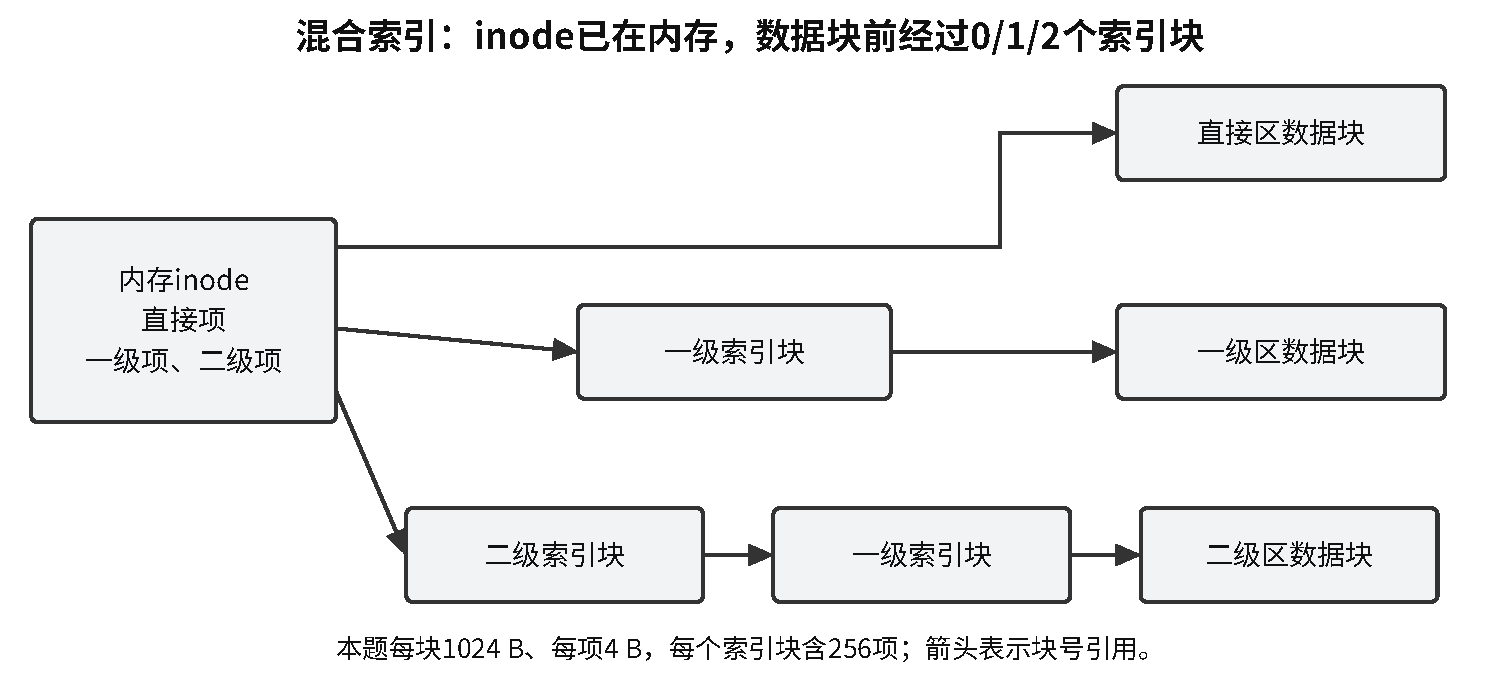
\includegraphics[width=0.95\textwidth,height=\textheight]{figures/OS_file_index.pdf}
\caption{直接、一级、二级路径经过的索引块数不同；图中只画少量代表项}\label{os-fig-index}
\end{figure}

\Needspace{6\baselineskip}

\textbf{解析。} 一个索引块能存 \(1024/4=256\) 项。直接索引覆盖前 10 KB；一级间接再覆盖 256 KB；二级间接再覆盖 \(256^2\) KB。

1234 小于 \(10\times1024\)，属于直接区。inode 已在内存，可直接取目标块号，只读 1 个数据块。307400 大于 \((10+256)\times1024=272384\)，进入二级区；需读二级索引块、对应的一级索引块和数据块，共 3 次，答案为 \textbf{B}。

还可定位到项：\(307400=300\times1024+200\)，逻辑块号 300；减去前面的 \(10+256=266\) 块，二级区内偏移 34 块，即先取二级索引的第 0 项，再取其所指索引块的第 34 项。块内偏移 200 不影响要经过的索引层数。

本题结构能表示的数据长度为 \((10+256+256^2)\times1024\) B，即 64 MB + 266 KB；其中不把索引块计为文件用户数据长度。若索引块已经缓存，访盘次数会减少；若 inode 尚不在内存，还应计入取得它的相应访问。题目说``索引节点已在内存''，不能再加一次 inode 读盘。

\subsection{例 6-4　链接文件修改一条记录，要把读和写都计入}\label{os-ex6-4}

\noindent{}〖4.2-025〗 一个记录文件采用隐式链接分配，定长逻辑记录为 100 B，采用记录成组分解，盘块为 512 B。目录项已读入内存，对第 22 个逻辑记录完成修改，共启动磁盘多少次？

A. 3　　B. 4　　C. 5　　D. 6

\Needspace{6\baselineskip}

\textbf{解析。} 按原题记录不跨块、每块容纳 5 条记录的模型，第 1---5 条在第 1 块，依次类推，第 22 条位于第 5 块。隐式链要从第 1 块沿后继指针读到第 5 块，共读 5 次，再把修改后的第 5 块写回 1 次，总计 6 次，答案为 \textbf{D}。目录已在内存只免去目录读取，不能免去沿链的数据块读取。

盘块中的链接指针若占用部分字节，本题只要每块剩余空间仍足够容纳 5 条 100 B 记录，结论不变；若允许跨块记录、索引已缓存或采用 FAT，则必须改画访问路径。不要把``修改第 22 条''理解成写 22 次，也不要漏掉最后的回写。

\section{目录和路径解析：逐层找到名字}\label{os-6-6}

单级目录把所有文件名放在一张表，简单但命名冲突多；两级目录按用户分开，缓解重名但共享和多层分类受限；树形目录让目录内再有子目录，便于按层次组织。绝对路径从根开始，相对路径从当前工作目录开始；\texttt{.} 表示当前目录，\texttt{..} 表示父目录，在权限与挂载规则允许的范围内解析。

访问 \texttt{/home/u/a.txt} 不能在一张全局名字表中凭空跳到数据。典型 inode 模型先从根目录查 \texttt{home}，取得其 inode，再查 \texttt{u}，最后在该目录中查 \texttt{a.txt} 并取得文件 inode。各层目录、inode、数据是否缓存，决定实际 I/O 数；路径分量的数量本身不是总访盘次数。

采用``名字与 inode 分离''可以使目录项更小，一块容纳更多名字，从而减少线性查找的目录块数。以王道书 §4.2 的目录模型为例，3200 项、每项 16 B、每块 1024 B，需要 50 个目录块。若目标等概率落在任意一项，且逐块线性查找，各块恰有相同数量目录项，则平均读取 \((1+50)/2=25.5\) 个目录块；随后再读 1 个 inode 块，总期望 26.5 次。用 \(50/2+1=26\) 是``大量目录块''的近似，不能当作相同概率模型下的精确值。

若目录使用哈希或树索引，查找次数应按相应结构计算；若预先只读入目录的一部分，也不能把剩余查找都视为零成本。当前工作目录使常用路径可以省去重复解析共同前缀，但不取消权限检查。

\section{硬链接、软链接与什么时候回收文件}\label{os-6-7}

\textbf{硬链接}是另一个目录项直接指向同一文件 inode；多个名字地位相同，不存在``原名字一删，另一个就失效''的必然关系。增加一个硬链接通常增加 inode 的硬链接计数，删除一个名字减少计数；计数归零且不再有有效使用引用等条件满足后，才能回收数据和 inode。硬链接通常不能跨文件系统，因为 inode 编号必须在本文件系统解释；通常也限制用户为目录建立硬链接，以避免目录环等管理问题。

\textbf{软链接或符号链接}是一个特殊文件，内容保存目标路径。访问它时再解析该路径；目标被删或移走后，软链接本身仍可存在，只是成为悬空链接。它可以跨文件系统，也可指向目录；相对目标路径的解释与链接所在位置有关，不能一概按调用者当前工作目录处理。

\begin{figure}
\centering
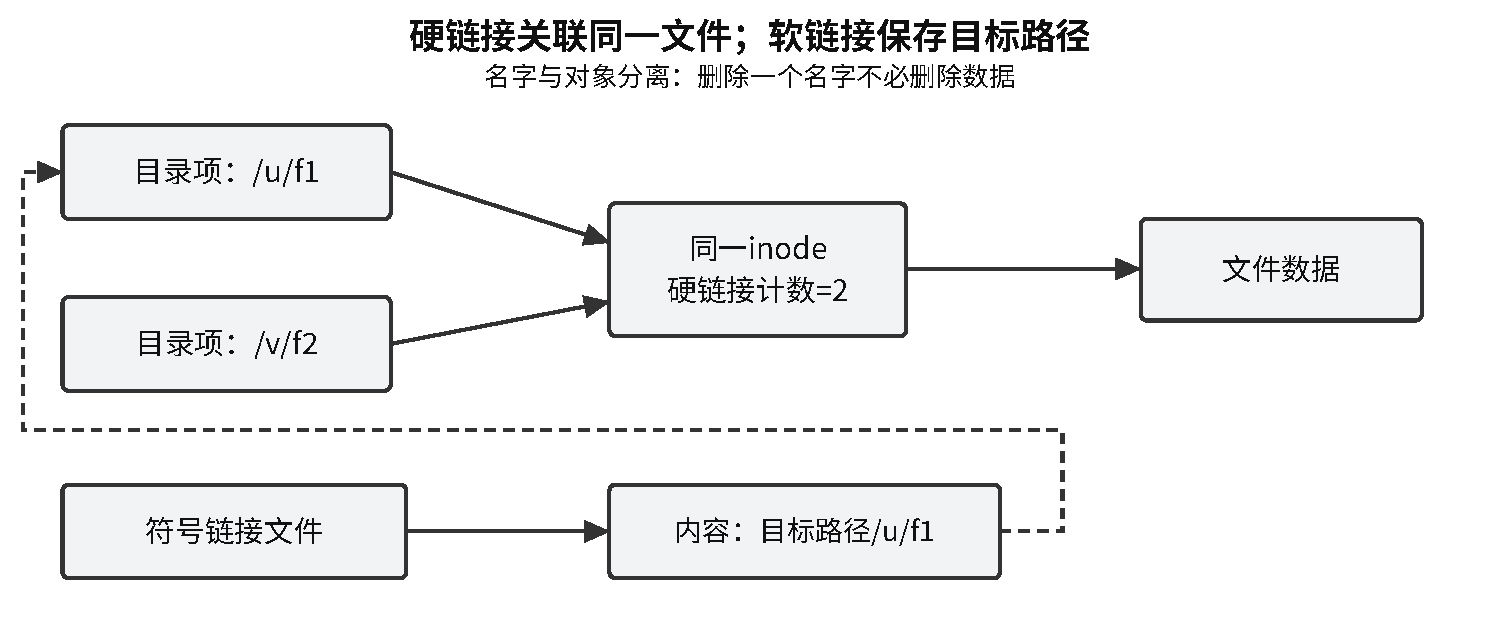
\includegraphics[width=0.95\textwidth,height=\textheight]{figures/OS_file_links.pdf}
\caption{两个硬链接指向同一 inode；软链接保存路径，经过名称解析再找到目标}\label{os-fig-links}
\end{figure}

\subsection{例 6-5　同一 inode 不要求同一读写位置}\label{os-ex6-5}

\noindent{}【2017】 若文件 f1 的硬链接为 f2，两个进程分别打开 f1、f2，获得文件描述符 fd1、fd2，则正确的是（　）。

Ⅰ. f1 和 f2 的读写指针位置保持相同

Ⅱ. f1 和 f2 共享同一个内存索引节点

Ⅲ. fd1 和 fd2 分别指向各自的用户打开文件表中的一项

A. 仅Ⅲ　　B. 仅Ⅱ、Ⅲ　　C. 仅Ⅰ、Ⅱ　　D. Ⅰ、Ⅱ、Ⅲ

\Needspace{6\baselineskip}

\textbf{解析。} f1、f2 是同一文件的两个名字，两次打开最终引用同一个 inode，Ⅱ正确。两进程分别打开，读写位置可以独立，Ⅰ错误。每个文件描述符在相应进程的描述符表中解释，分别关联各自的打开表项，Ⅲ正确。答案为 \textbf{B}。这与共享同一个打开实例的继承或复制描述符情形不同。

\section{文件系统的磁盘结构与内存结构}\label{os-6-8}

磁盘上的引导控制信息用于启动；卷控制块或超级块记录块大小、卷规模、空闲管理等总体信息；目录和 inode 区描述对象与名字；数据区保存内容。具体文件系统可采用其他布局，题目若给不同结构，应以其字段为准。不能把每个文件的所有索引都放入超级块。

挂载后，内存中维护已挂载文件系统信息、目录缓存、inode 缓存、系统打开对象以及进程描述符表等。缓存加快访问，却要求修改与持久化有规则。一次文件扩展可能同时修改数据块、空闲位图、inode 大小和块地址；若只写了一部分就断电，会出现泄漏或结构不一致。

一致性检查可以扫描目录、inode 与块使用关系，找出不一致；日志机制先记录需要完成的更新，再按规则提交和重放，减少崩溃后恢复工作。日志不表示任意用户数据都自动获得完整事务语义，其保证取决于记录元数据还是数据、提交和写回的具体规则。此处用于解释多结构更新的因果，不扩展为某种文件系统的实现手册。

\section{空闲空间：位图、空闲链和成组链接}\label{os-6-9}

\textbf{空闲表}记录连续空闲区的起点与长度，适合按区段管理；\textbf{空闲链}把空闲块或空闲区串起来；\textbf{位图}为每个受管块保留一位，值表示空闲或占用，具体 0、1 意义由题目规定；\textbf{成组链接}把若干空闲块号存成一组，用组内的连接信息指向后续组，并在内存保留当前组的块号栈。

位图大小主要由受管总块数决定，不随当前空闲块数改变；空闲表、空闲链所需内容则与当前空闲分布相关。成组链接是用少量组连接组织大量空闲块号，不是把所有文件的数据链混在一起。

\subsection{例 6-6　先定位位图块，再定位块内字节}\label{os-ex6-6}

\noindent{}【2015】 文件系统用位图表示磁盘空间分配，位图存于磁盘 32---127 号块，每块 1024 B，盘块和块内字节都从 0 编号。释放盘块号 409612 时，要修改的位所在盘块号和块内字节序号分别为（　）。

A. 81、1　　B. 81、2　　C. 82、1　　D. 82、2

\Needspace{6\baselineskip}

\textbf{解析。} 每个盘块的位图可表示 \(1024\times8=8192\) 个数据块。\(409612=50\times8192+12\)，故目标位在位图第 50 块，即磁盘块 \(32+50=82\)；余下第 12 位在块内字节 \(\lfloor12/8\rfloor=1\)，该字节中的位序号为 4。答案为 \textbf{C}。

位图自身的起始磁盘块号 32，只在``位图内相对块号''算出以后加；不能先把受管盘块号减去 32。修改成 0 还是 1，要看位图的空闲值约定，本题只问位置，不需要擅定。

\section{虚拟文件系统与挂载}\label{os-6-10}

\textbf{虚拟文件系统 VFS}为不同具体文件系统提供共同的操作抽象，把打开、查找、读写等请求通过相应操作接口分派给具体实现。统一接口不表示磁盘格式也统一，更不要求所有设备保存相同的 inode 布局。

Linux 式抽象常区分超级块对象、inode 对象、目录项对象 dentry 和文件对象：前者描述一个已挂载文件系统，inode 描述文件本体，dentry 缓存名字与父目录等关系，file 对象描述一次打开。dentry 与 inode 不是同一个英文术语；目录项对象的名称不能误写成 inode 对象。

\textbf{挂载}把某文件系统的根关联到现有名称空间的一个挂载点，使路径解析到该处时转入新文件系统。挂载点之下原有内容不因此被删除，只是在相应名称解析视图下被新挂载内容遮住。卸载要处理尚在使用的对象和待写回信息，不能只删一个路径字符串就认为设备已经可以安全移除。

\section{综合例题：目录、索引与容量共同约束}\label{os-6-11}

\subsection{例 6-7　同一索引节点怎样连接目录查找与文件扩展}\label{os-ex6-7}

\noindent{}【2022】 某文件系统的磁盘块大小为 4 KB，目录项由文件名和索引节点号构成，每个索引节点占 256 字节，其中包含直接地址项 10 个，一级、二级和三级间接地址项各 1 个，每个地址项占 4 字节。该文件系统中子目录 stu 的结构如下图所示，stu 包含子目录 course 和文件 doc，course 子目录包含文件 course1 和 course2。各文件的文件名、索引节点号、占用磁盘块的块号如图中表所示。请回答下列问题。

\begin{figure}
\centering
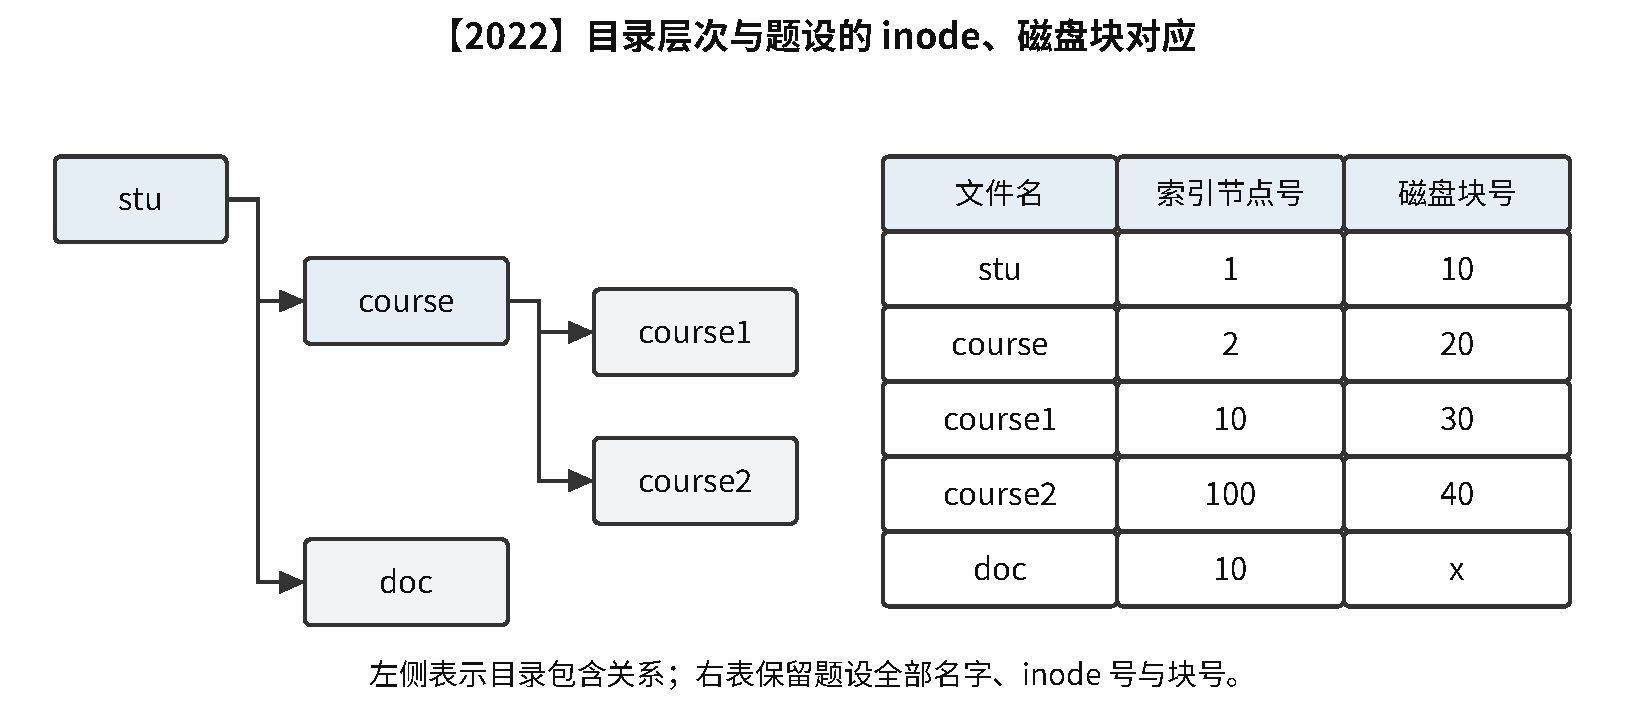
\includegraphics[width=0.96\textwidth,height=\textheight]{figures/OS_file_directory_2022.pdf}
\caption{stu、course 的目录层次，以及各文件的索引节点号和数据块号}\label{os-fig-directory2022}
\end{figure}

（1）目录文件 stu 中每个目录项的内容是什么？

（2）文件 doc 占用的磁盘块的块号 x 的值是多少？

（3）若目录文件 course 的内容已在内存，则打开文件 course1 并将其读入内存，需要读几个磁盘块？说明理由。

（4）若文件 course2 的大小增长到 6 MB，则为了存取 course2 需要使用该文件索引节点的哪几级间接地址项？说明理由。

\Needspace{6\baselineskip}

\textbf{解析。} （1）stu 的直接子项只有 course 和 doc。目录项存名字和 inode 号，不存其数据块号，故内容分别为 \texttt{(course,}\allowbreak{}\texttt{2)}、\texttt{(doc,}\allowbreak{}\texttt{10)}；course1、course2 的目录项在 course 中，不在 stu 中。图未列出 \texttt{.}、\texttt{..}，本问按图列出两个给定子项。

（2）doc 和 course1 的索引节点号同为 10，且属于同一文件系统，说明它们是同一个文件对象的两个名字。course1 的数据在 30 号磁盘块，因此 \(x=30\)。不是因为名字相似而共享，也不是把 inode 号 10 直接当作数据块号。

（3）按本问给出的缓存起点，course 的目录项可在内存查到，先取得 course1 的 inode 号 10。随后读入该 inode 所在的磁盘块，从 inode 得到数据块号 30，再读 30 号数据块，共 \textbf{2 个磁盘块}。打开所需的内存表项由系统建立，不另算作磁盘块；256 B 的 inode 放在磁盘块中，读取它仍按块计。题目只说目录内容已在内存，不能顺带认定文件 inode 和数据也已经缓存；若另给这些缓存命中条件，才相应减少次数。

（4）本题按 \(1\text{ MB}=1024\text{ KB}\) 计算，6 MB 文件需要

\[\frac{6\times1024\text{ KB}}{4\text{ KB}}=1536\text{ 个数据块}.\]

每个间接索引块容纳 \(4096/4=1024\) 个地址项。10 个直接项与一级间接项合计覆盖 \(10+1024=1034\) 个数据块，仍少 \(1536-1034=502\) 块；二级间接项可再覆盖 \(1024^2\) 个数据块。因此需用\textbf{一级和二级间接地址项}，不必用三级。这里的 1536 是用户数据块数，索引块另占空间；按先用直接区、再用各间接区的组织，一级区需要 1 个索引块，二级区需要 1 个二级索引块和其指向的 1 个一级索引块。

\subsection{例 6-8　先算地址覆盖，再比较 inode 与数据簇的上限}\label{os-ex6-8}

\noindent{}【2018】 某文件系统采用索引节点存放文件的属性和地址信息，簇大小为 4 KB。每个文件索引节点占 64 B，有 11 个地址项，其中直接地址项 8 个，一级、二级和三级间接地址项各 1 个，每个地址项长度为 4 B。请回答下列问题。

（1）该文件系统能支持的最大文件长度是多少？（给出计算表达式即可。）

（2）文件系统用 1M（\(1\mathrm{M}=2^{20}\)）个簇存放文件索引节点，用 512M 个簇存放文件数据。若一个图像文件的大小为 5600 B，则该文件系统最多能存放多少个这样的图像文件？

（3）若文件 F1 的大小为 6 KB，文件 F2 的大小为 40 KB，则该文件系统获取 F1 和 F2 最后一个簇的簇号需要的时间是否相同？为什么？

\Needspace{6\baselineskip}

\textbf{解析。} （1）一个索引簇可存 \(4096/4=1024\) 个簇号。直接、一级、二级、三级区分别覆盖 \(8\)、\(1024\)、\(1024^2\)、\(1024^3\) 个数据簇，所以最大文件长度为

\[L_{\max}=(8+1024+1024^2+1024^3)\times4096\text{ B}.\]

按二进制容量单位，这等于 4 TiB + 4 GiB + 4 MiB + 32 KiB。它只统计文件数据，不把索引簇自身算入用户文件长度。

（2）先独立计算两个容量限制。每个 inode 簇放 \(4096/64=64\) 个 inode，故 inode 区能容纳 \(2^{20}\times64=2^{26}=64\mathrm{M}\) 个文件。5600 B 大于一个簇而小于两个簇，每个图像占 \(\lceil5600/4096\rceil=2\) 个数据簇，数据区可容纳 \(512\mathrm{M}/2=256\mathrm{M}\) 个。两个数据簇都在 8 个直接地址项覆盖范围内，不额外占间接索引簇。因此最多存放

\[\min(64\mathrm{M},256\mathrm{M})=64\mathrm{M}=67\,108\,864\text{ 个图像文件}.\]

这里 M 表示个数的 \(2^{20}\) 倍；``还有数据簇''不能突破 inode 数量上限。计算采用题给的两个可用区域，不另假设目录占用或其他保留量。

（3）按本题比较的索引访问层级，时间不同。F1 占 \(\lceil6/4\rceil=2\) 个簇，末簇是逻辑簇 1，其簇号就在 inode 的直接项中。F2 占 \(40/4=10\) 个簇，末簇是逻辑簇 9；前 8 个逻辑簇 0---7 用直接项，逻辑簇 8---9 进入一级间接区，所以还须沿一级间接地址读索引簇，再取其第 1 项。

在 inode 同样已在内存、相关间接索引未缓存的共同起点下，F1 的末簇号可直接从内存取得，F2 多一次索引簇读盘。若连末簇数据也要读入，则路径分别是``数据簇''与``一级索引簇→数据簇''，为 1 次、2 次访盘。原问只求簇号，不能把目标数据簇的读取强行加进原问；若另有索引缓存命中，实际耗时还会改变。

\section{自测：沿名称与数据两条线检查}\label{os-6-review}

以下为原创回顾设问。

\begin{enumerate}
\def\labelenumi{\arabic{enumi}.}
\tightlist
\item
  关闭最后一个文件描述符，是否要求硬链接数减 1？
\item
  例6-3中，偏移恰好为 10240 B，属于直接区还是一级间接区？
\item
  某文件两个硬链接数从 2 减为 1，文件内容是否回收？软链接是否增加目标的硬链接计数？
\item
  管理 \(2^{20}\) 个块需要多少位图空间？若目前只有 1 个空闲块，位图是否只需 1 位？
\item
  同一 inode 能否由两个打开实例保存不同的当前偏移？
\end{enumerate}

\subsection{自测答案}\label{os-c06-h253}

\begin{enumerate}
\def\labelenumi{\arabic{enumi}.}
\tightlist
\item
  不要求。打开引用与硬链接计数分别描述运行中的打开和目录名字关系。
\item
  前 10 块覆盖偏移 0---10239，10240 是一级间接区第一个字节。
\item
  仍有一个硬链接，不回收内容。软链接只保存路径，不因此增加目标硬链接数。
\item
  \(2^{20}/8=2^{17}\) B，即 128 KB。位图仍为每个受管块保留一位。
\item
  可以，独立打开与 inode 共享是两个不同关系。
\end{enumerate}

\chapter{I/O 管理、设备软件与外存调度}\label{os-ch7}

应用说``读一个文件块''，设备却接收具体的命令、地址和长度。操作系统在中间完成命名、保护、排队、缓冲和状态通知。本章沿一个请求追踪软件与硬件的分工，再把缓冲时间和磁盘运动转成可计算的过程。

\section{设备、控制器、接口与端口}\label{os-7-1}

\textbf{设备}完成实际输入、输出或存储，\textbf{设备控制器}管理设备动作并向主机提供寄存器等接口。控制寄存器接收命令与参数，状态寄存器反映就绪、忙、错误等状态，数据寄存器或缓冲区承载数据。\textbf{端口}在此通常指可访问的接口寄存器位置，不是网络中传输层端口号。

独立编址的 I/O 端口由专门 I/O 指令访问；内存映射 I/O 把接口寄存器放入地址空间，通过相应访存指令访问，但访问副作用和缓存属性必须按设备规则处理。接口地址是控制器寄存器的地址，不是设备所保存文件的字节偏移。

\textbf{字符设备}通常按字符流组织，不适合按任意字节地址定位，例如终端；\textbf{块设备}按可寻址数据块组织，可进行块号访问，例如磁盘。网络设备按分组收发，还涉及通信地址和协议，不宜机械套成磁盘的寻道块模型。

独占设备在一次使用期间交给一个使用者；共享设备允许多个作业在一段时期内交替提交请求。共享不要求多个物理操作在同一瞬间执行。设备是否可寻址、是否共享、是否可随机访问是不同分类维度，不能把字符设备定义成``可按字节地址随机访问''。

\section{轮询、中断和 DMA：谁搬数据，谁等待}\label{os-7-2}

\textbf{程序查询或轮询}由 CPU 反复读状态，设备就绪时再执行数据传送。实现简单，但忙等期间 CPU 不能有效做别的工作。\textbf{中断方式}启动设备后允许 CPU 执行其他任务，设备在需要服务或完成时发中断，CPU 进入中断服务程序处理；若每次数据通过 CPU 的读写指令搬运，数据通路仍经过 CPU。

\textbf{DMA}由专门硬件按驱动设置的地址、长度和方向，在设备与内存之间传送数据。CPU 负责启动、异常和结束处理，不必逐字执行搬运指令；DMA 需要获得总线或内存访问机会，仍可能与 CPU 竞争存储带宽。DMA 结束通常通过中断通知，所以``DMA 与中断不能共存''不成立。

\begin{longtable}[]{@{}
  >{\raggedright\arraybackslash}p{(\columnwidth - 4\tabcolsep) * \real{0.2428}}
  >{\raggedright\arraybackslash}p{(\columnwidth - 4\tabcolsep) * \real{0.3543}}
  >{\raggedright\arraybackslash}p{(\columnwidth - 4\tabcolsep) * \real{0.4027}}@{}}
\toprule\noalign{}
\begin{minipage}[b]{\linewidth}\raggedright
控制方式
\end{minipage} & \begin{minipage}[b]{\linewidth}\raggedright
数据搬运的直接执行者
\end{minipage} & \begin{minipage}[b]{\linewidth}\raggedright
CPU 可以从什么工作中解脱
\end{minipage} \\
\midrule\noalign{}
\endhead
\bottomrule\noalign{}
\endlastfoot
轮询 & CPU 执行数据传送指令 & 通常不能免除状态忙等 \\
中断 & CPU 执行中断服务中的传送指令 & 不必连续轮询设备 \\
DMA & DMA 控制硬件 & 不必逐字/逐块执行软件搬运，但仍需初始化与完成处理 \\
\end{longtable}

请求 I/O 的线程是否阻塞，是接口语义问题；设备采用哪种传送控制，是硬件和驱动问题。一个阻塞读在中断或 DMA 工作期间可以睡眠；一个非阻塞请求也可立刻返回。不能从``DMA''一个词推出用户进程必处于阻塞态。

DMA 地址还要按系统规则提供：不能让设备任意写用户给出的地址。实际系统可能使用固定页、内核缓冲和 IOMMU 等机制；本书题目只要求按其给定的物理地址与控制模型推演，不把``DMA 无需 CPU 每字搬运''误写成``完全不需要操作系统参与''。

\section{I/O 软件层次与一次请求的完整路径}\label{os-7-3}

用户层 I/O 库组织格式和用户缓冲；系统调用进入内核。设备无关软件处理共同的命名、权限、缓冲、分配和错误接口；设备驱动程序把抽象请求变成控制器能执行的命令，设置寄存器并启动设备；中断处理在完成或异常通知后记录状态、推进请求并唤醒等待者。

\begin{figure}
\centering
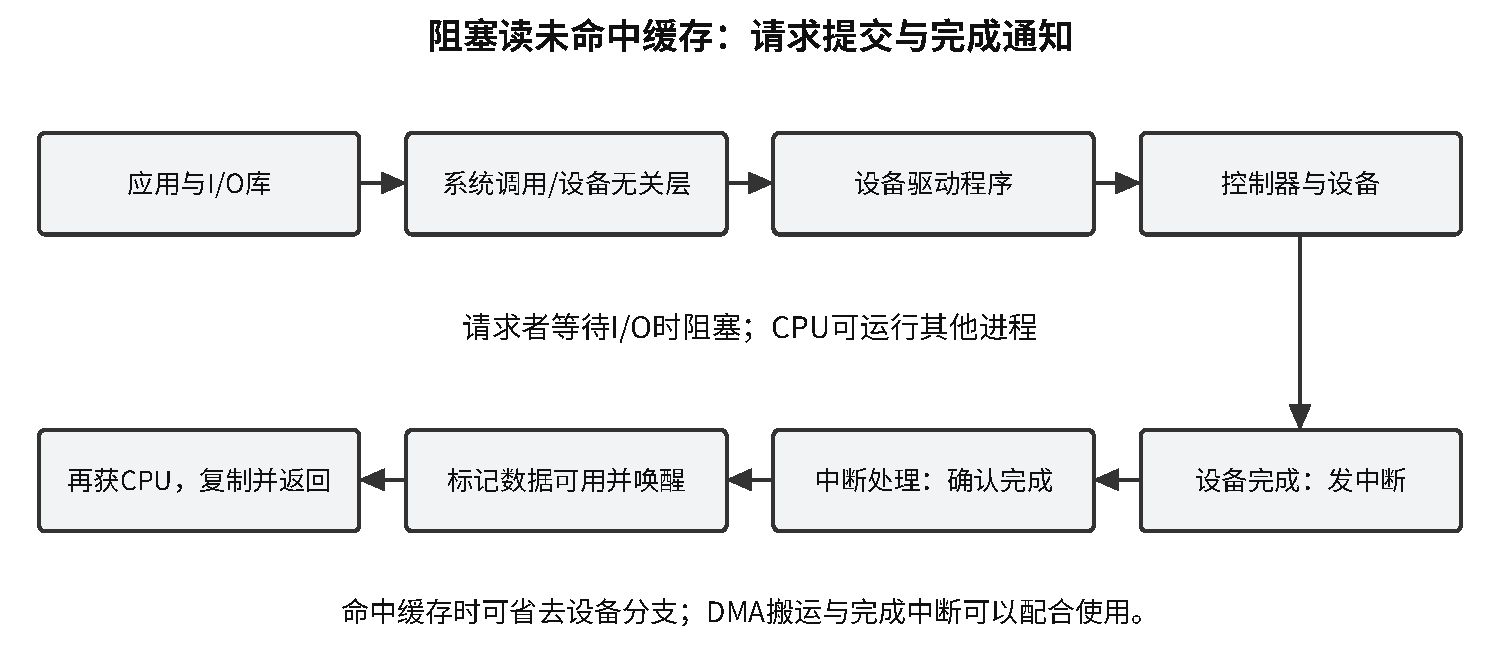
\includegraphics[width=0.95\textwidth,height=\textheight]{figures/OS_io_path.pdf}
\caption{提交路径向下，完成通知向上；唤醒以后仍由调度器决定何时运行}\label{os-fig-io}
\end{figure}

对一个缓存未命中的阻塞式磁盘读，连续过程可以是：应用发出 read，内核查找文件块并申请缓冲，驱动把请求排队、设置 DMA 并启动；调用者等待数据而阻塞，CPU 运行其他进程；设备完成后发中断，处理程序确认状态并标记缓冲可用，唤醒等待者；其再次运行时完成复制和返回。若数据早已缓存，设备分支可能整个省去。

\subsection{例 7-1　哪里需要知道具体设备参数}\label{os-ex7-1}

\noindent{}【2013】 用户程序发出磁盘 I/O 请求后，系统处理流程为：用户程序→系统调用处理程序→设备驱动程序→中断处理程序。其中，计算数据所在磁盘柱面号、磁头号和扇区号的程序是（　）。

A. 用户程序　　B. 系统调用处理程序　　C. 设备驱动程序　　D. 中断处理程序

\Needspace{6\baselineskip}

\textbf{解析。} 柱面、磁头和扇区是具体磁盘寻址参数，应由屏蔽设备差异的驱动处理，答案为 \textbf{C}。中断处理主要响应已发生的完成或异常事件，不是把每个初始请求都从文件逻辑位置重新规划一次。现代磁盘常接受逻辑块地址 LBA，内部几何转换可由设备完成；这不改变本题按传统 CHS 模型划分驱动职责的答案。

\section{阻塞、非阻塞与异步接口}\label{os-7-4}

\textbf{阻塞 I/O}在操作暂不能完成时，使调用线程等待；\textbf{非阻塞 I/O}在暂不能立即完成时返回相应状态，让程序决定重试、处理其他事务或等待通知。反复调用非阻塞接口也可能形成忙等，接口不阻塞不表示自动提高利用率。

\textbf{异步 I/O}把提交与完成分开，提交后程序继续执行，以后通过通知、完成队列等取得结果。非阻塞主要回答``本次调用等待不等待''，异步主要回答``操作完成如何与调用者联系''，不能把二者作为完全相同的术语。具体接口是否可能立即完成、如何报告部分完成，要按题设。

字符设备常有字符流、行缓冲等语义，块设备有块号和对齐约束，网络接口涉及发送、接收和连接/分组。设备无关性是给上层适当统一的抽象，不是强求所有设备具有完全一样的操作集合。

\section{缓冲：把输入、复制与计算放到同一时间线}\label{os-7-5}

缓冲在生产者和使用者之间暂存数据，可以缓和速度差、适配传送单位、允许阶段重叠。高速磁盘缓存还可利用重复访问、预读和延迟写，减少某些实际 I/O。缓冲区不改变设备本身的物理速度，也不会无条件消除所有等待。

设每块从设备输入系统缓冲耗时 \(T\)，从系统缓冲复制到用户工作区耗时 \(M\)，CPU 分析该块耗时 \(C\)。假定输入可与 CPU 工作重叠，复制与分析共用相应 CPU 资源不能互相重叠，只有一个用户工作区，并忽略其他开销。

\textbf{单缓冲}中，设备不能在缓冲尚未复制完时覆盖它；复制下一块也不能覆盖仍在分析的用户工作区。因此第一块先经 \(T+M\)，以后相邻复制完成点之间是 \(\max(T,C)+M\)，最后还要完成最后一块的分析。对 \(n\ge1\) 块：

\[T_{\mathrm{single}}=T+M+(n-1)[\max(T,C)+M]+C.\]

\textbf{双缓冲}允许设备填另一个系统缓冲，而 CPU 使用前一个。流水阶段可看成设备输入 \(T\) 与 CPU 的复制加分析 \(M+C\)，在上述资源模型下：

\[T_{\mathrm{double}}=T+(n-1)\max(T,M+C)+M+C.\]

这些是从阶段占用关系推出的公式。题目改成两个用户工作区、复制不用 CPU、半双工链路或其他限制时，先重画时间线，不能只凭``单缓冲/双缓冲''名称直接套式。

\subsection{例 7-2　首块要启动，末块要排空}\label{os-ex7-2}

\noindent{}【2011】 某文件占 10 个磁盘块，逐块读入主存缓冲，再送用户区分析。一个缓冲区与一个磁盘块大小相同，读一块到缓冲区为 100 μs，复制到用户区为 50 μs，CPU 分析一块为 50 μs。在单缓冲、双缓冲结构下，读入并分析完该文件的时间分别是（　）。

A. 1500 μs、1000 μs　　B. 1550 μs、1100 μs

C. 1550 μs、1550 μs　　D. 2000 μs、2000 μs

\begin{figure}
\centering
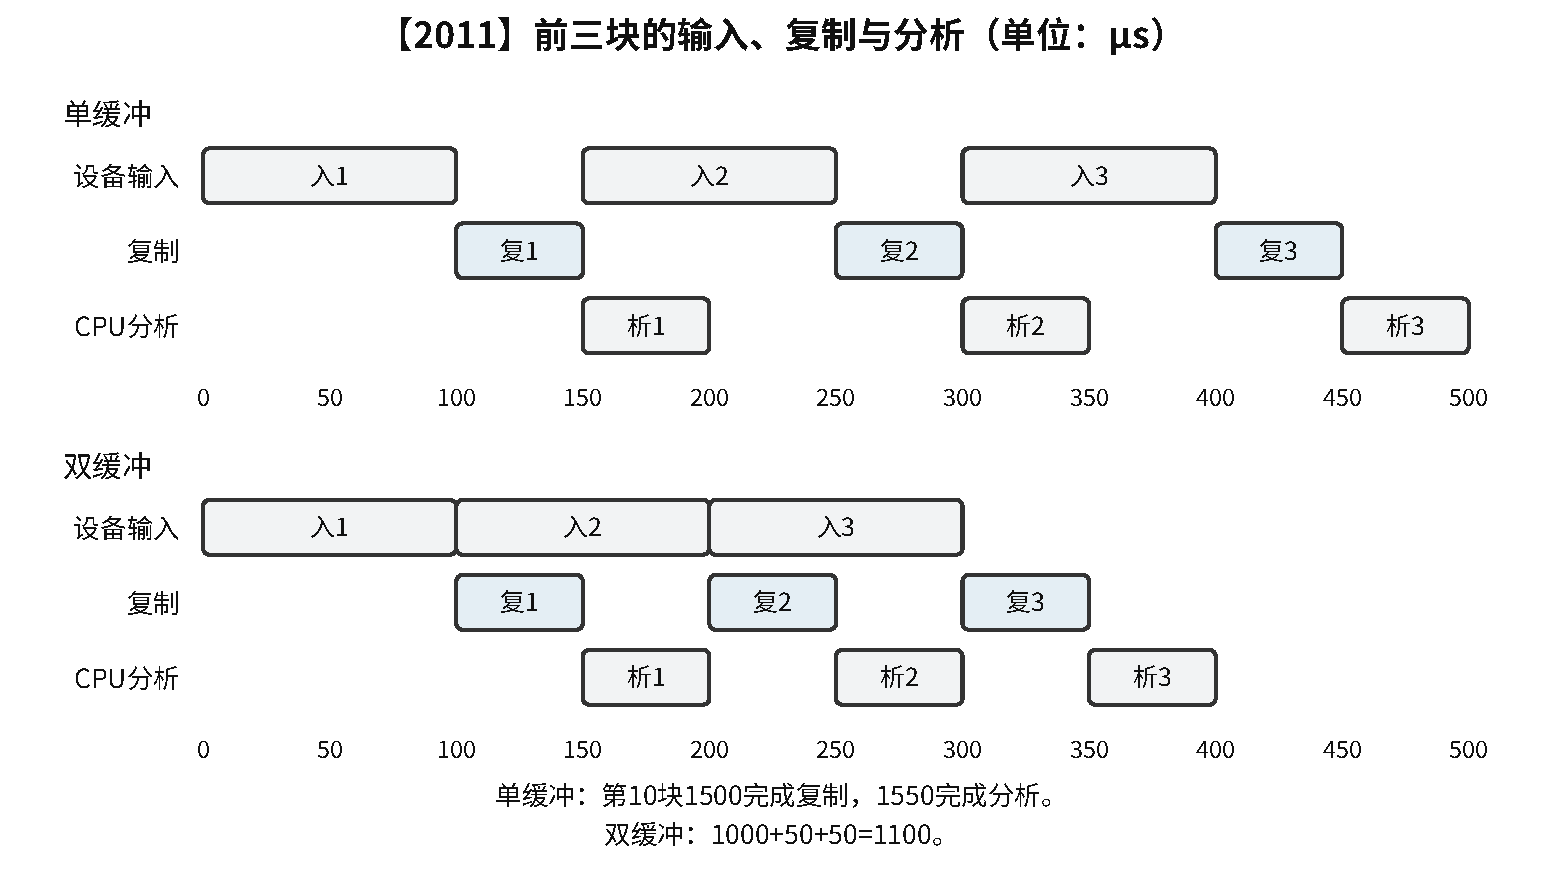
\includegraphics[width=0.96\textwidth,height=\textheight]{figures/OS_buffer_timeline.pdf}
\caption{前三块的时间线显示缓冲复用条件；第10块仍须完成复制和分析}\label{os-fig-buffertime}
\end{figure}

\Needspace{6\baselineskip}

\textbf{解析。} 单缓冲第 1 块输入 0---100，复制 100---150，分析 150---200；第 2 块可在第 1 块分析时开始输入，即 150---250，然后复制 250---300、分析 300---350。以后每 150 μs 推进一块，第 10 块复制结束为 1500 μs，再分析 50 μs，合计 1550 μs。

双缓冲第 1 块输入后，设备立即在另一缓冲输入第 2 块，即 100---200；CPU 同期完成第 1 块的复制和分析，也需 100 μs。10 块输入可连续到 1000 μs，最后一块再复制、分析各 50 μs，总计 1100 μs，答案为 \textbf{B}。只算稳定流水的块数而漏掉最后排空，会误得 A。

\subsection{循环缓冲与缓冲池}\label{os-c07-h85}

循环缓冲让若干缓冲区按环使用，分别维护下一可填和下一可取位置；必须区分空、已填满、正在使用等状态，不能在消费者读完之前覆盖。缓冲池把多个缓冲按空闲、输入、输出等用途组织，按请求分配与回收，可让多个活动复用。

缓冲管理既要选择大小、数量，也要协调生产与消费。双缓冲若输入远快于计算，设备仍会在两个缓冲都占用后等待；缓冲有限，不能让无限输入永远无阻塞。相关计数与互斥规则可回指第3章的有限缓冲区，数据传送与并发状态必须同时正确。

\section{设备分配、逻辑名称与驱动接口}\label{os-7-6}

设备分配要检查设备类型、访问权限、当前占用、逻辑名称到实际设备的映射，并选择可用设备与相关控制器、通道等资源。若需要的资源暂不可得，要按规则排队，不能只分配设备却忽略它必须使用的传输路径。资源逐项申请还可能与第4章的死锁条件相遇。

静态分配在作业开始前取得所需设备，减少运行中占有并等待，但利用率可能低；动态分配在使用时申请，更灵活，也需处理等待和安全。独占与共享是设备使用性质，静态与动态是分配时机，不能完全一一对应。

设备独立性让应用使用逻辑名称或统一接口，设备无关软件完成适当映射；更换设备通常调整映射和驱动，上层不必重写业务逻辑。驱动还须遵守操作系统的入口、同步、内存和完成通知接口；同一硬件的驱动不能因此无修改地用于所有操作系统。

设备释放后，要更新控制结构、处理队列并通知合适等待者。内核记录``空闲''以前必须确认上一请求确实结束，避免两个使用者同时认为自己拥有设备。

\section{SPOOLing：先进入磁盘井，再使用独占设备}\label{os-7-7}

\textbf{SPOOLing}利用磁盘上的输入井、输出井和相应进程，把低速独占设备的使用与应用运行分开，形成假脱机工作方式。输入进程把设备数据预先送入输入井，作业随后从井取数据；输出请求先进入输出井，由输出进程按队列统一送到真实设备，井管理负责记录请求与存储位置等。

打印时，多个进程可以分别提交打印文件和请求，提交后继续做别的工作；打印守护进程再逐份占用物理打印机。用户看到逻辑上可共享的打印服务，打印机仍一次打印一个任务。不能把``将独占设备改造成共享设备''理解成硬件突然能同时输出多份互不干扰的纸张。

井通常在磁盘，不是简单把所有输出永久留在内存；SPOOLing 也不是用一台专用外围机完全脱离主机运行。多道程序设计让井管理、设备服务与用户作业可以并发，缓冲协调暂存数据，二者分别承担不同作用。

\section{磁盘结构、地址与格式化}\label{os-7-8}

磁盘盘面有磁道，同半径磁道形成柱面，磁道再分扇区。移动磁头到目标磁道需要\textbf{寻道时间}，等待目标扇区转到磁头下需要\textbf{旋转延迟}，实际数据经过磁头需要\textbf{传输时间}。常规平均模型为

\[T_{\mathrm{access}}=T_{\mathrm{seek}}+T_{\mathrm{rotation}}+T_{\mathrm{transfer}}.\]

若转速为 \(r\) 转/秒，一圈为 \(1/r\) 秒，随机角位置下平均旋转延迟为 \(1/(2r)\)。若题目直接给 \(r\) 秒/转，则平均延迟为 \(r/2\)，两种 r 单位不能混用。一个磁道能传 N B，连续读取 b B、忽略跨道与间隙时，传输时间近似为 \((b/N)/r\) 秒。

例如 7200 转/分为 120 转/秒，一圈约 8.333 ms，平均旋转延迟约 4.167 ms。若平均寻道 5 ms、目标连续数据传输 0.5 ms，则平均访问约 9.667 ms。这是\textbf{原创单位示例}，用于把 rpm 换成时间；跨道访问若需额外寻道，不能继续当作同一连续磁道传输。

\subsection{例 7-3　柱面、盘面、扇区是混合进位}\label{os-ex7-3}

\noindent{}〖5.3-016〗 磁盘有 100 个柱面，每柱面 8 个磁道，每磁道 8 个扇区。文件 A 有 6400 个逻辑记录，每记录与扇区大小相同，顺序存放；第 0 个记录在 (0 号柱面、0 号盘面、0 号扇区)。磁盘地址 (78、6、6) 存放文件的第几个逻辑记录？

A. 5045　　B. 5046　　C. 5047　　D. 5048

\Needspace{6\baselineskip}

\textbf{解析。} 先跨 78 个柱面，每柱面 \(8\times8=64\) 个记录，再跨本柱面的 6 个盘面，最后跨 6 个扇区，得到 \(78\times64+6\times8+6=5046\)，答案为 \textbf{B}。题目明确从 0 编号，不能再加 1。反算时先除 64 取柱面，余数再除 8 取盘面，最后余数为扇区。

\subsection{分区、物理格式化和逻辑格式化}\label{os-c07-h127}

物理格式化或低级格式化建立控制器识别的扇区结构及校验等信息；分区划分可独立使用的逻辑区域；逻辑格式化在某区域上建立文件系统结构，如超级块、根目录和空闲管理结构。创建文件系统不是每次开机都要做的初始化。

\subsection{例 7-4　根目录属于文件系统，不属于扇区编码}\label{os-ex7-4}

\noindent{}【2017】 下列选项中，磁盘逻辑格式化程序所做的工作是（　）。

Ⅰ. 对磁盘进行分区　　Ⅱ. 建立文件系统根目录

Ⅲ. 确定磁盘扇区校验码所占位数　　Ⅳ. 初始化保存空闲磁盘块信息的数据结构

A. 仅Ⅱ　　B. 仅Ⅱ、Ⅳ　　C. 仅Ⅲ、Ⅳ　　D. 仅Ⅰ、Ⅱ、Ⅳ

\Needspace{6\baselineskip}

\textbf{解析。} Ⅱ、Ⅳ创建的是文件系统结构；Ⅰ是分区，Ⅲ属于物理扇区组织。答案为 \textbf{B}。传统主引导扇区、分区引导区域和文件系统数据区的建立时机也不同，不能见到``引导''就一律归到 BIOS 或逻辑格式化。

\section{磁盘调度：把运动顺序和运动距离分开}\label{os-7-9}

\textbf{FCFS}按请求到达次序服务，公平直观，但相邻请求可能使磁头来回移动。\textbf{SSTF}每次选离当前磁头最近的请求，可减少当前一步的寻道，但不是求整个序列的全局最短路径；远处请求可能长期被新来的近处请求越过。

\textbf{SCAN}沿一个方向服务，达到规定端点后反向；\textbf{LOOK}到该方向最后一个请求便反向，不必到物理端点。\textbf{C-SCAN}只在一个方向服务，到端点后回到另一端，返回过程中不服务；\textbf{C-LOOK}在本方向最后请求处回跳到另一侧第一个请求。回跳会不会计入移动距离、是否规定到物理端点、何时停止统计，要按题干，不能只看算法名。

下表按物理端点与最后请求位置区分扫描算法。若题干另给折返、回跳或停止规则，应按具体规则重建轨迹。

\begin{longtable}[]{@{}
  >{\raggedright\arraybackslash}p{(\columnwidth - 8\tabcolsep) * \real{0.1647}}
  >{\raggedright\arraybackslash}p{(\columnwidth - 8\tabcolsep) * \real{0.2057}}
  >{\raggedright\arraybackslash}p{(\columnwidth - 8\tabcolsep) * \real{0.2076}}
  >{\raggedright\arraybackslash}p{(\columnwidth - 8\tabcolsep) * \real{0.1941}}
  >{\raggedright\arraybackslash}p{(\columnwidth - 8\tabcolsep) * \real{0.2276}}@{}}
\toprule\noalign{}
\begin{minipage}[b]{\linewidth}\raggedright
算法
\end{minipage} & \begin{minipage}[b]{\linewidth}\raggedright
怎样选择、沿什么方向服务
\end{minipage} & \begin{minipage}[b]{\linewidth}\raggedright
折返或回跳的位置
\end{minipage} & \begin{minipage}[b]{\linewidth}\raggedright
返回途中是否服务
\end{minipage} & \begin{minipage}[b]{\linewidth}\raggedright
等待方面的边界
\end{minipage} \\
\midrule\noalign{}
\endhead
\bottomrule\noalign{}
\endlastfoot
FCFS & 按请求到达顺序，方向可来回改变 & 无固定端点要求 & 不设专门回跳阶段 & 后到者不插队；前面的请求仍可能造成很长等待 \\
SSTF & 每次选距当前磁头最近的请求 & 无固定端点要求 & 不设专门回跳阶段 & 持续近处新请求可能越过远处请求，存在饥饿风险 \\
SCAN & 沿当前方向逐个服务，随后反向服务 & 到规定的物理端点再反向 & 反向扫描仍服务 & 扫描持续推进时按方向轮到；不同位置的服务间隔可不同 \\
LOOK & 同 SCAN，沿两个方向服务 & 本方向已无待处理请求便反向 & 反向扫描仍服务 & 省去无请求的端段；等待仍受负载和扫描推进规则约束 \\
C-SCAN & 只沿规定的一个方向服务 & 到物理端点，再回到另一物理端点 & 回跳不服务 & 循环服务次序使位置机会较均匀；不直接给出固定时间上界 \\
C-LOOK & 只沿规定的一个方向服务 & 本方向最后请求处，回到另一侧首个待处理请求 & 回跳不服务，到目标后恢复服务 & 缩短无请求的端段；循环次序仍需配合有限处理时间等条件 \\
\end{longtable}

对固定有限的一批请求，且每个请求处理时间有限时，SSTF 也会处理完，不能把``可能饥饿''说成``必然饥饿''。持续到达时，扫描能否保持前进还与新请求的接纳和服务规则有关；没有请求耗时、负载及推进条件，就不能宣称任何扫描变体具有无条件的固定等待上界。回跳不服务也不等于物理移动耗时为零。

\subsection{例 7-5　方向决定先服务哪一侧}\label{os-ex7-5}

\noindent{}【2015】 某硬盘有 200 个磁道，最外侧磁道号为 0，请求序列为 130、42、180、15、199。当前磁头位于 58 号磁道，从外侧向内侧移动。按 SCAN 处理完这些请求，磁头移动的磁道数为（　）。

A. 208　　B. 287　　C. 325　　D. 382

\begin{figure}
\centering
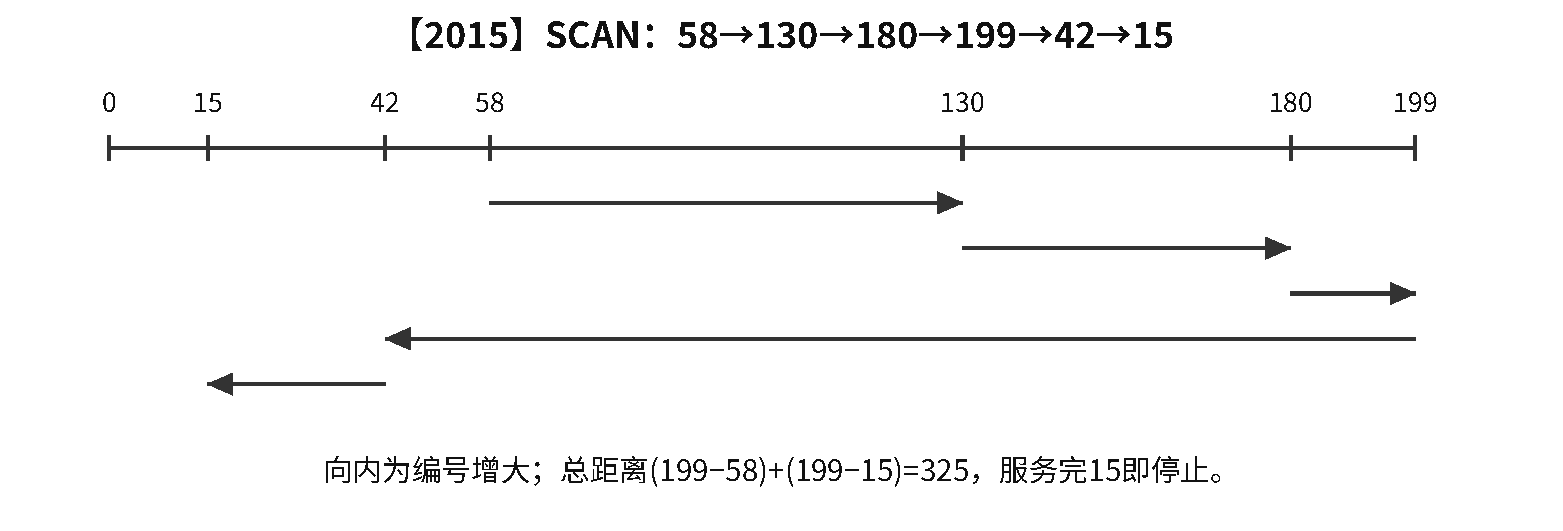
\includegraphics[width=0.96\textwidth,height=\textheight]{figures/OS_scan.pdf}
\caption{先向编号增加方向，再反向；本题最高请求恰为物理端点199}\label{os-fig-scan}
\end{figure}

\Needspace{6\baselineskip}

\textbf{解析。} 向内是编号增大，先服务 130、180、199，再反向服务 42、15。移动距离为 \((199-58)+(199-15)=141+184=325\)，答案为 \textbf{C}。不能按原输入序列依次访问，那是 FCFS；也不能先服务距 58 最近的 42，那是 SSTF 的首步。

本题最高请求就是端点 199，因此 SCAN 与 LOOK 恰好有相同折返点，不能凭这道题认为两算法永远相同。处理完最后请求 15 就停止统计，也不应继续加到 0 的距离。

若仅用相同数据比较算法：FCFS 按给定序列移动共 \(72+88+138+165+184=647\)；SSTF 依次 42、15、130、180、199，移动 \(16+27+115+50+19=227\)。这是题后方法比较，原题仍只问 SCAN；不同方法应各自重建顺序，不能复用另一个算法的轨迹。

调度主要影响寻道，但布局、顺序读预取等也能改变旋转和传输开销。把``磁头移动更少''直接当作``任何情况下总 I/O 时间最短''，忽略了请求大小、缓存、旋转位置及设备内部重排等条件。

\section{SSD：没有寻道，不等于没有管理开销}\label{os-7-10}

SSD 采用闪存，访问不需要机械寻道与旋转。闪存通常按页读取或编程，按更大的擦除块擦除；已写内容一般不能像内存字节那样任意原地覆盖，修改常通过异地写入并更新映射实现。\textbf{闪存转换层 FTL}维护逻辑地址到实际闪存位置的映射，与文件系统的文件偏移映射不是同一层。

异地更新使旧页失效，垃圾回收选择块，把仍有效内容迁走，再擦除整块以供后续使用。这会增加内部写入量，形成写放大；备用空间和回收策略会影响性能，不能只用接口带宽计算每次小写的真实代价。

擦写次数有限，\textbf{磨损均衡}避免少量块被反复使用。动态磨损均衡主要在新写入时平衡可选空闲块；静态磨损均衡还迁移长期不变的冷数据，让长期占用低磨损块的空间也参与使用。目的是均衡磨损、延长寿命，不保证每次请求更快。

TRIM 等通知让设备知道哪些逻辑数据已不再需要，有助于回收；文件删除、文件系统取消映射和设备实际擦除也不是同一瞬间。由于没有机械位置，传统寻道调度的优势不再原样成立，但请求合并、公平性、队列深度与写入管理仍有意义。

\section{综合例题：从等待事件到设备地址}\label{os-7-11}

\subsection{例 7-6　一次键盘输入怎样使阻塞者重新获得运行资格}\label{os-ex7-6}

\noindent{}【2023】 进程 P 通过执行系统调用从键盘接收一个字符的输入，已知此过程中与进程 P 相关的操作包括：①将进程 P 插入就绪队列；②将进程 P 插入阻塞队列；③将字符从键盘控制器读入系统缓冲区；④启动键盘中断处理程序；⑤进程 P 从系统调用返回；⑥用户在键盘上输入一个字符。以上编号①---⑥仅用于标记操作，与操作的先后顺序无关。请回答下列问题。

（1）按照正确的操作顺序，操作①的前一个和后一个操作分别是上述操作中的哪一个？操作⑥的后一个操作是上述操作中的哪一个？

（2）在上述哪个操作之后 CPU 一定从进程 P 切换到其他进程？在上述哪个操作之后 CPU 调度程序才能选中进程 P 执行？

（3）完成上述哪个操作的代码属于键盘驱动程序？

（4）键盘中断处理程序执行时，进程 P 处于什么状态？CPU 处于内核态还是用户态？

\Needspace{6\baselineskip}

\textbf{解析。} 先把六个操作放入一次完整请求中。P 执行系统调用，经受控入口进入内核；此时字符尚未输入，P 等待该事件，执行②进入阻塞队列，让出 CPU。用户随后执行⑥，键盘控制器产生中断请求；CPU 响应后转入内核入口，执行④启动键盘中断处理。处理代码执行③，把控制器中的字符读到系统缓冲区；数据可用后执行①，唤醒 P。P 以后被调度运行，继续尚未完成的系统调用，按调用语义把结果交给用户，最后执行⑤返回。

因此，在题目列出的六个操作之间，先后顺序是

\textbf{② → ⑥ → ④ → ③ → ① → ⑤。}

（1）①的前一个操作是 \textbf{③}，后一个操作是 \textbf{⑤}；⑥的后一个操作是 \textbf{④}。这里``前一个、后一个''只比较题列操作，①与⑤之间仍可有中断返回、等待调度、恢复执行等步骤，不能理解为相邻的两条机器指令。

（2）\textbf{②之后}，P 已阻塞，不能继续作为当前运行者，CPU 转去运行其他进程；若没有其他普通就绪进程，则进入系统的空闲执行路径。\textbf{①之后}，P 才恢复可调度资格。就绪不等于已经运行，更不保证中断处理一结束就必然选中 P。

（3）完成 \textbf{③} 的代码属于键盘驱动程序：它知道控制器接口，执行具体的 I/O 读操作并把字符放入系统缓冲。硬件产生中断请求、CPU 响应中断和驱动代码读字符是不同步骤。这里的字符搬运由执行驱动代码的 CPU 完成，不能因第7章讲过 DMA 就改写成 DMA 自动搬运。

（4）在键盘中断处理入口及读取字符的阶段，P 仍在阻塞队列中，处于\textbf{阻塞态}；处理数据后执行①才转为就绪。CPU 执行内核的中断处理代码，处于\textbf{内核态}。被中断的当前执行者可能是其他进程，内核正在为 P 完成 I/O 并不意味着 P 此刻就在 CPU 上运行。硬件响应负责受控转入并保存体系结构规定的必要状态，入口和驱动代码再保存其余现场、取数据并更新进程状态。

\subsection{例 7-7　把簇号转换成柱面，再逐步执行 SSTF}\label{os-ex7-7}

\noindent{}【2019】 某计算机系统中的磁盘有 300 个柱面，每个柱面有 10 个磁道，每个磁道有 200 个扇区，扇区大小为 512 B。文件系统的每个簇包含 2 个扇区。请回答下列问题。

（1）磁盘的容量是多少？

（2）假设磁头在 85 号柱面上，此时有 4 个磁盘访问请求，簇号分别为 100260、60005、101660 和 110560。若采用最短寻道时间优先（SSTF）调度算法，则系统访问簇的先后次序是什么？

（3）第 100530 簇在磁盘上的物理地址是什么？将簇号转换成磁盘物理地址的过程由 I/O 系统的什么程序完成？

\Needspace{6\baselineskip}

\textbf{解析。} （1）先按物理扇区计总容量，簇只是文件系统的分配单位，不会把物理容量再乘 2。

\[C=300\times10\times200\times512=307\,200\,000\text{ B}=300\,000\text{ KB}.\]

本式按 \(1\text{ KB}=1024\text{ B}\)。每簇 \(2\times512=1024\) B，每柱面有 \(10\times200/2=1000\) 个簇，所以也可用 \(300\times1000\times1024\) B 复核。

（2）本题按从 0 开始的线性簇号，把簇号除以 1000 取整得到柱面号。四个请求的柱面依次为 100、60、101、110。SSTF 每完成一次访问，就以新的柱面重新比较剩余请求，不能只按距初始柱面 85 的距离排序。

\begin{longtable}[]{@{}
  >{\raggedright\arraybackslash}p{(\columnwidth - 6\tabcolsep) * \real{0.2196}}
  >{\raggedright\arraybackslash}p{(\columnwidth - 6\tabcolsep) * \real{0.3257}}
  >{\raggedright\arraybackslash}p{(\columnwidth - 6\tabcolsep) * \real{0.2349}}
  >{\raggedright\arraybackslash}p{(\columnwidth - 6\tabcolsep) * \real{0.2196}}@{}}
\toprule\noalign{}
\begin{minipage}[b]{\linewidth}\raggedright
当前柱面
\end{minipage} & \begin{minipage}[b]{\linewidth}\raggedright
剩余请求的柱面与距离
\end{minipage} & \begin{minipage}[b]{\linewidth}\raggedright
选中的簇
\end{minipage} & \begin{minipage}[b]{\linewidth}\raggedright
到达柱面
\end{minipage} \\
\midrule\noalign{}
\endhead
\bottomrule\noalign{}
\endlastfoot
85 & 100：15；60：25；101：16；110：25 & 100260 & 100 \\
100 & 60：40；101：1；110：10 & 101660 & 101 \\
101 & 60：41；110：9 & 110560 & 110 \\
110 & 60：50 & 60005 & 60 \\
\end{longtable}

因此访问顺序为 \textbf{100260、101660、110560、60005}。总柱面移动量可复核为 \(15+1+9+50=75\)；原问只要求顺序，不需假设转速或旋转位置。

（3）每磁道 \(200/2=100\) 个簇。先分出柱面，再分出柱面内磁道及磁道内簇位置：

\[100530=100\times1000+530,\qquad530=5\times100+30.\]

故柱面号为 100，磁头（盘面）号为 5。磁道内第 30 簇由第 \(30\times2=60\) 和 61 号扇区组成，所以该簇的起始物理地址为 \textbf{（100 号柱面，5 号磁头，60 号扇区）}，随后还有同一磁道的 61 号扇区。这里各字段都按本题的 0 基编号模型，不能额外加 1。

簇号到该传统物理地址的转换由\textbf{磁盘驱动程序}完成：上层给出抽象访问位置，驱动按设备参数形成具体命令；中断处理在设备通知完成时确认状态，不能代替发起请求前的地址转换。若实际设备以 LBA 接口隐藏几何布局，转换分工可不同，本题按给定 CHS 模型回答。

\section{自测：先找可重叠阶段，再核单位}\label{os-7-review}

以下为原创回顾设问。

\begin{enumerate}
\def\labelenumi{\arabic{enumi}.}
\tightlist
\item
  DMA 期间 CPU 能运行其他进程，是否意味着传输完全不与 CPU 竞争资源？
\item
  例7-2若只有 1 块数据，单、双缓冲各需多久？
\item
  改用 LOOK 后，例7-5总移动为何不变？若最高请求不是 199，会影响哪里？
\item
  6000 转/分的磁盘，随机角位置下平均旋转延迟是多少？
\item
  SSD 删除一页数据后，能否立即按这一页为单位完成擦除？
\end{enumerate}

\subsection{自测答案}\label{os-c07-h261}

\begin{enumerate}
\def\labelenumi{\arabic{enumi}.}
\tightlist
\item
  不能。DMA 与 CPU 可能竞争总线、内存带宽等，且还要 CPU 完成启动和结束处理。
\item
  都需 \(100+50+50=200\) μs。一个块没有后续输入可以重叠，双缓冲不会自动减半时间。
\item
  本题最后的向内请求正好为物理端点。若最高请求更小，LOOK 提前折返，SCAN 仍按端点规则移动。
\item
  100 转/秒，一圈 10 ms，平均半圈为 5 ms。
\item
  通常不能。编程与读取以页为单位，擦除以较大的擦除块为单位，要结合有效页迁移和垃圾回收。
\end{enumerate}
